\documentclass{beamer}

\usepackage{multimedia}

\usetheme{metropolis}

\title{Punch Out Model Synthesis}
\subtitle{A Stochastic Algorithm for Constraint Based Tiling Generation}
\date{November 19th, 2024}
\author{Zzyv Zzyzek}
\begin{document}

\newcommand{\specialcell}[2][c]{\begin{tabular}[#1]{@{}l@{}}#2\end{tabular}}
\newcommand{\specialcellCenter}[2][c]{\begin{tabular}[#1]{@{}c@{}}#2\end{tabular}}

  \maketitle

  %\begin{frame}{Table of contents}
  %  \setbeamertemplate{section in toc}[sections numbered]
  %  \tableofcontents[hideallsubsections]
  %\end{frame}

  %\section{Introduction}

  \begin{frame}[fragile]{Introduction}
    \textbf{Punch Out Model Synthesis} (\textit{POMS})
    A Constraint Based Tiling Generation (\textit{CBTG}) algorithm:
    \begin{itemize}
      \item Works on large grids
      \item Minimal setup requirements
      \item Resiliance to contradiction
    \end{itemize}
  \end{frame}

  \begin{frame}[fragile]{Introduction}
    %Constraint Based Tiling Generation (\textit{CBTG})
    \begin{columns}[T,onlytextwidth]
      \column{0.5\textwidth}
        \begin{block}{Definitions}
          \begin{itemize}
            \item \textit{Grid} composed of \textit{cells}
            \item Each \textit{cell} can hold $D$ \textit{tiles}
            \item Pairwise tile \textit{constraints} in each dimension ($\pm X, \pm Y, \pm Z$)
          \end{itemize}
        \end{block}
      \column{0.5\textwidth}
        \begin{block}{Example}
          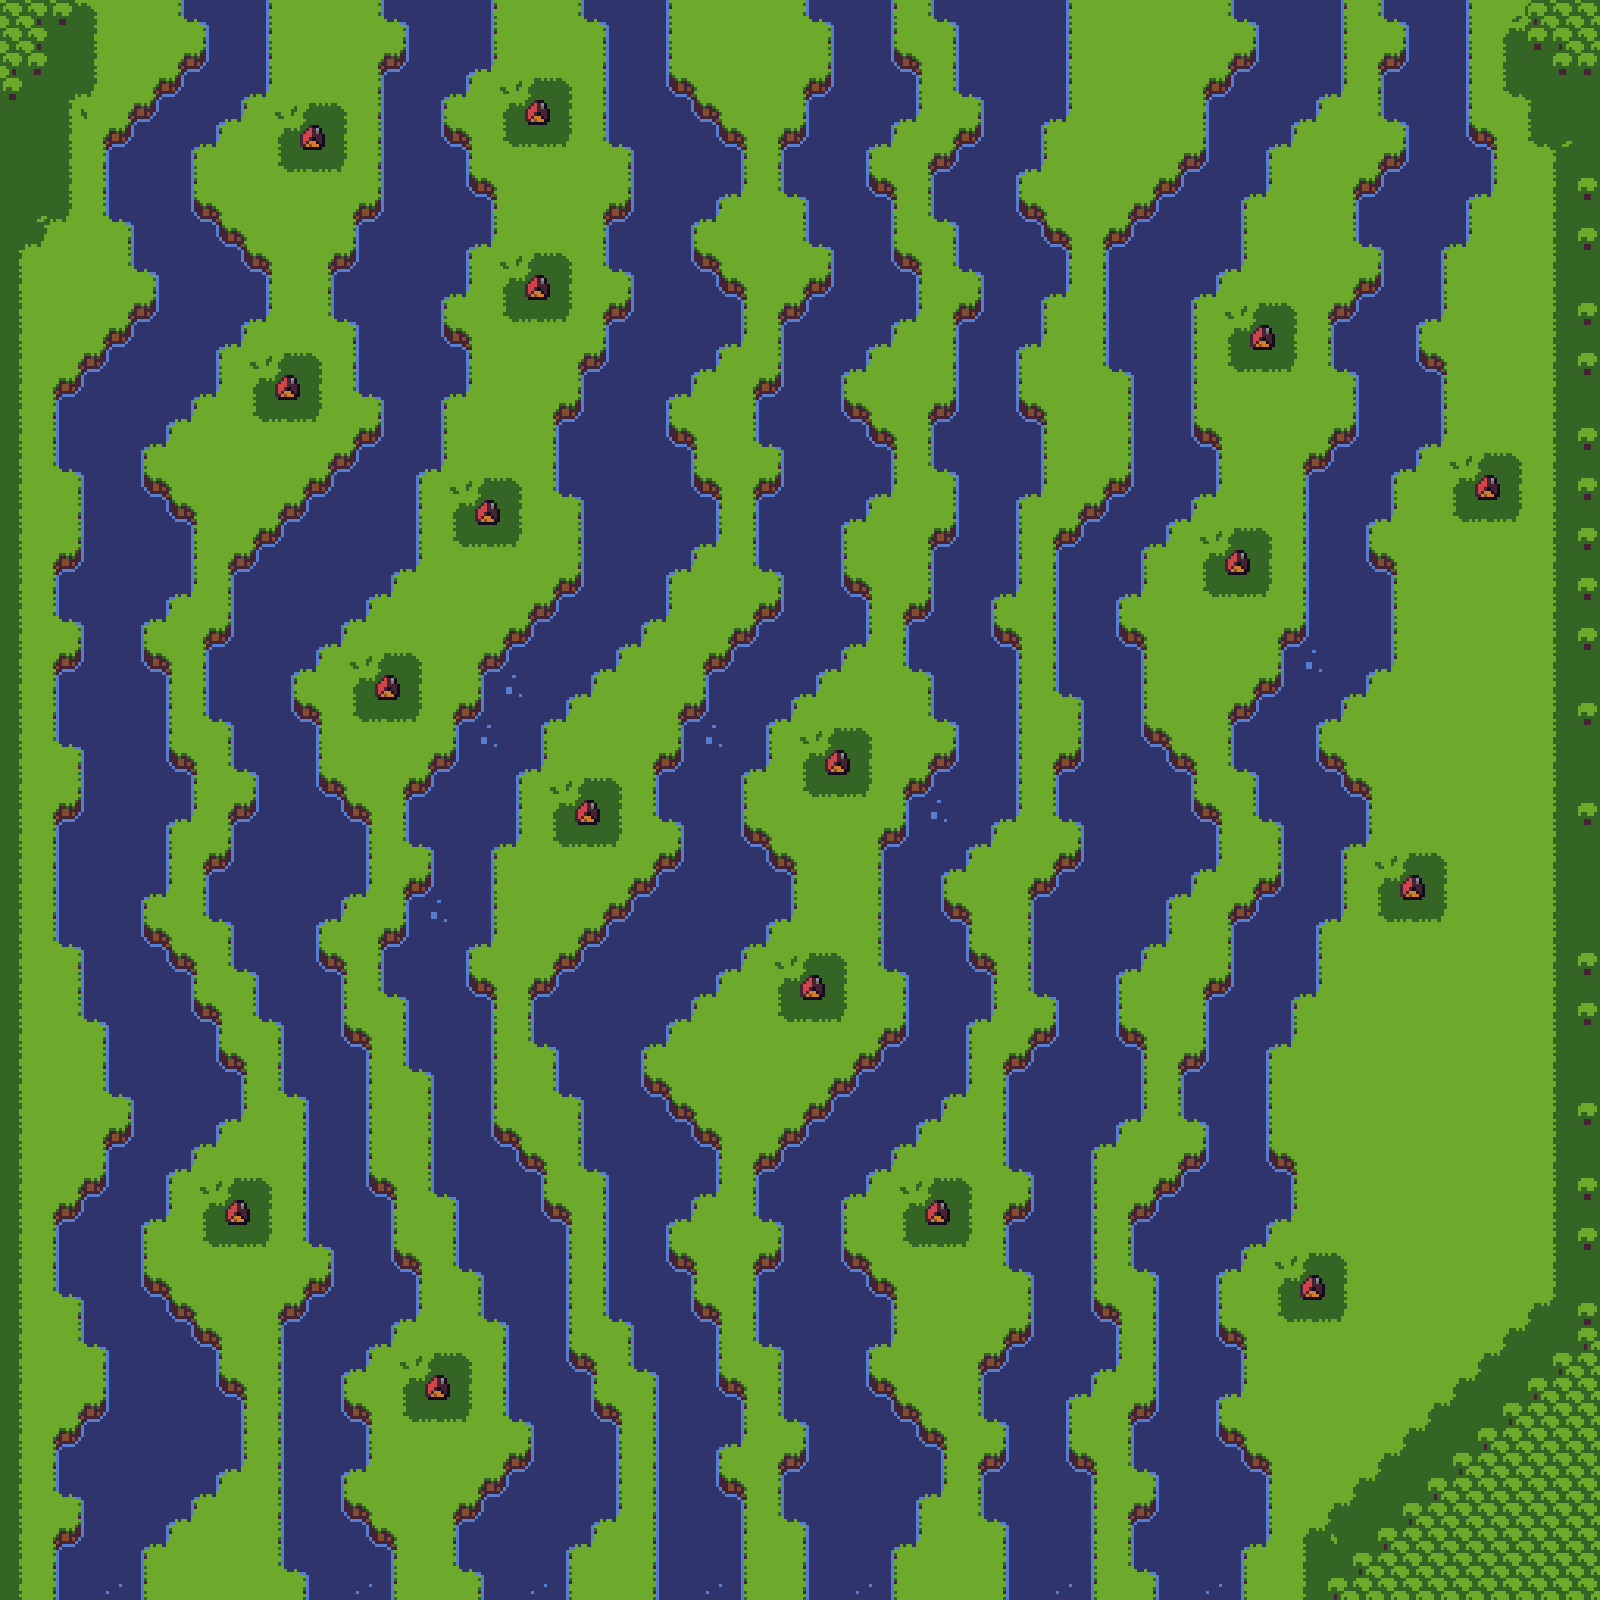
\includegraphics[width=0.9\textwidth]{img/forestmicro_64x64.pdf}
        \end{block}
    \end{columns}
  \end{frame}


%  \begin{frame}[fragile]{Introduction}
%    Constraint Based Tiling Generation (\textit{CBTG})
%    \begin{columns}[T,onlytextwidth]
%      \column{0.5\textwidth}
%        \begin{block}{Definitions}
%
%          \hfill \\
%          A \textit{realization} is a \textit{grid} that \\
%          has a single \textit{tile} at each \\
%          \textit{cell} respecting the \textit{constraints}.
%          \hfill \\
%          \hfill \\
%          If a cell has no tiles left, no \\
%          realization is possible and is
%          considered a \textit{contradiction}.
%        \end{block}
%      \column{0.5\textwidth}
%        \begin{block}{Example}
%          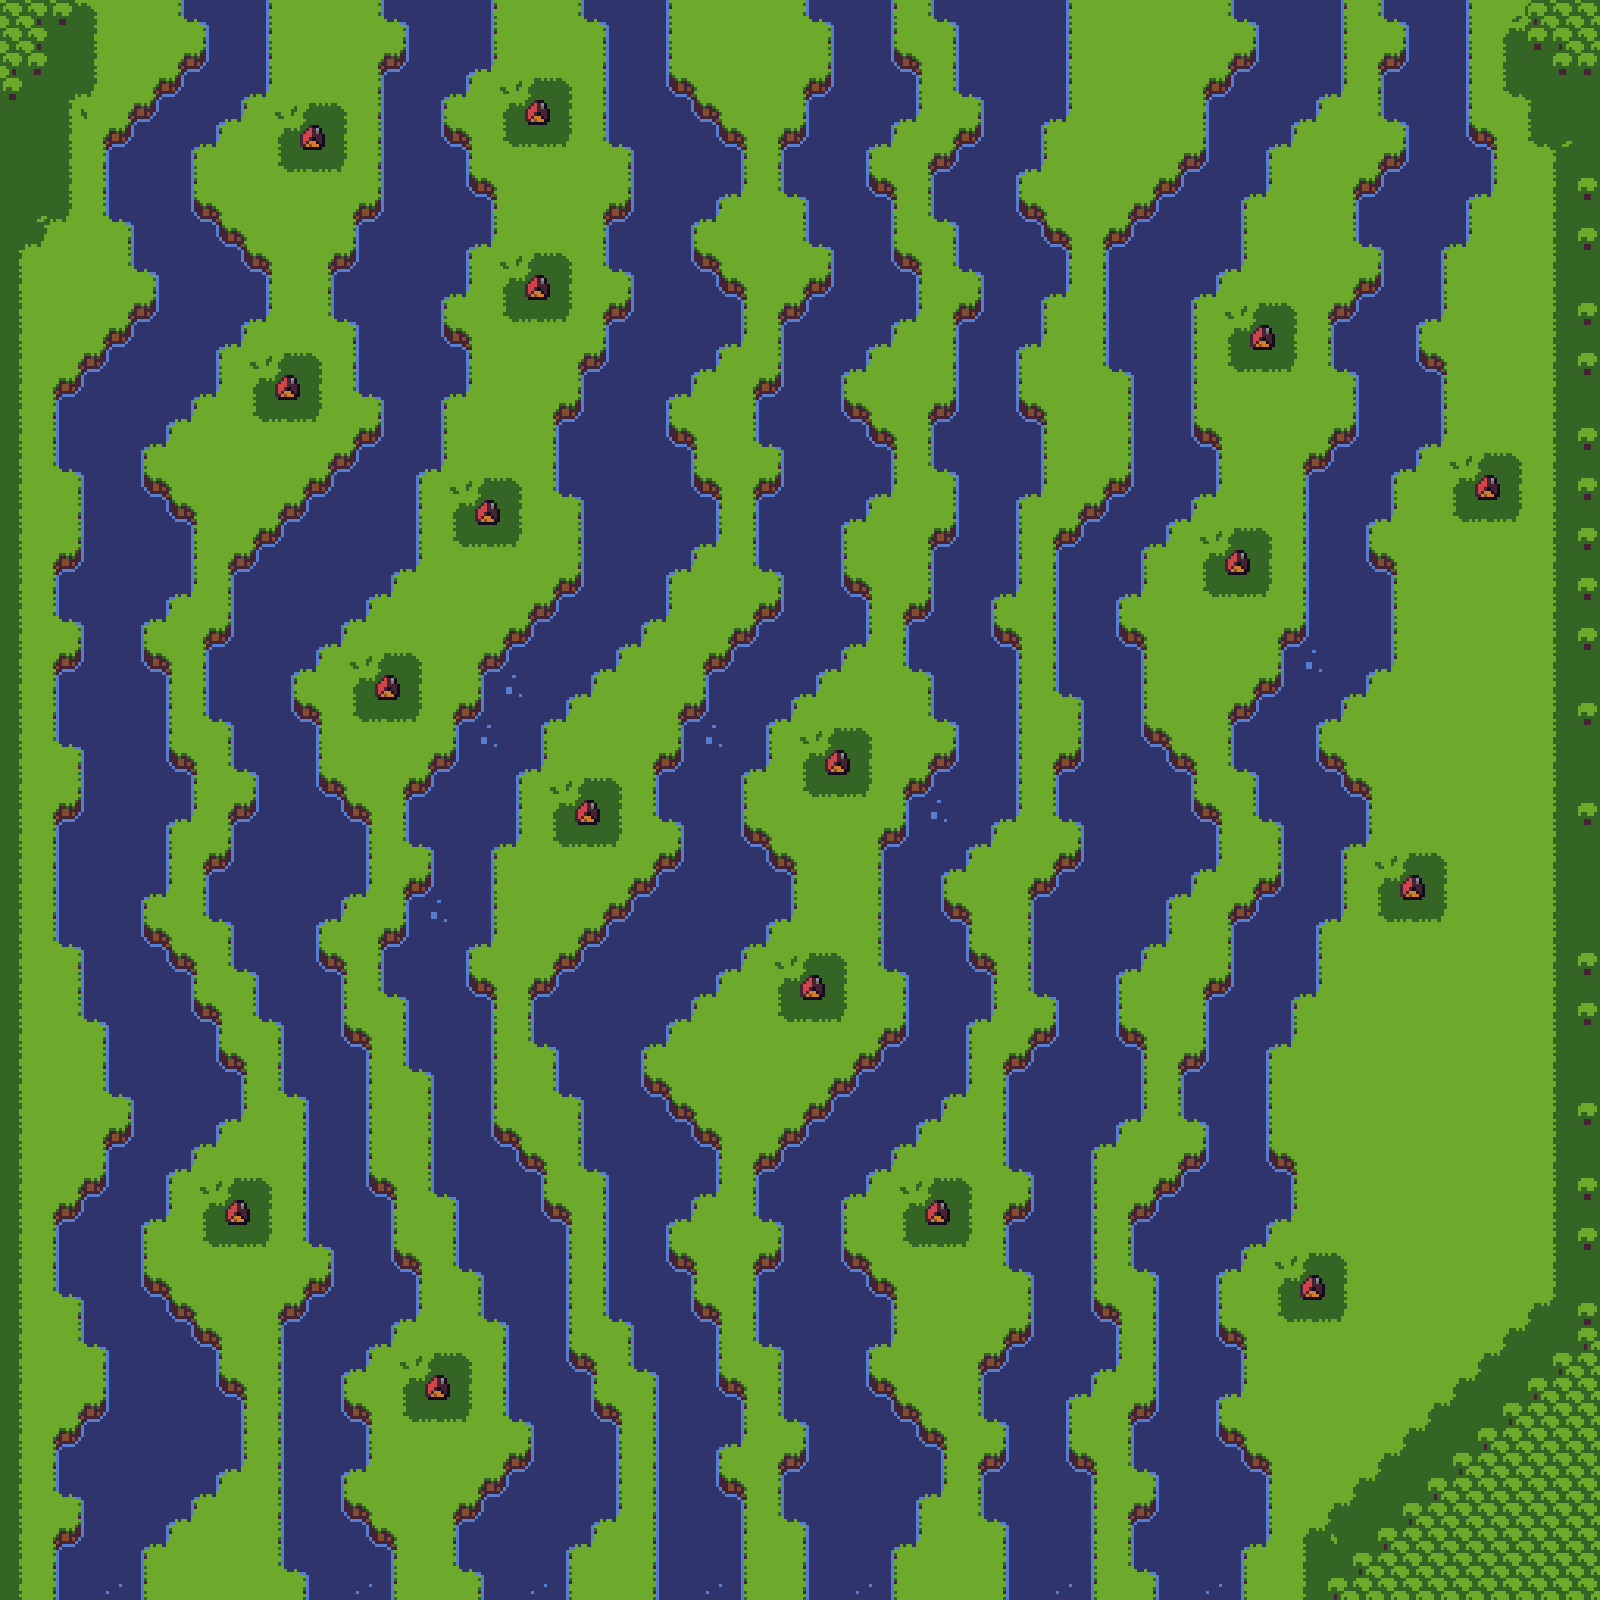
\includegraphics[width=0.9\textwidth]{img/forestmicro_64x64.pdf}
%        \end{block}
%    \end{columns}
%  \end{frame}

  \begin{frame}[fragile]{Introduction}
    Constraint Based Tiling Generation (\textit{CBTG}) Problem
    \begin{columns}[T,onlytextwidth]
      \column{0.5\textwidth}
        \begin{block}{}
          \hfill \\
          \textbf{Find a valid grid realization}

          \begin{itemize}
            \item A \textit{realization} is a single \textit{tile} placement at each \textit{cell} respecting \textit{constraints}.
            \item A \textit{contradiction} if no tiles left at a cell location
          \end{itemize}
        \end{block}
      \column{0.5\textwidth}
        \begin{block}{Example}
          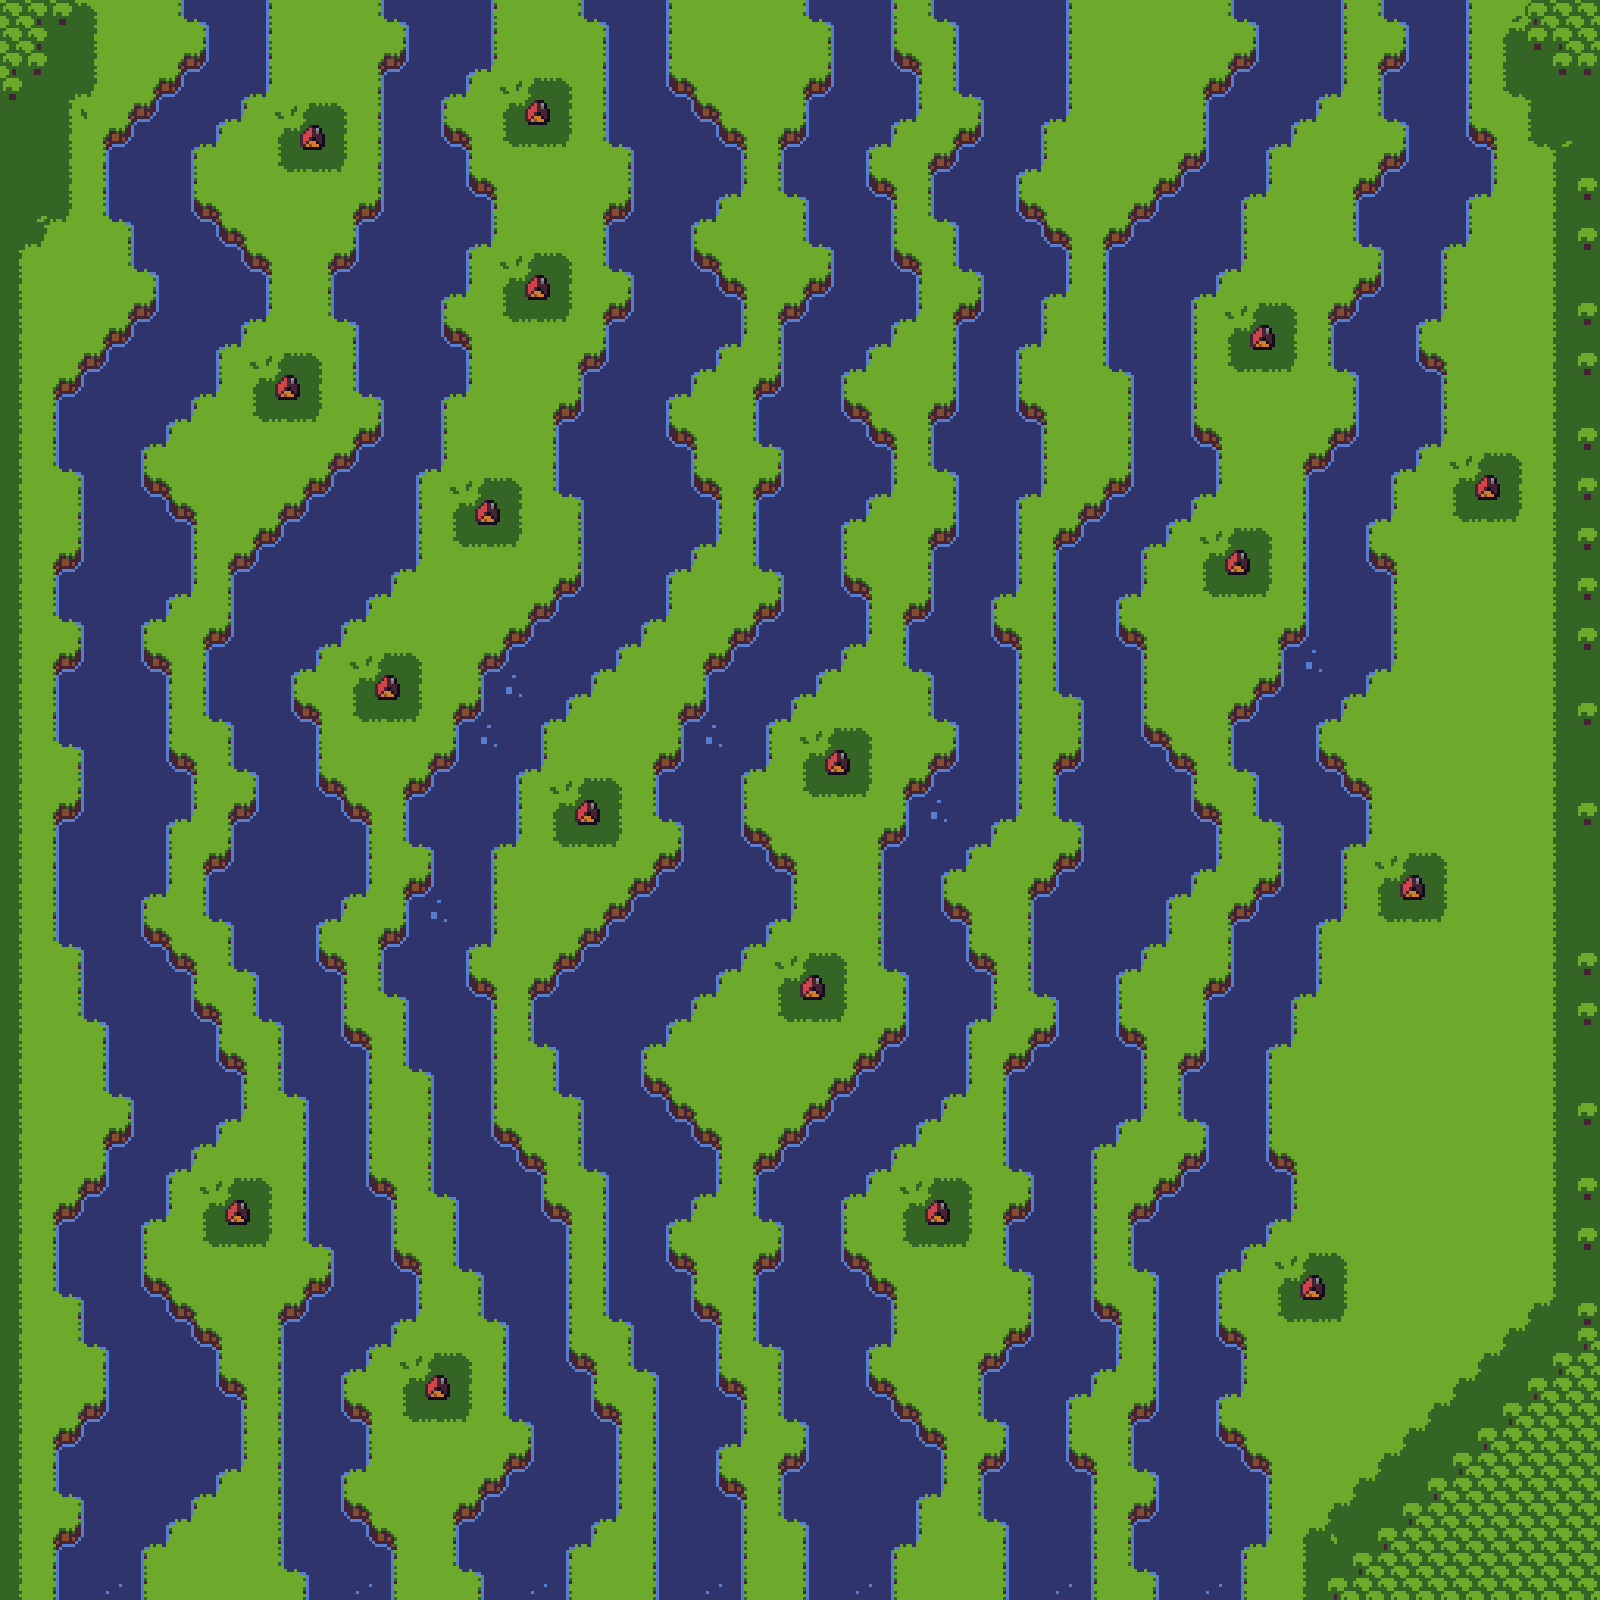
\includegraphics[width=0.9\textwidth]{img/forestmicro_64x64.pdf}
        \end{block}
    \end{columns}
  \end{frame}


  \begin{frame}[fragile]{Introduction}
    \begin{columns}[T,onlytextwidth]
      \column{0.5\textwidth}
        \begin{block}{Definitions}
          \hfill \\
          \begin{itemize}
            \item A tile has \textit{support} if \\
              there's a valid neighbor
              in each
              grid dimension direction
            \item A region is \textit{Arc Consistent} \\ if all \textit{tiles} within the region are \textit{supported}
          \end{itemize}
        \end{block}
      \column{0.5\textwidth}
        \begin{block}{Example}
          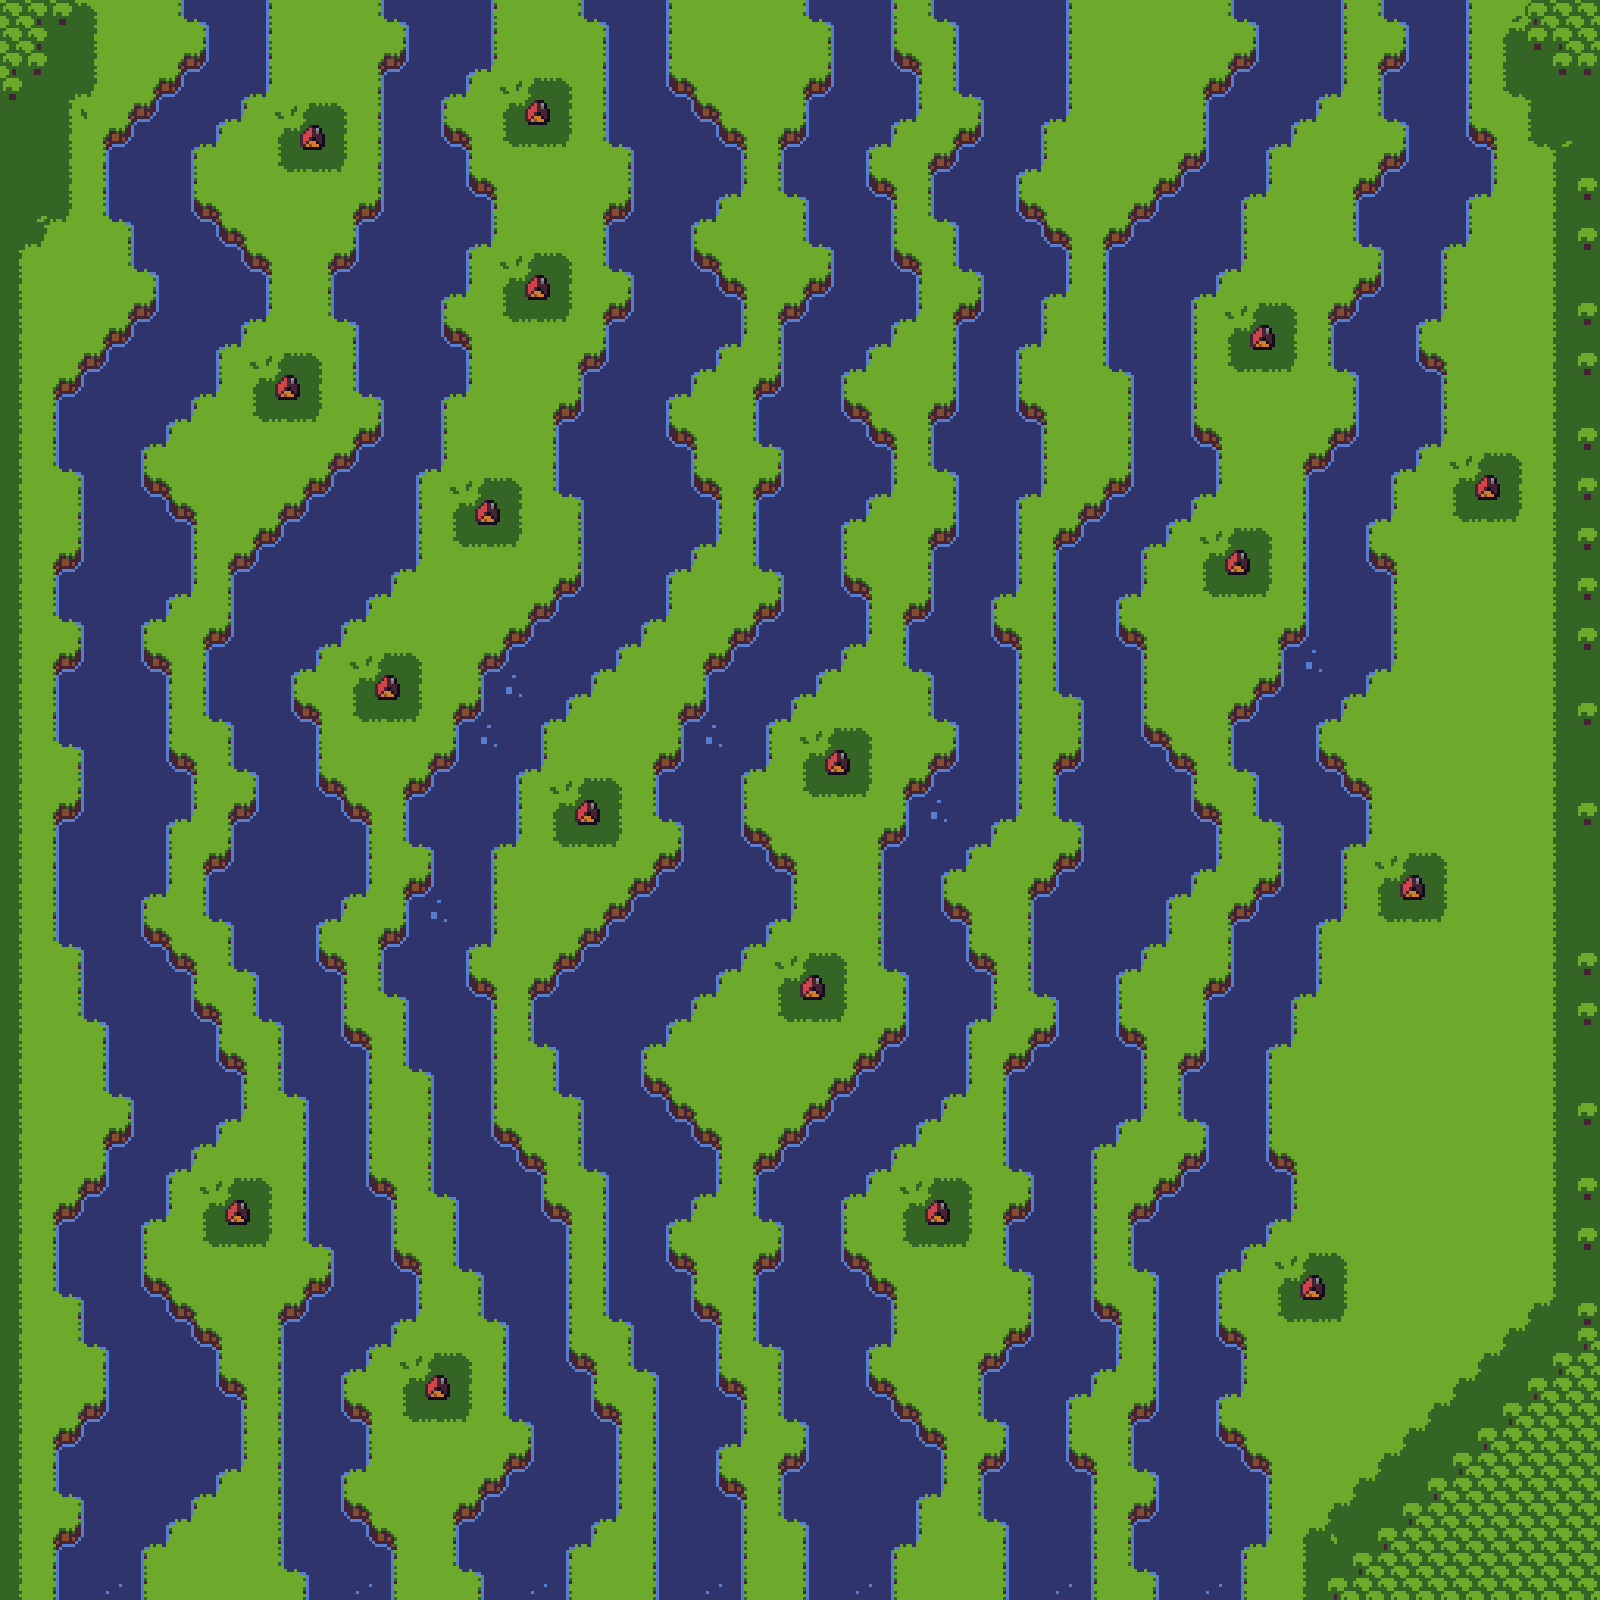
\includegraphics[width=0.9\textwidth]{img/forestmicro_64x64.pdf}
        \end{block}
    \end{columns}
  \end{frame}


  \begin{frame}[fragile]{Introduction}
    \begin{columns}[T,onlytextwidth]
      \column{0.5\textwidth}
        \begin{block}{Definitions}
          \hfill \\
          The basis for a \textit{Constraint Propagation} algorithm
          can be made by removing \textit{unsupported tiles} from
          a \textit{cell's domain}
        \end{block}
      \column{0.5\textwidth}
        \begin{block}{Example}
          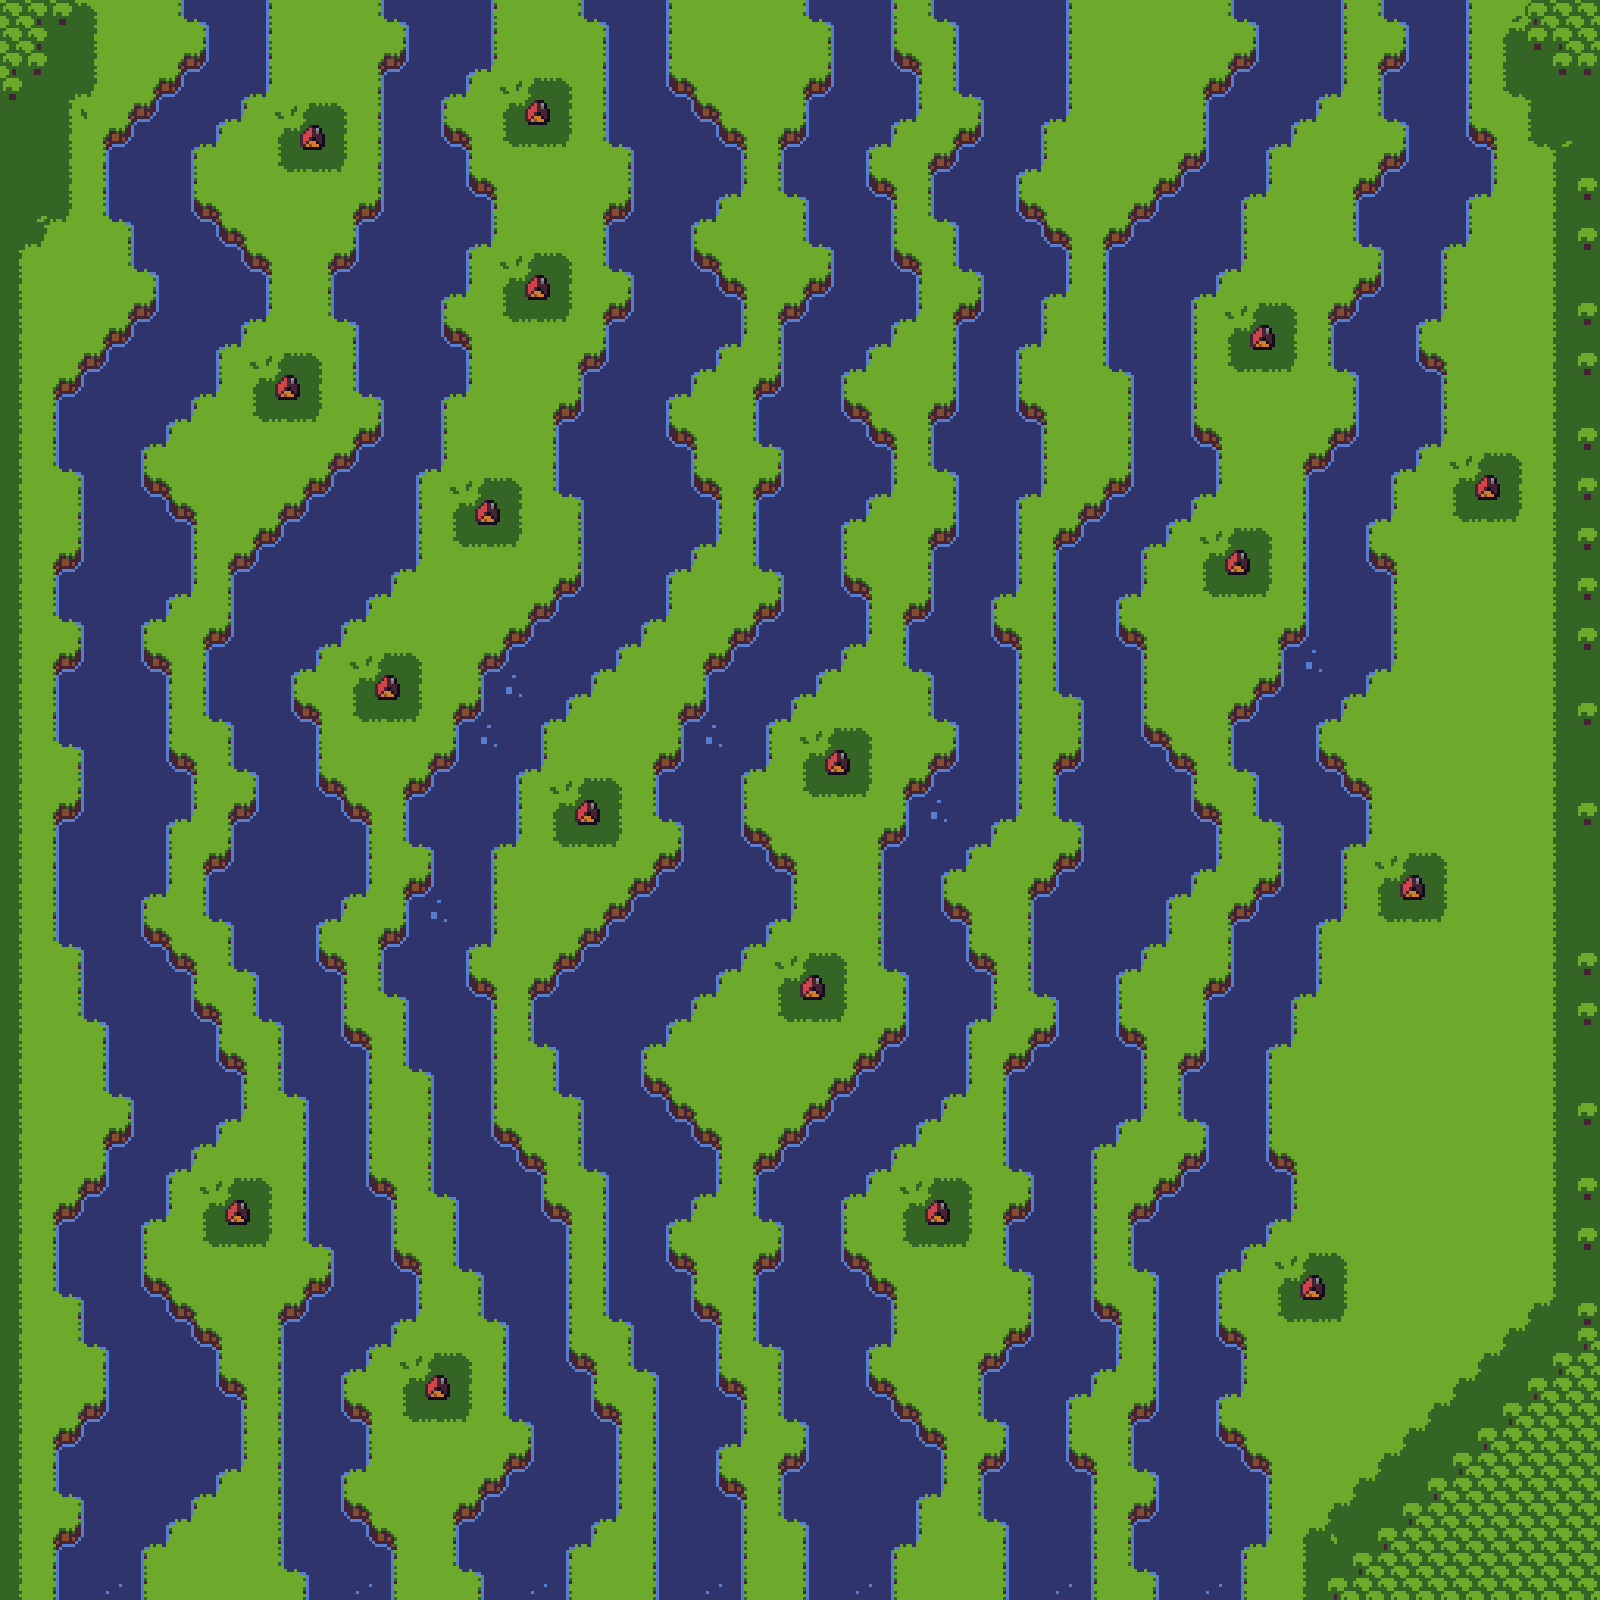
\includegraphics[width=0.9\textwidth]{img/forestmicro_64x64.pdf}
        \end{block}
    \end{columns}
  \end{frame}


%  \begin{frame}[fragile]{Introduction}
%    \begin{columns}[T,onlytextwidth]
%      \column{0.5\textwidth}
%        \begin{block}{Definitions}
%          \hfill \\
%          One such algorithm is \textit{AC4}, which maintains a data
%          structure to count the \textit{support} of each \textit{tile}
%          in each dimension direction
%        \end{block}
%      \column{0.5\textwidth}
%        \begin{block}{Example}
%          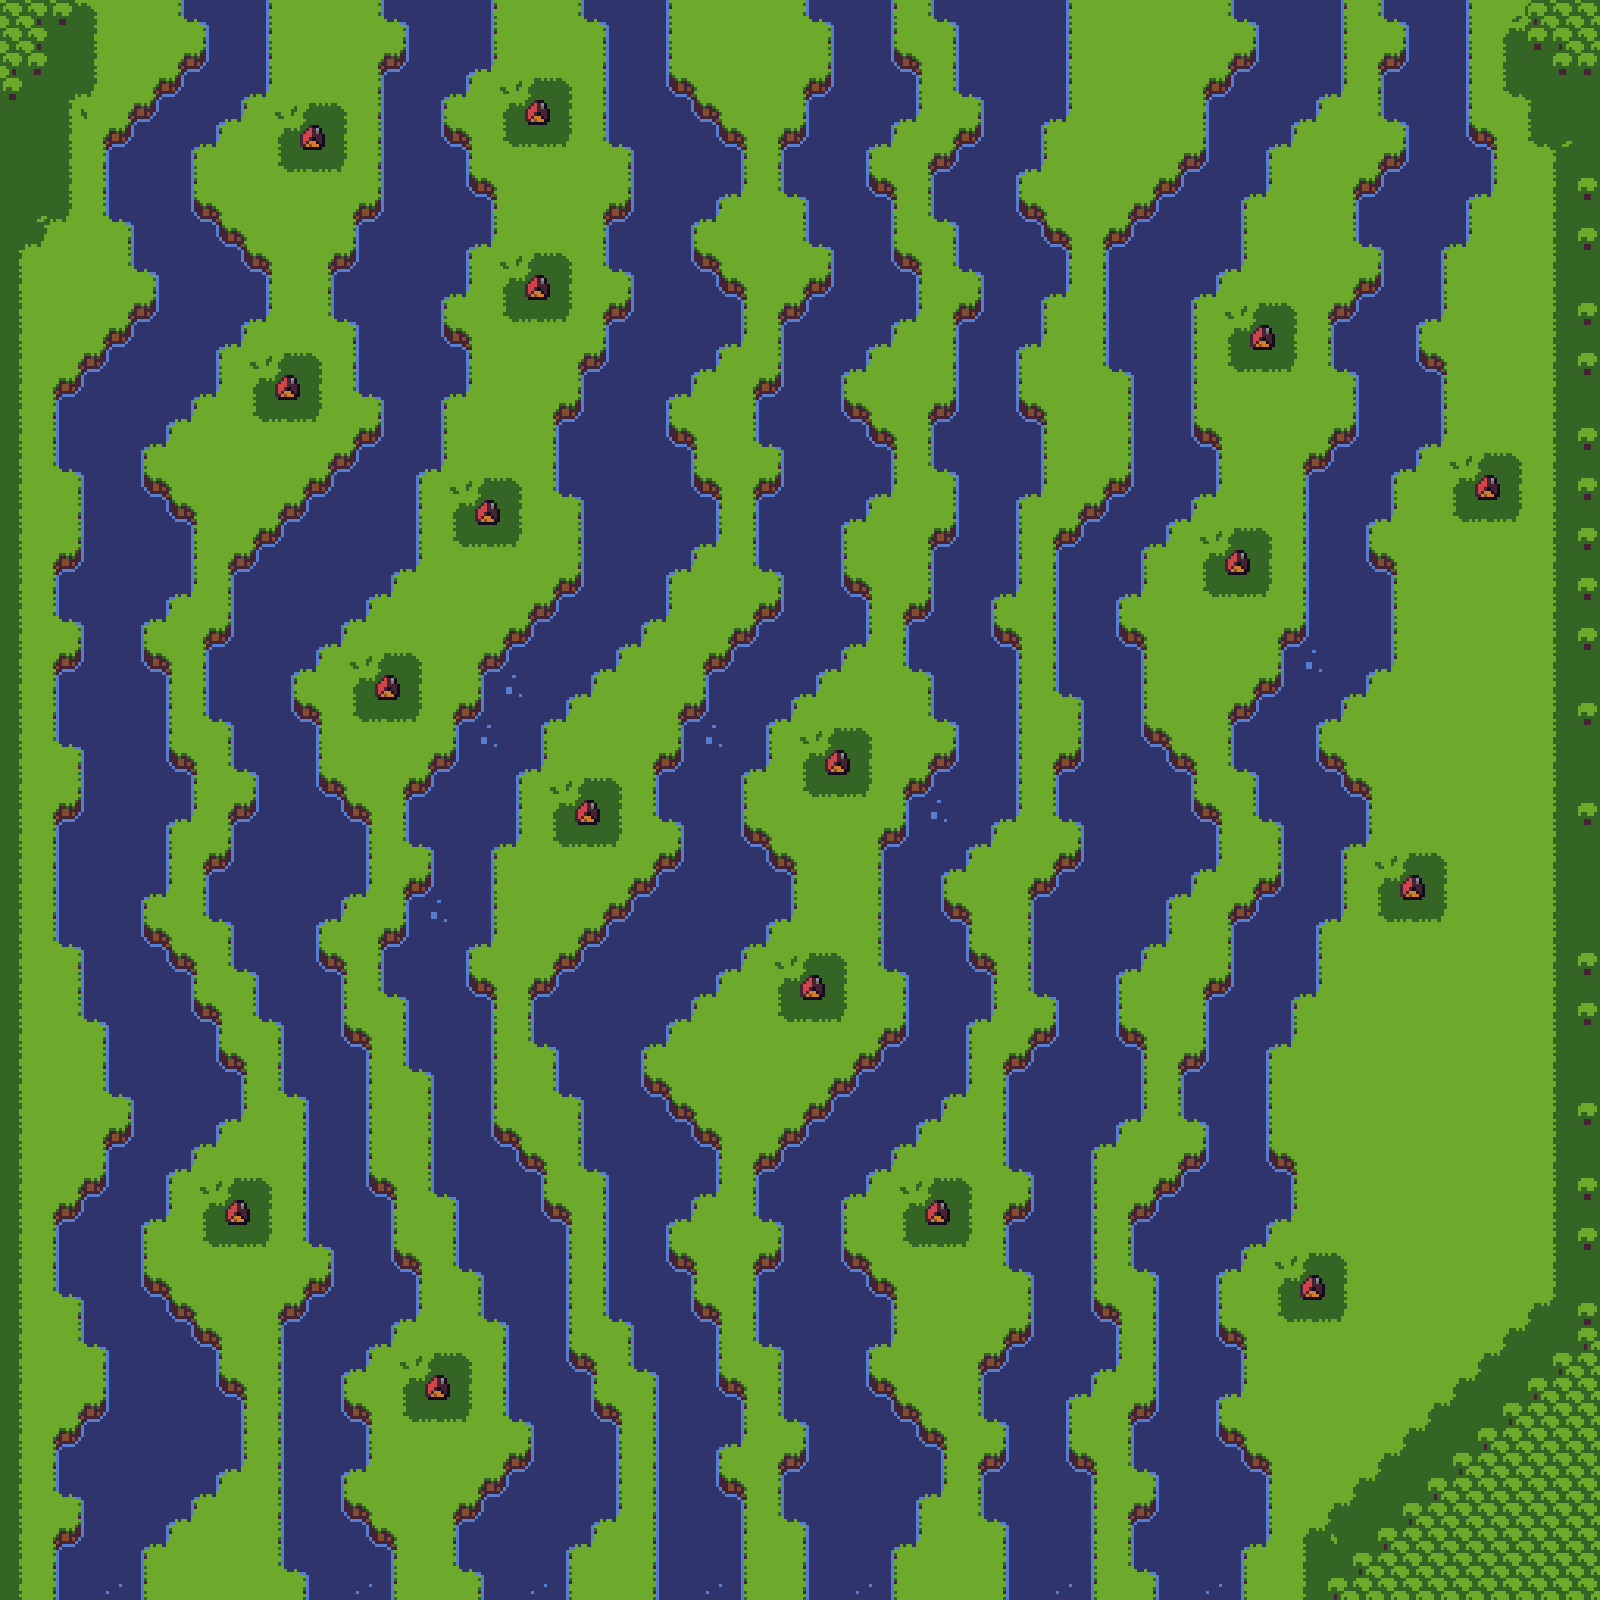
\includegraphics[width=0.9\textwidth]{img/forestmicro_64x64.pdf}
%        \end{block}
%    \end{columns}
%  \end{frame}

%  \begin{frame}[fragile]{Introduction}
%    %\textit{Block} and \textit{Grid} level solvers
%    \begin{columns}[T,onlytextwidth]
%      \column{0.5\textwidth}
%        \begin{block}{Definitions}
%          \hfill \\
%          \begin{itemize}
%            \item \textit{Block Level Solver}: \\
%              completely maintains \textit{Arc Consistency}
%          \end{itemize}
%        \end{block}
%      \column{0.5\textwidth}
%        \begin{block}{Example}
%          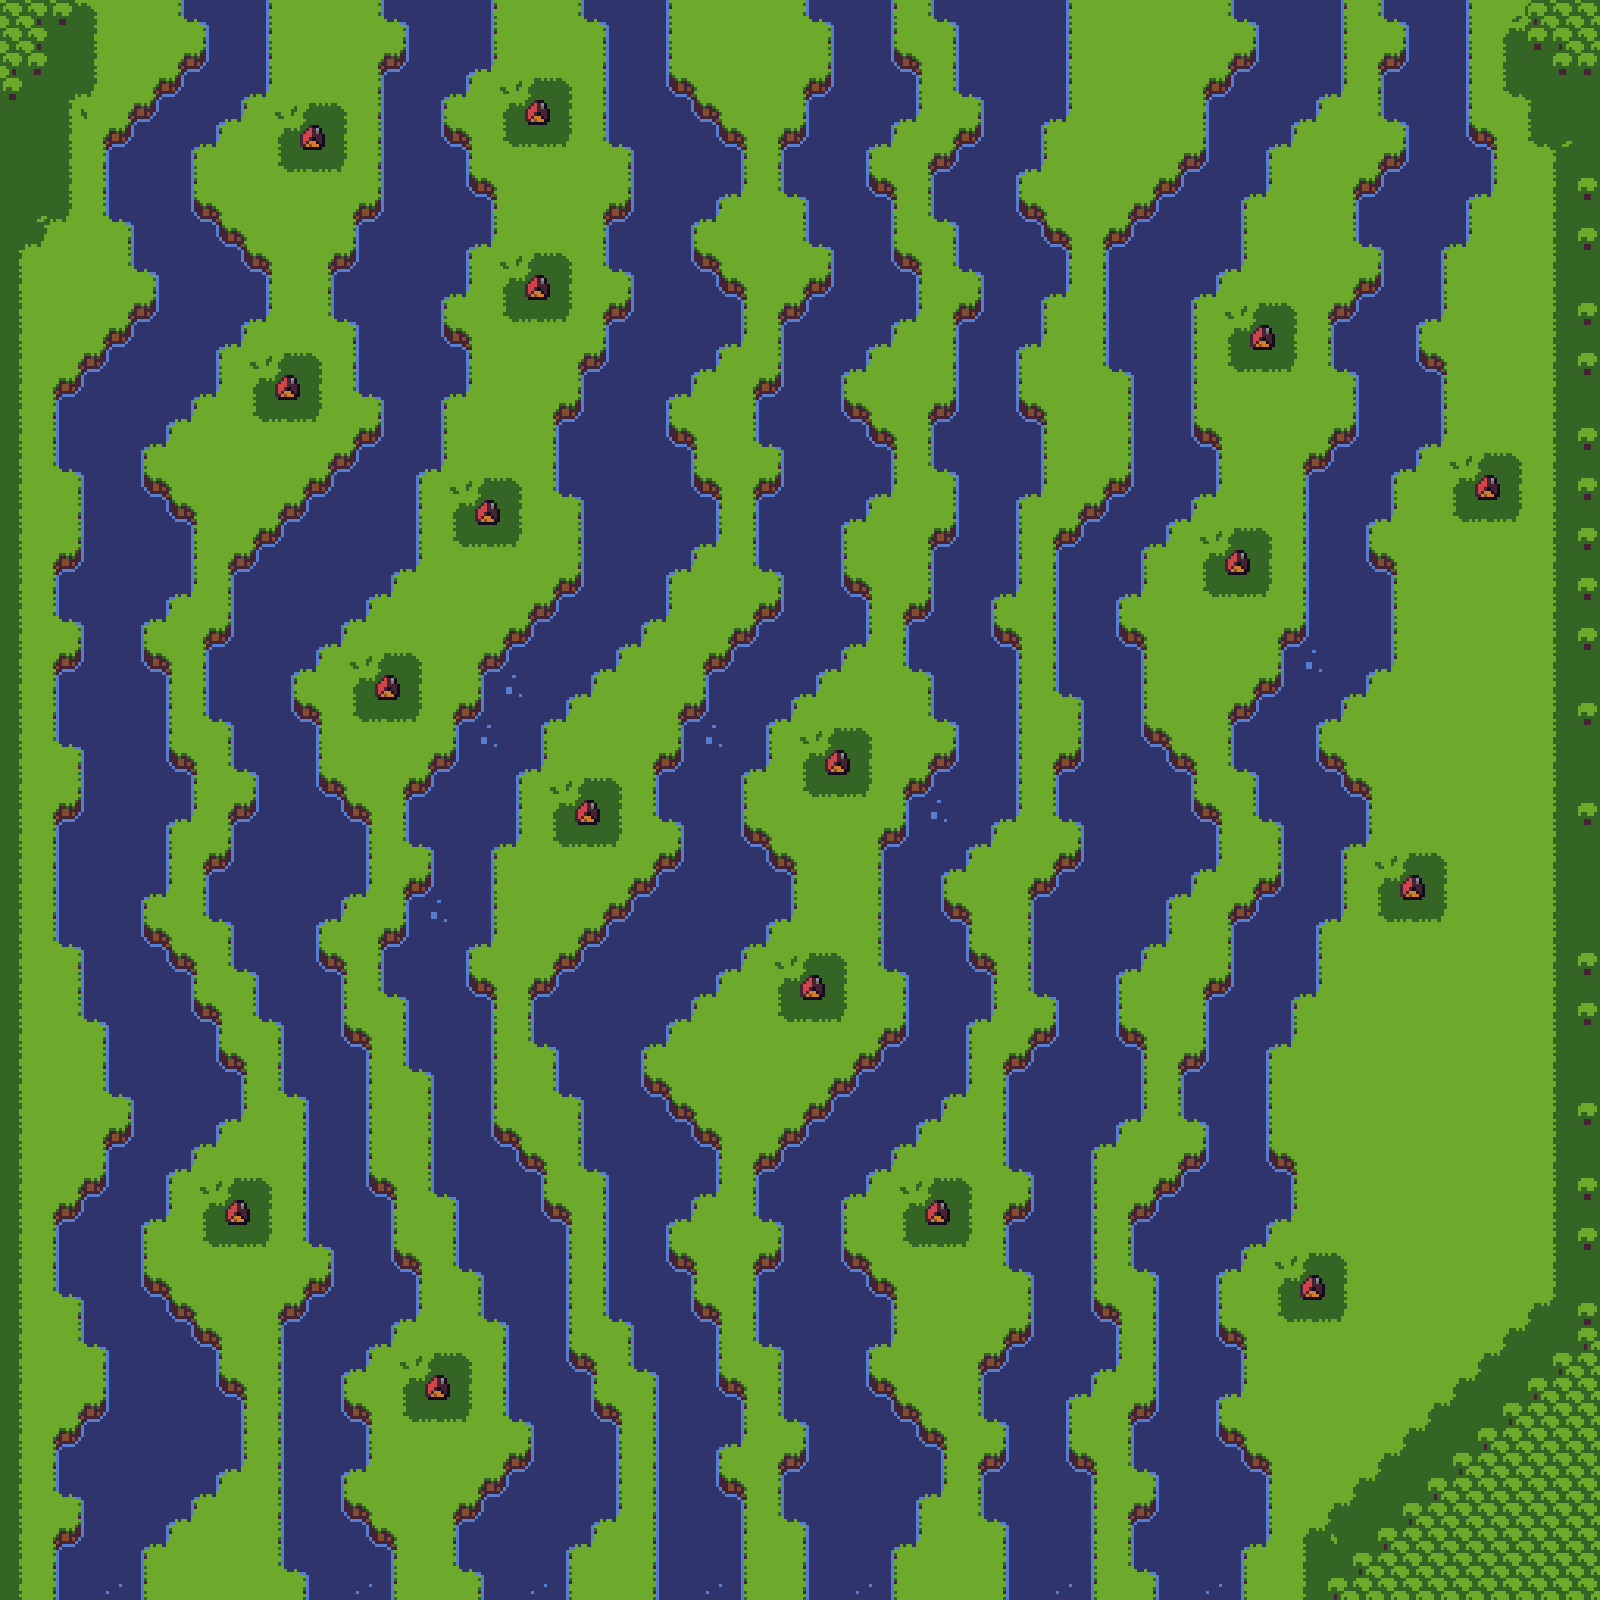
\includegraphics[width=0.9\textwidth]{img/forestmicro_64x64.pdf}
%        \end{block}
%    \end{columns}
%  \end{frame}

  \begin{frame}[fragile]{Introduction}
    %\textit{Block} and \textit{Grid} level solvers
    \begin{columns}[T,onlytextwidth]
      \column{0.5\textwidth}
        \begin{block}{Definitions}
          \hfill \\
          \begin{itemize}
            \item \textit{Block Level Solver}: \\
              completely maintains \textit{Arc Consistency}
            \item \textit{Grid Level Solver}: \\
              only keep summary information for the entire grid but
              work on \textit{block} sub-regions
          \end{itemize}
        \end{block}
      \column{0.5\textwidth}
        \begin{block}{Example}
          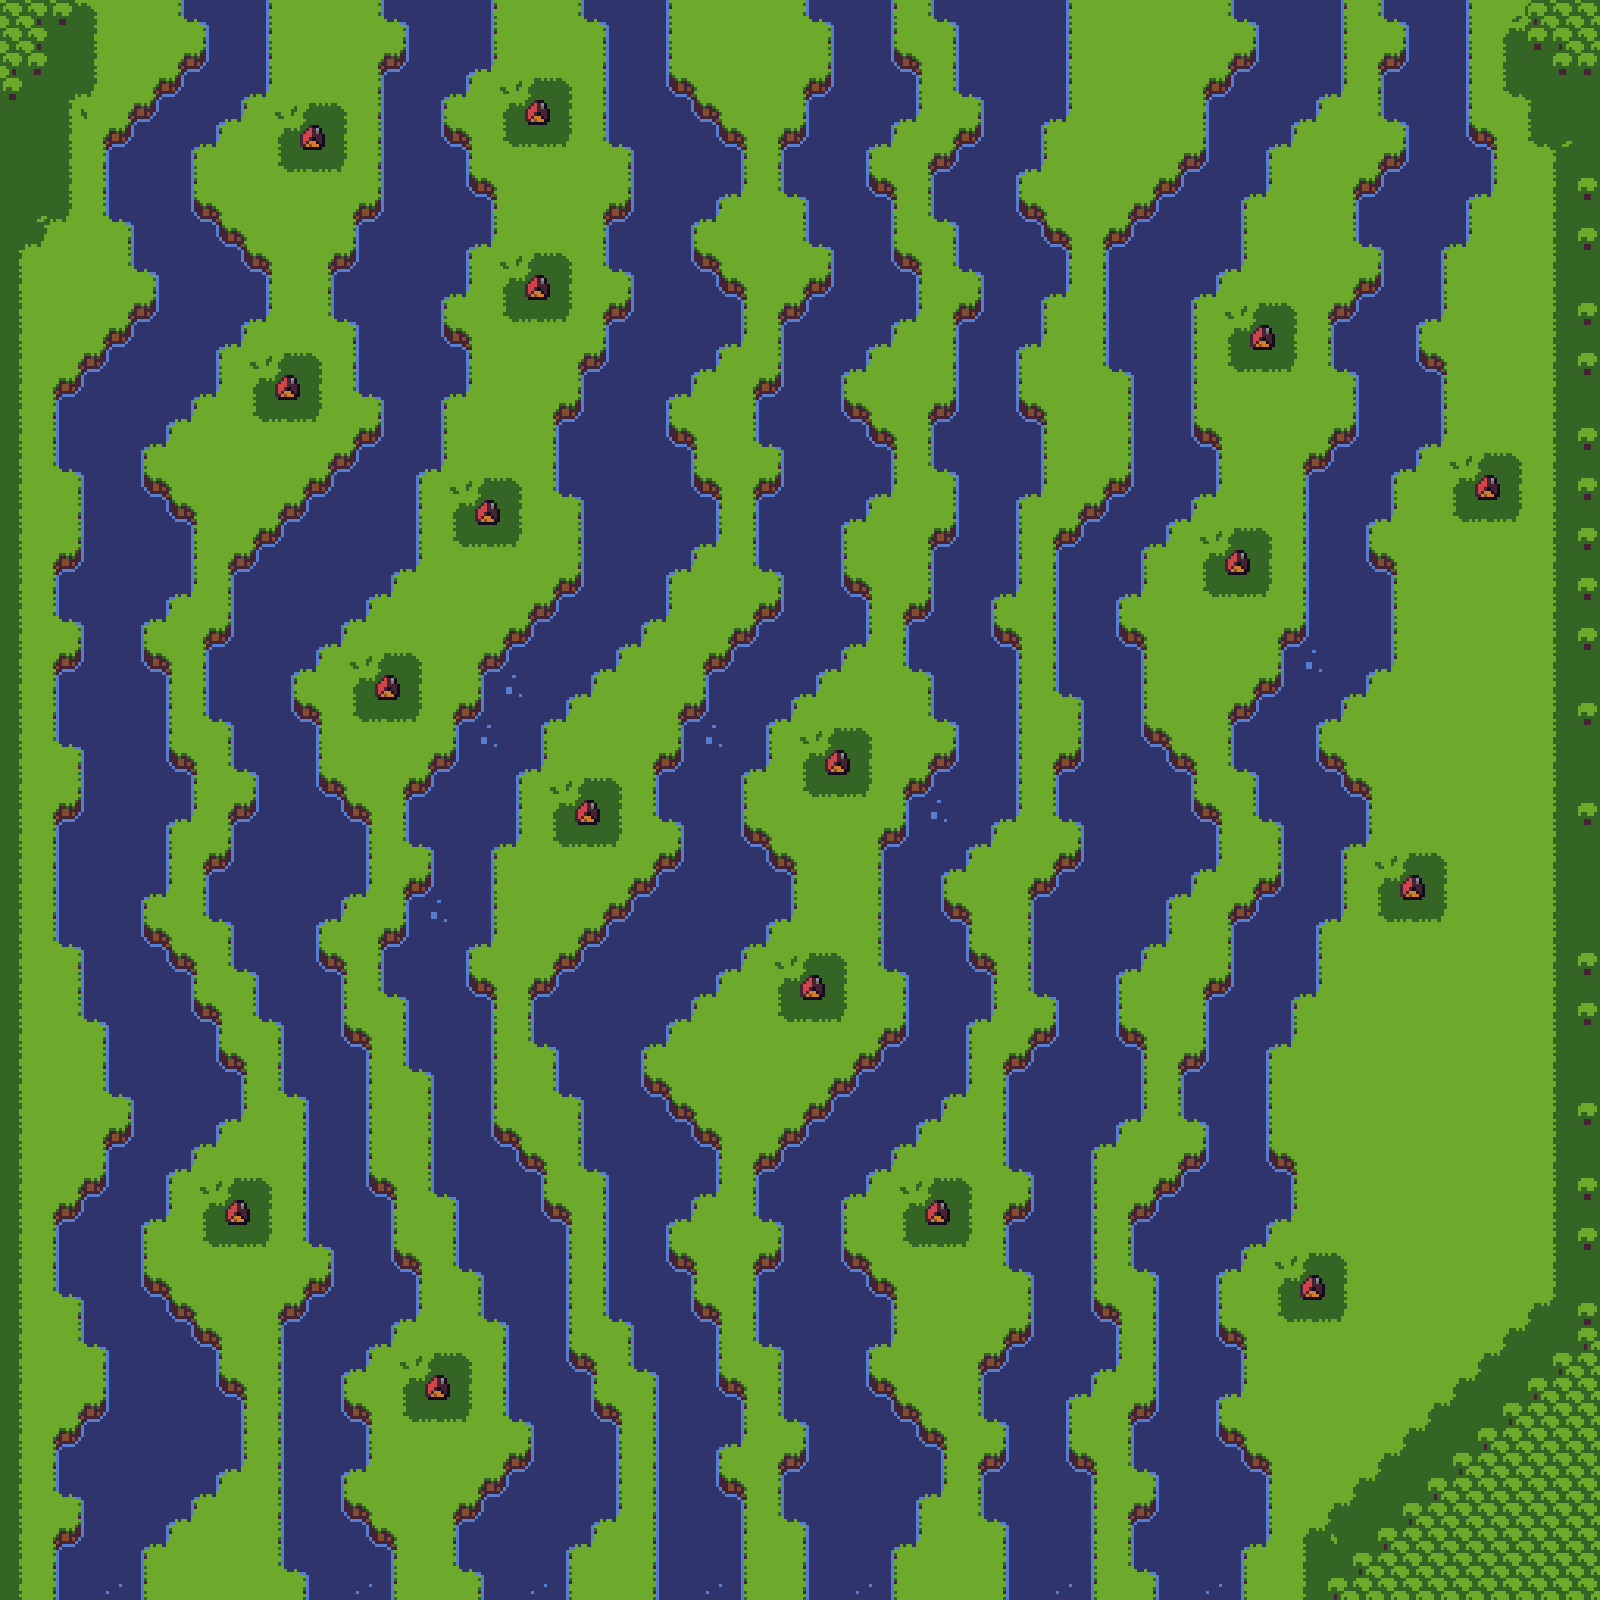
\includegraphics[width=0.9\textwidth]{img/forestmicro_64x64.pdf}
        \end{block}
    \end{columns}
  \end{frame}


  %%%%%%%%%%%%%%
  %%%%%%%%%%%%%%
  %%%%%%%%%%%%%%
  
  %\section{Related Work}

  \begin{frame}[fragile]{Related Work}
    WFC, BMS, MMS

    \begin{itemize}
      \item Gumin's \textit{Wave Function Collapse} (\textit{WFC})
      \item \textit{Breakout Model Synthesis} (\textit{BMS}) \\
        \ \ \ (Hoetzlein's \textit{just\_math} project)
      \item Merrell's \textit{Modify in Blocks Model Synthesis} (\textit{MMS})
    \end{itemize}
  \end{frame}

  %% wfc_related_work

  \begin{frame}[fragile]{Related Work}
    \textit{Wave Function Collapse} (\textit{WFC})
    \begin{columns}[T,onlytextwidth]
      \column{0.5\textwidth}
        \begin{block}{WFC}
          \hfill \\
          \begin{itemize}
            \item Resolve tile at cell (min. entropy heuristic)
            \item Constraint Propagate
            \item Loop until solution or contradiction
          \end{itemize}
        \end{block}
      \column{0.5\textwidth}
        \begin{block}{Example}
          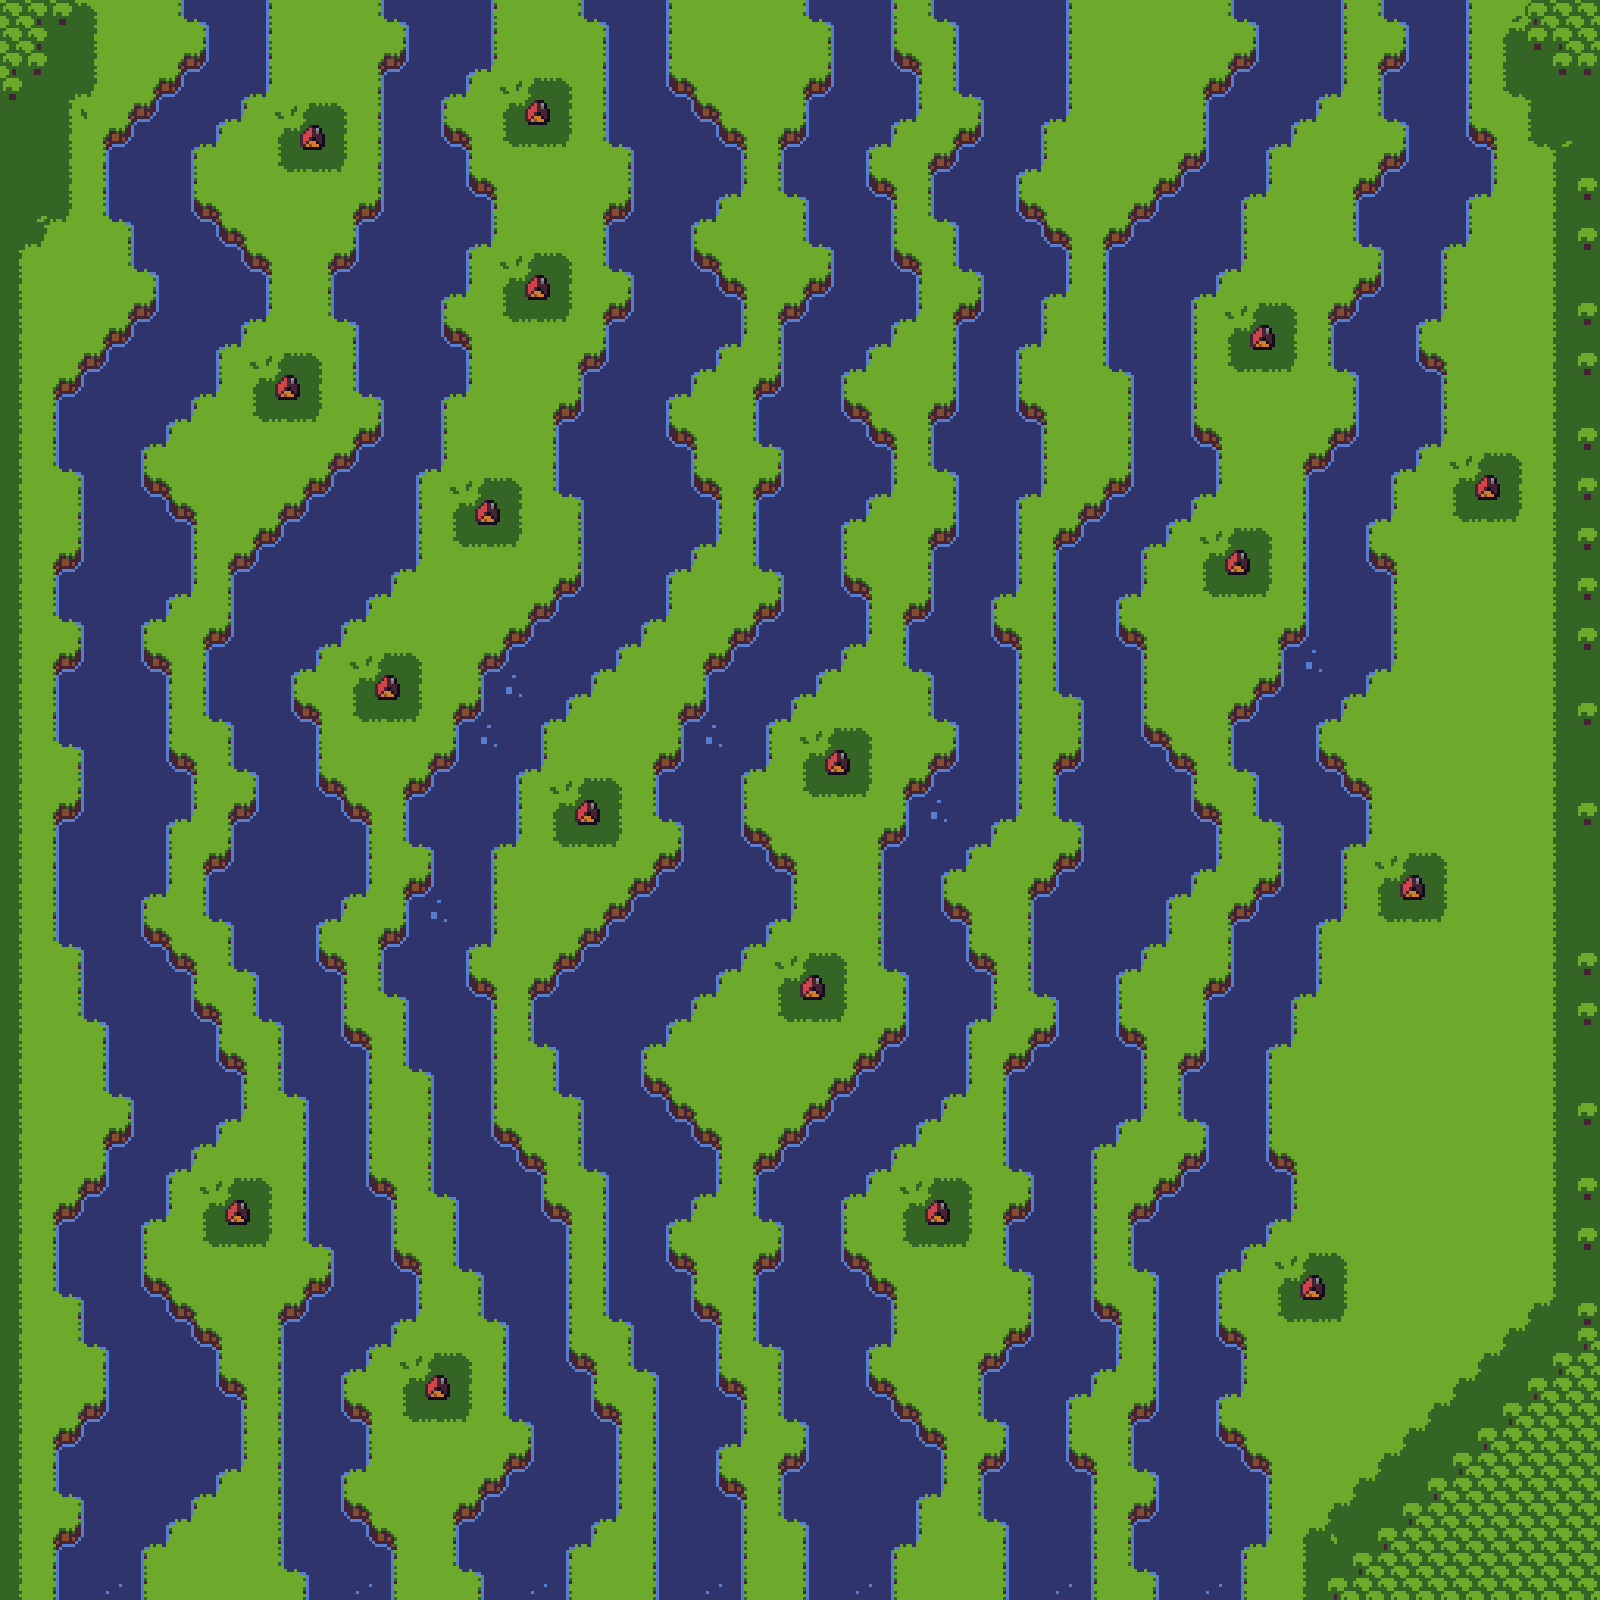
\includegraphics[width=0.9\textwidth]{img/forestmicro_64x64.pdf}
        \end{block}
    \end{columns}
  \end{frame}

  \begin{frame}[fragile]{Related Work}
    \textit{Wave Function Collapse} (\textit{WFC})
    \begin{columns}[T,onlytextwidth]
      \column{0.5\textwidth}
        \begin{block}{WFC}
          \hfill \\
          \begin{itemize}
            \item \textit{Block Level}
            \item One-shot
            \item Indeterminate initial condition
            \item Ergodic
          \end{itemize}
        \end{block}
      \column{0.5\textwidth}
        \begin{block}{Example}
          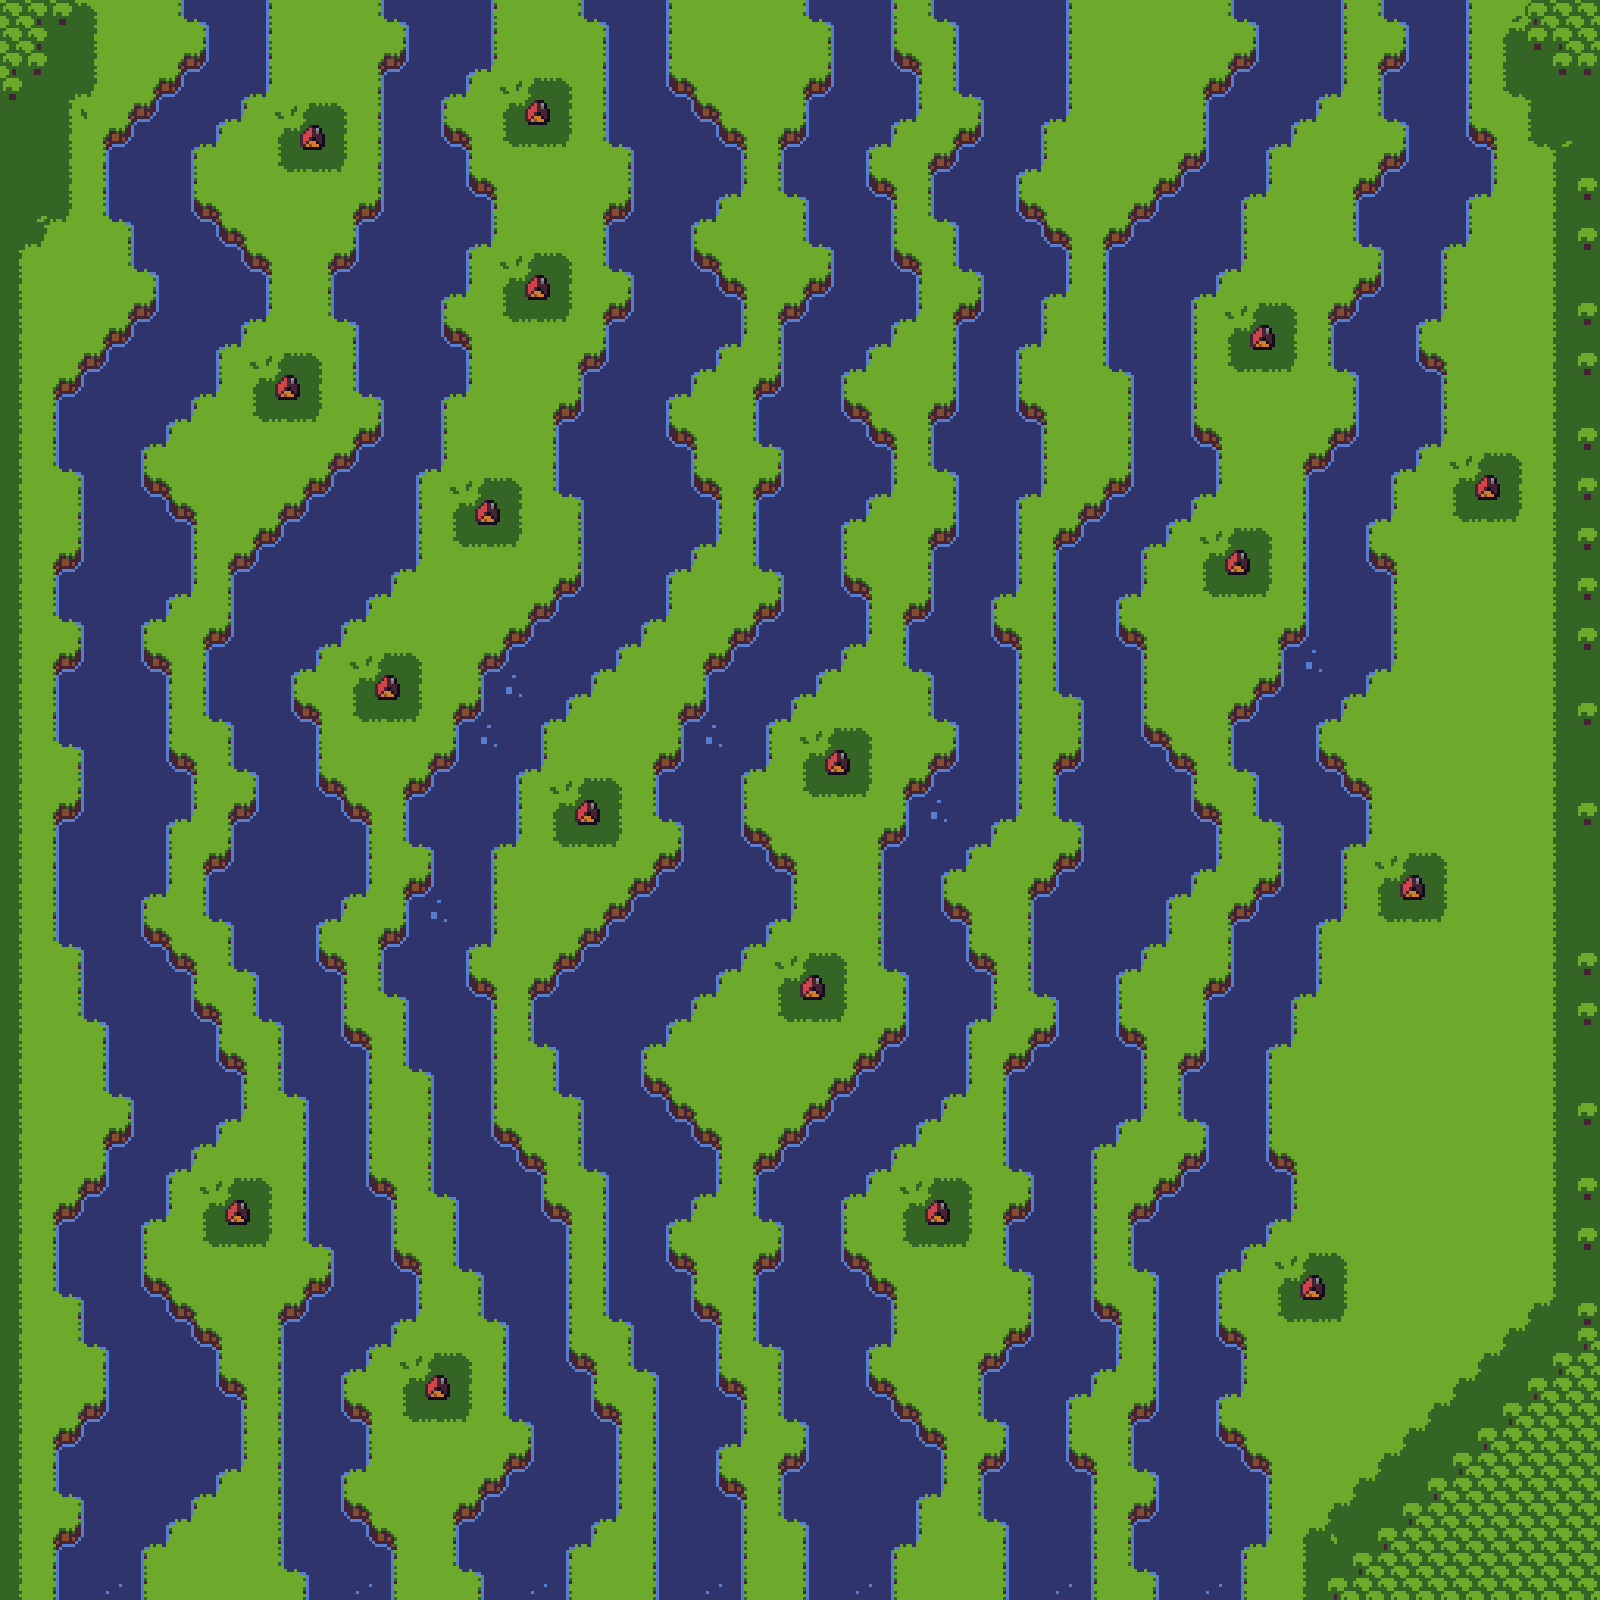
\includegraphics[width=0.9\textwidth]{img/forestmicro_64x64.pdf}
        \end{block}
    \end{columns}
  \end{frame}

  %% bms_related_work

  \begin{frame}[fragile]{Related Work}
    \textit{Breakout Model Synthesis} (\textit{BMS})
    \begin{columns}[T,onlytextwidth]
      \column{0.5\textwidth}
        \begin{block}{BMS}
          \hfill \\
          \begin{itemize}
            \item Resolve tile at cell
            \item Constraint Propagate
            \item If contradiction
              \begin{itemize}
                \item Revert small region
              \end{itemize}
            \item Loop until solution or timeout
          \end{itemize}
        \end{block}
      \column{0.5\textwidth}
        \begin{block}{Example}
          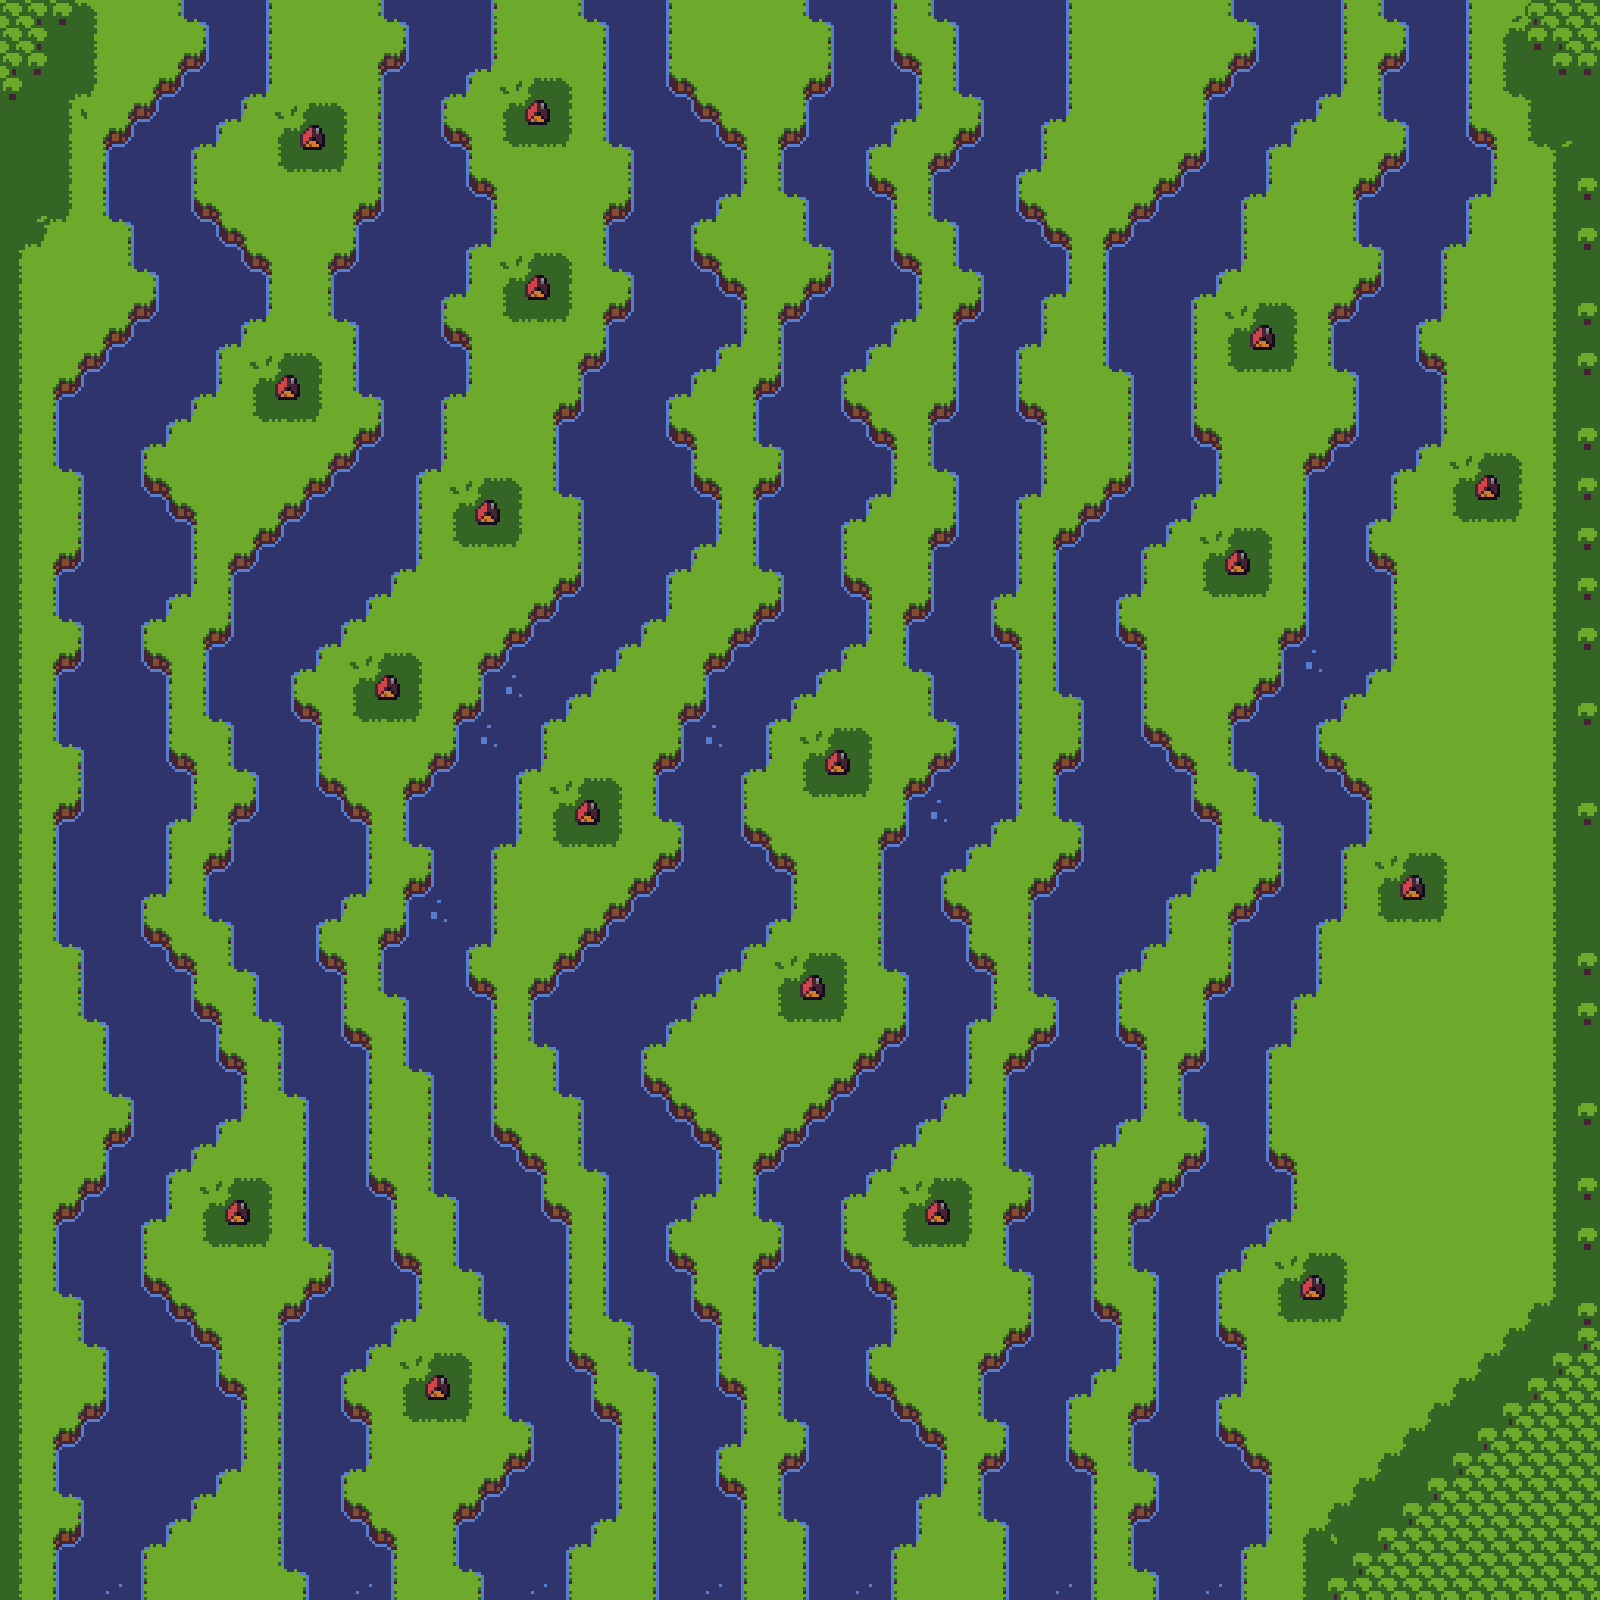
\includegraphics[width=0.9\textwidth]{img/forestmicro_64x64.pdf}
        \end{block}
    \end{columns}
  \end{frame}

  \begin{frame}[fragile]{Related Work}
    \textit{Breakout Model Synthesis} (\textit{BMS})
    \begin{columns}[T,onlytextwidth]
      \column{0.5\textwidth}
        \begin{block}{BMS}
          \hfill \\
          \begin{itemize}
            \item \textit{Block Level}
            \item Stochastic backtracking
            \item Indeterminate initial condition
            \item Ergodic
          \end{itemize}
        \end{block}
      \column{0.5\textwidth}
        \begin{block}{Example}
          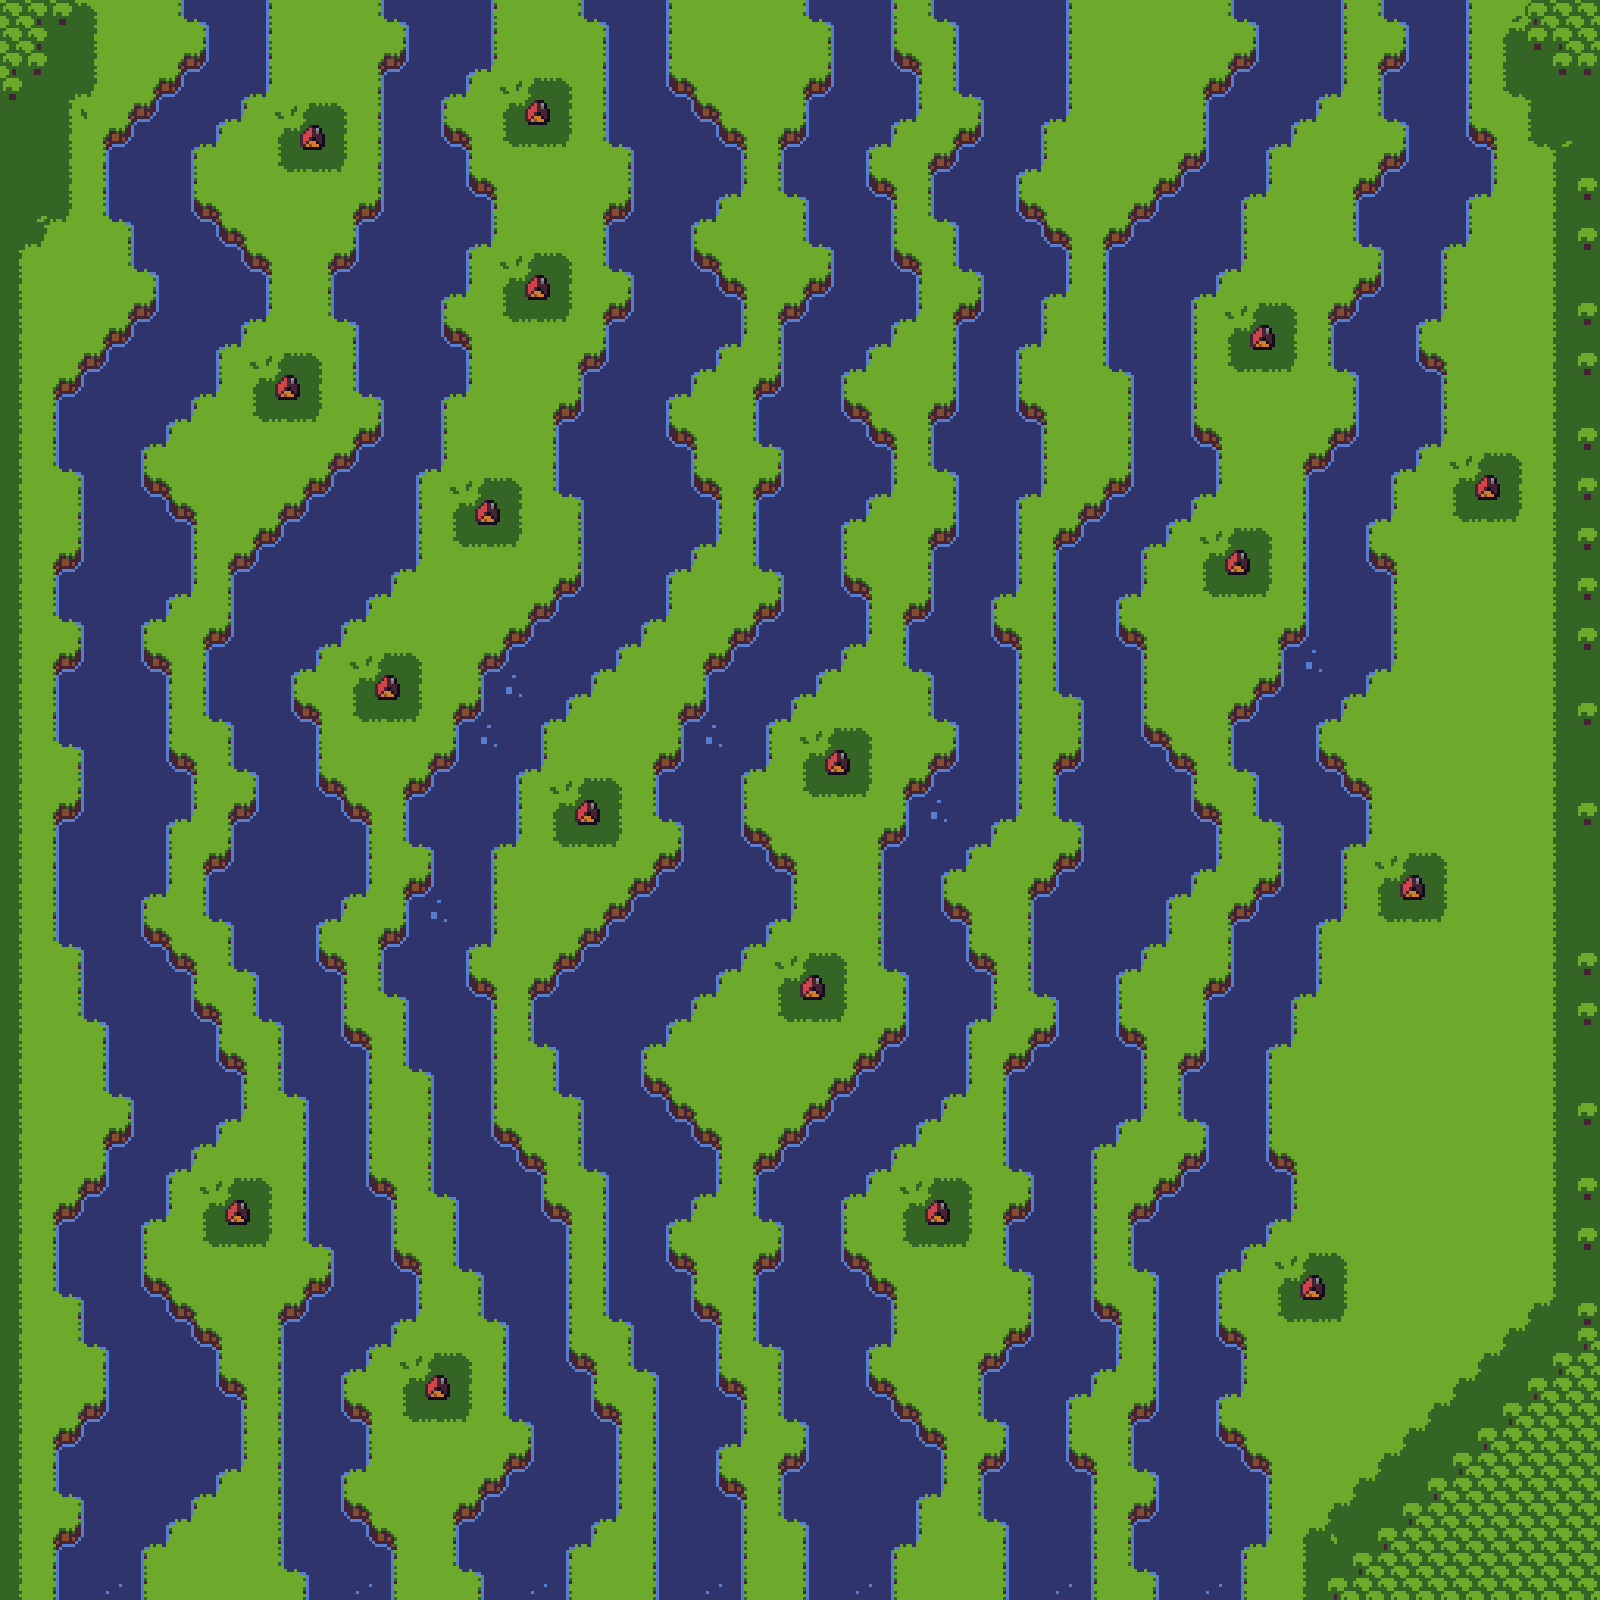
\includegraphics[width=0.9\textwidth]{img/forestmicro_64x64.pdf}
        \end{block}
    \end{columns}
  \end{frame}

  % mms_related_work

  \begin{frame}[fragile]{Related Work}
    \textit{Modify in Blocks Model Synthesis} (\textit{MMS})
    \begin{columns}[T,onlytextwidth]
      \column{0.5\textwidth}
        \begin{block}{MMS}
          \hfill \\
          \begin{itemize}
            \item Start from resolved grid
            \item Choose block
            \item Try to resolve block
            \item If block resolved
              \begin{itemize}
                \item incoporate block
              \end{itemize}
            \item Else restore block
            \item Loop to taste
          \end{itemize}
        \end{block}
      \column{0.5\textwidth}
        \begin{block}{Example}
          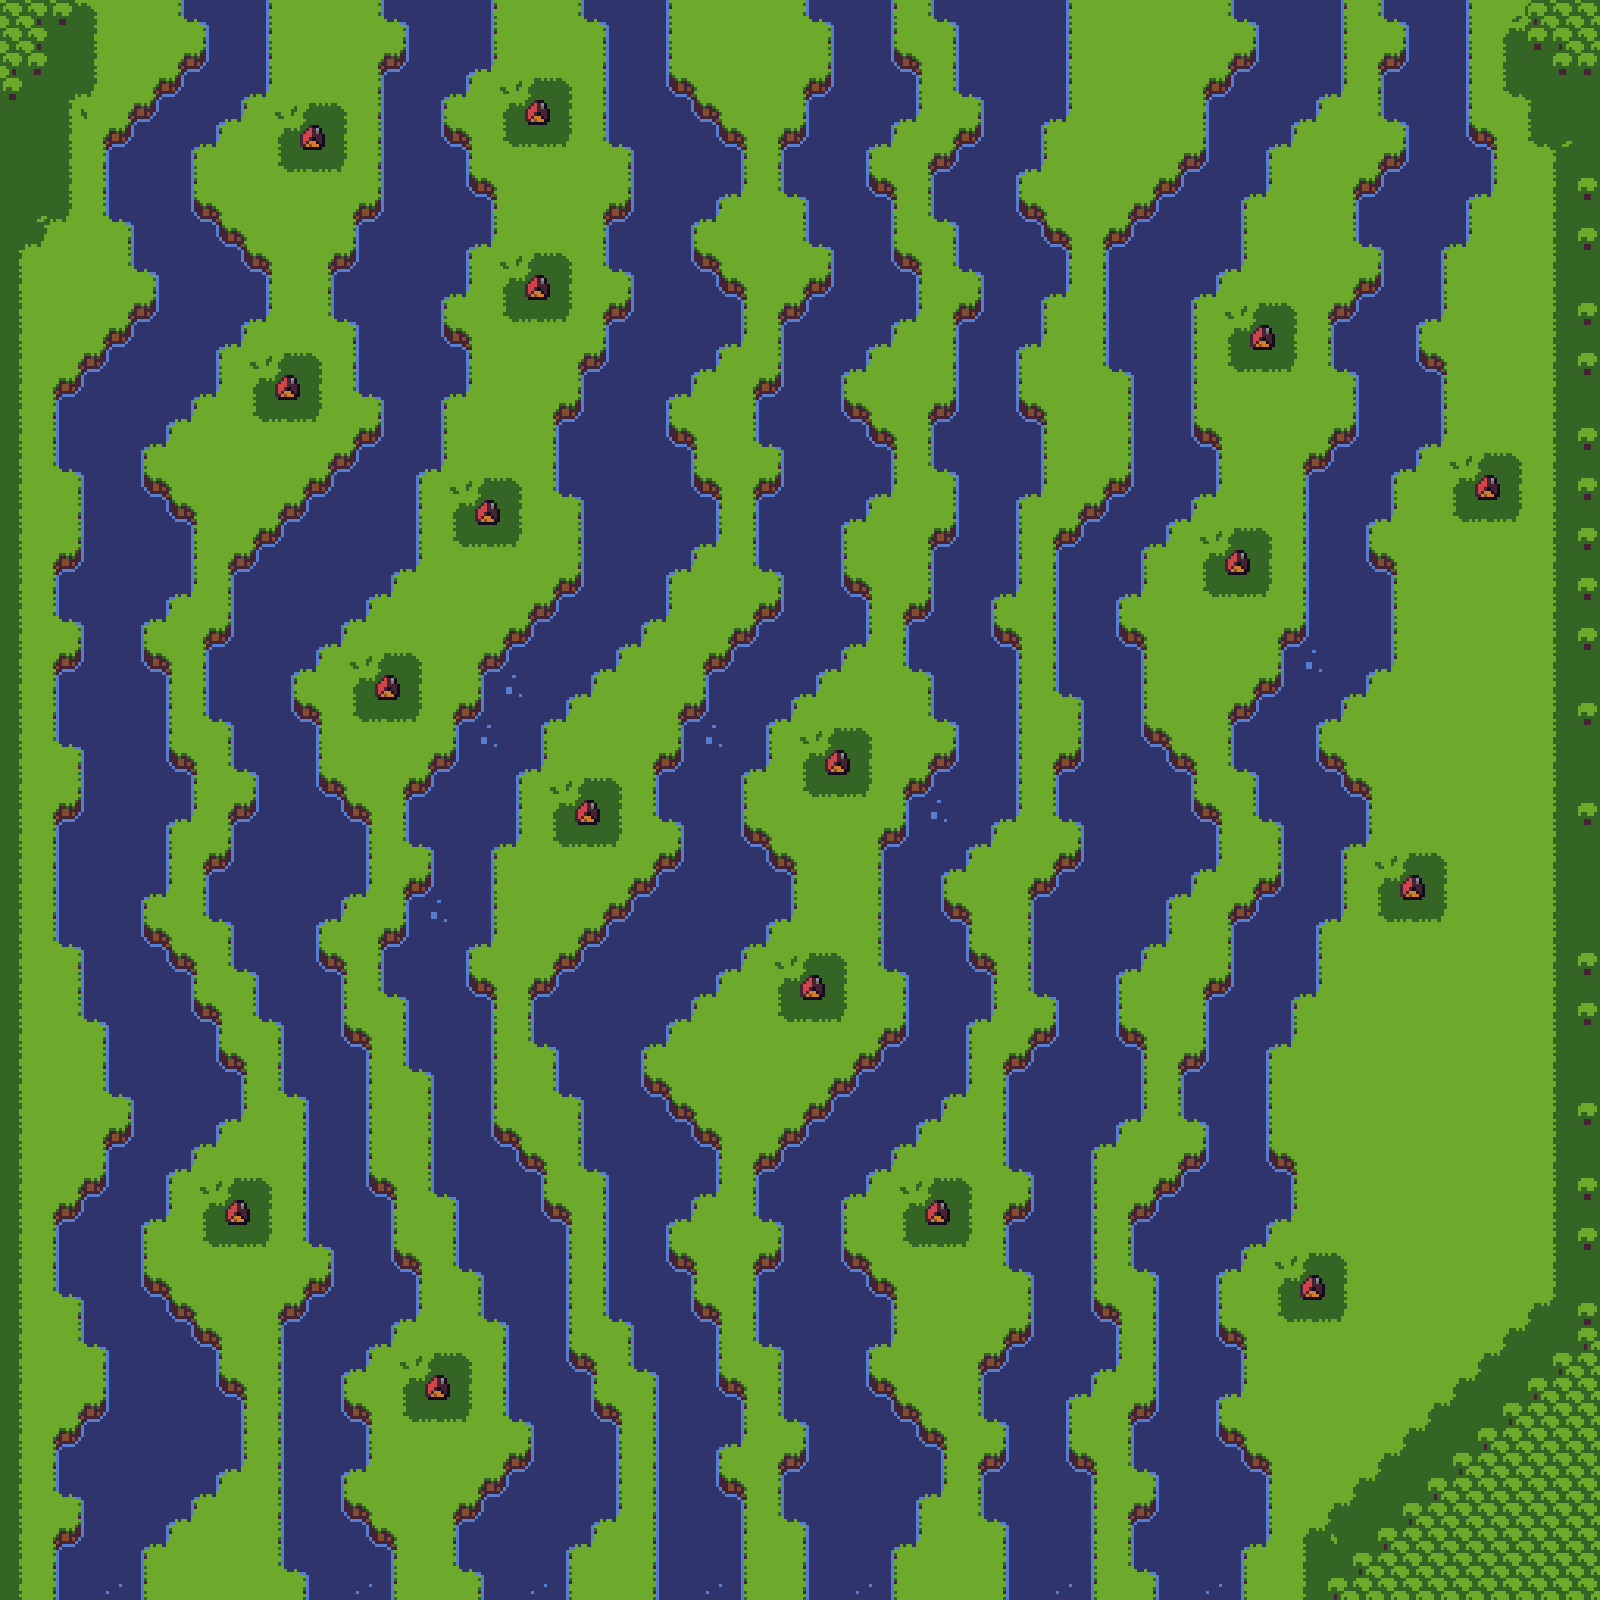
\includegraphics[width=0.9\textwidth]{img/forestmicro_64x64.pdf}
        \end{block}
    \end{columns}
  \end{frame}

  \begin{frame}[fragile]{Related Work}
    \textit{Modify in Blocks Model Synthesis} (\textit{MMS})
    \begin{columns}[T,onlytextwidth]
      \column{0.5\textwidth}
        \begin{block}{MMS}
          \hfill \\
          \begin{itemize}
            \item \textit{Grid Level}
            \item Contradiction resilience via
              Block step consistency
            \item Requires bootstrap initial realization
            \item Non-ergodic
          \end{itemize}
        \end{block}
      \column{0.5\textwidth}
        \begin{block}{Example}
          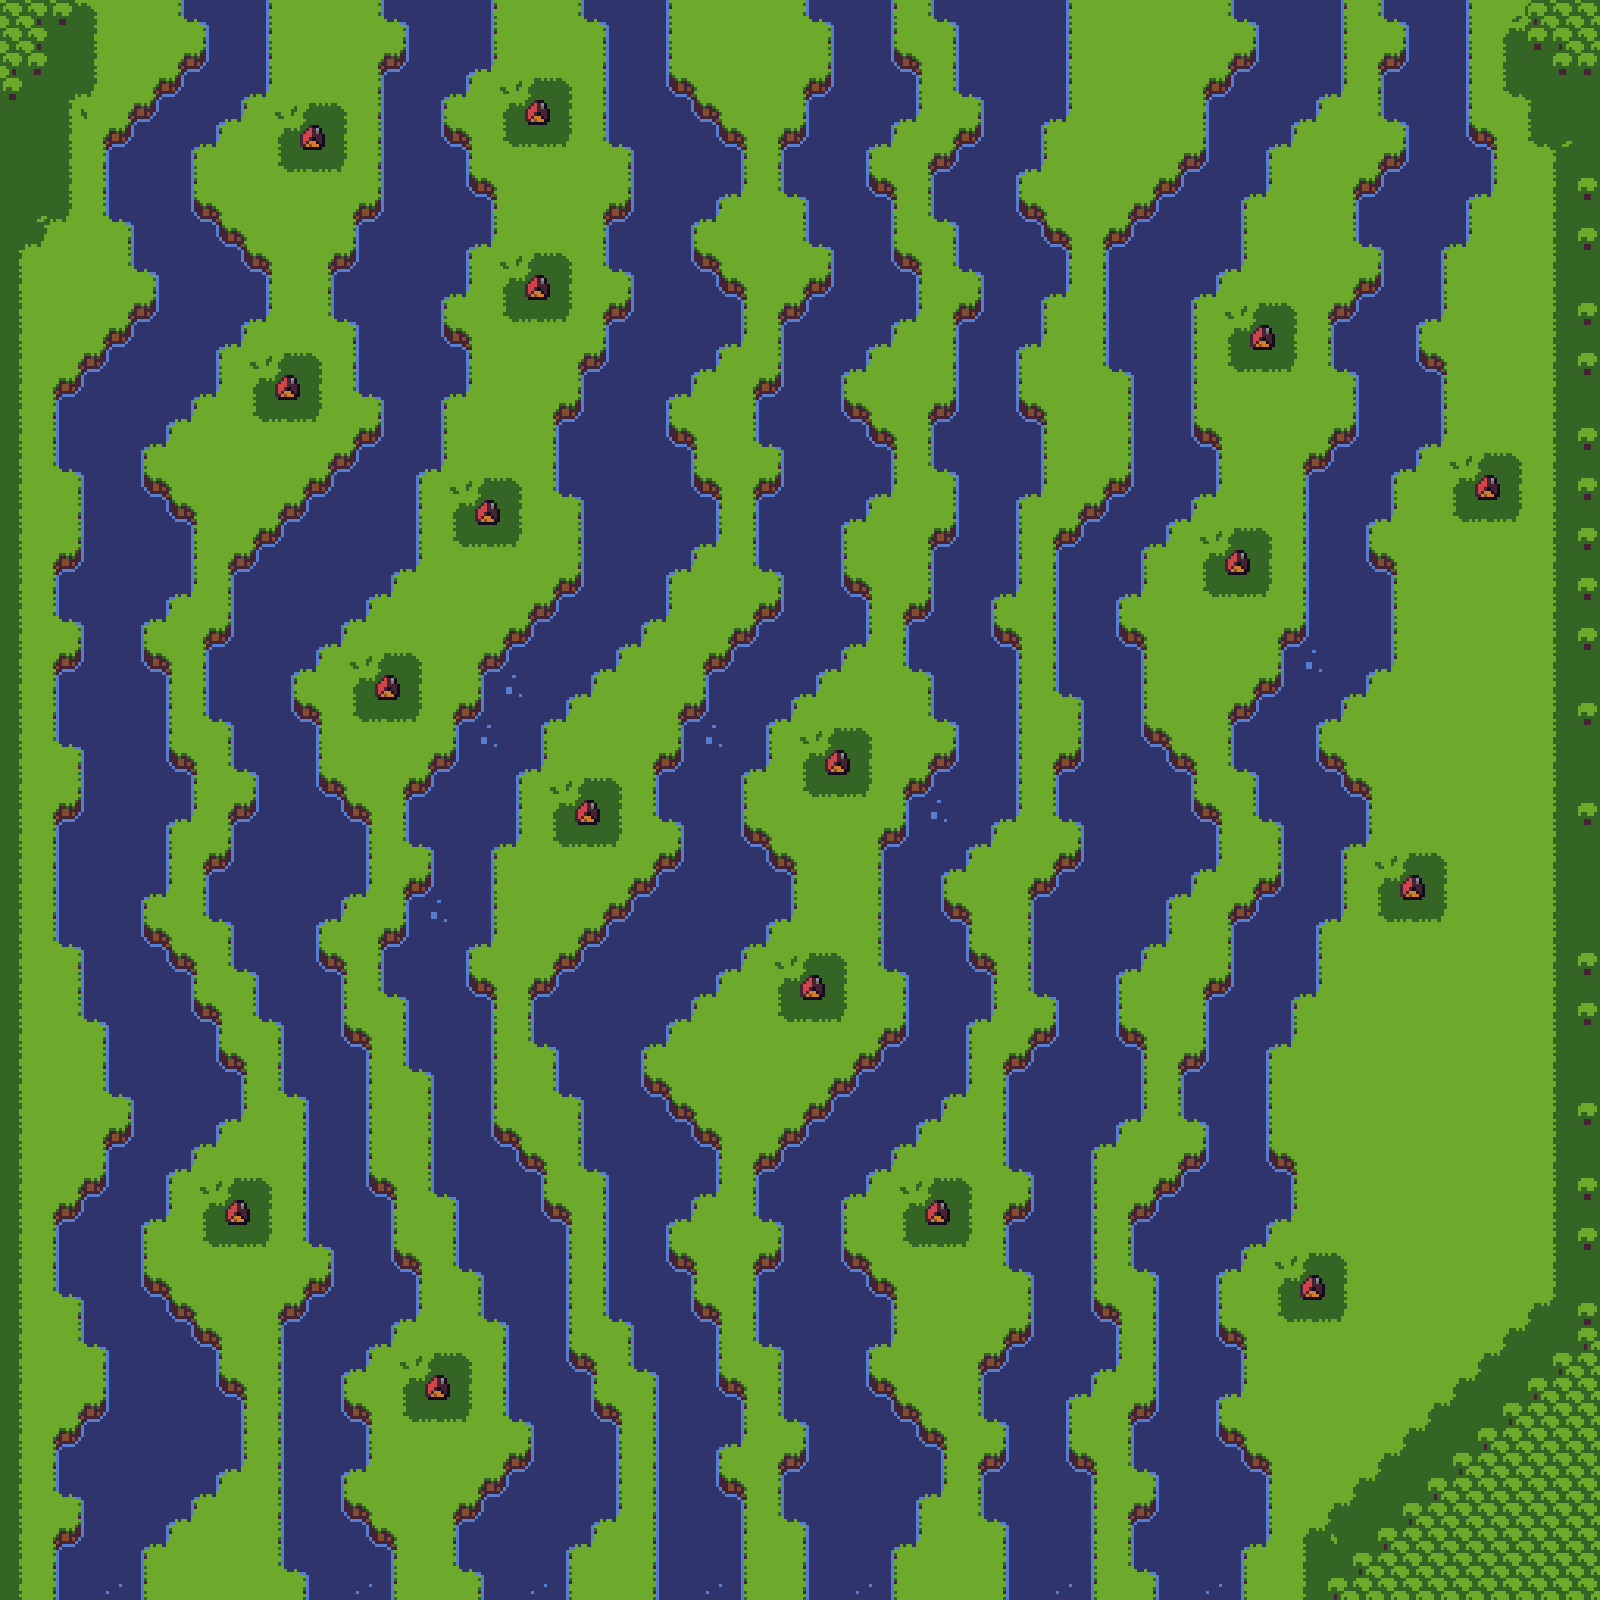
\includegraphics[width=0.9\textwidth]{img/forestmicro_64x64.pdf}
        \end{block}
    \end{columns}
  \end{frame}

  % summary_related_work

  \begin{frame}[fragile]{Related Work}

\begin{table}[h]
  \centering
  \begin{tabular}[t]{l|cccc}
      & \textit{WFC} & \textit{BMS} & \textit{MMS} & \textit{POMS} \\
    \hline
    \specialcellCenter{Solver Type} & Block & Block & Grid & \textbf{Grid} \\
    \specialcellCenter{Contradiction \\ \ \ Resilience} & No & Yes & Yes & \textbf{Yes} \\
    \specialcellCenter{Block Step \ \ \ \ \\ \ \ \ \ Consistent} & n/a & n/a & Yes & \textit{\textbf{No}} \\
    \specialcellCenter{Indeterminate \\ \ \ Initial State} & Yes & Yes & No & \textbf{Yes} \\
    \specialcellCenter{Ergodic} & Yes & Yes & No & \textbf{Yes} \\
    \hline
  \end{tabular}

\end{table}

  \end{frame}

  %%
  %% tile_influence

  \begin{frame}[fragile]{Related Work}
    \begin{columns}[T,onlytextwidth]
      \column{0.5\textwidth}
        \begin{block}{Intuition}
          \hfill \\
          How much influence does a tile choice have over long distances? \\
          \hfill \\
          Difficult to define and/or calculate \\
          \hfill \\
          As a heuristic, \\
          \textit{Tile Arc Consistent Correlation Length} (\textit{TACCL}) 
            from Hoetzlein's \textit{just\_math} project
        \end{block}
      \column{0.5\textwidth}
        \begin{block}{Example}
          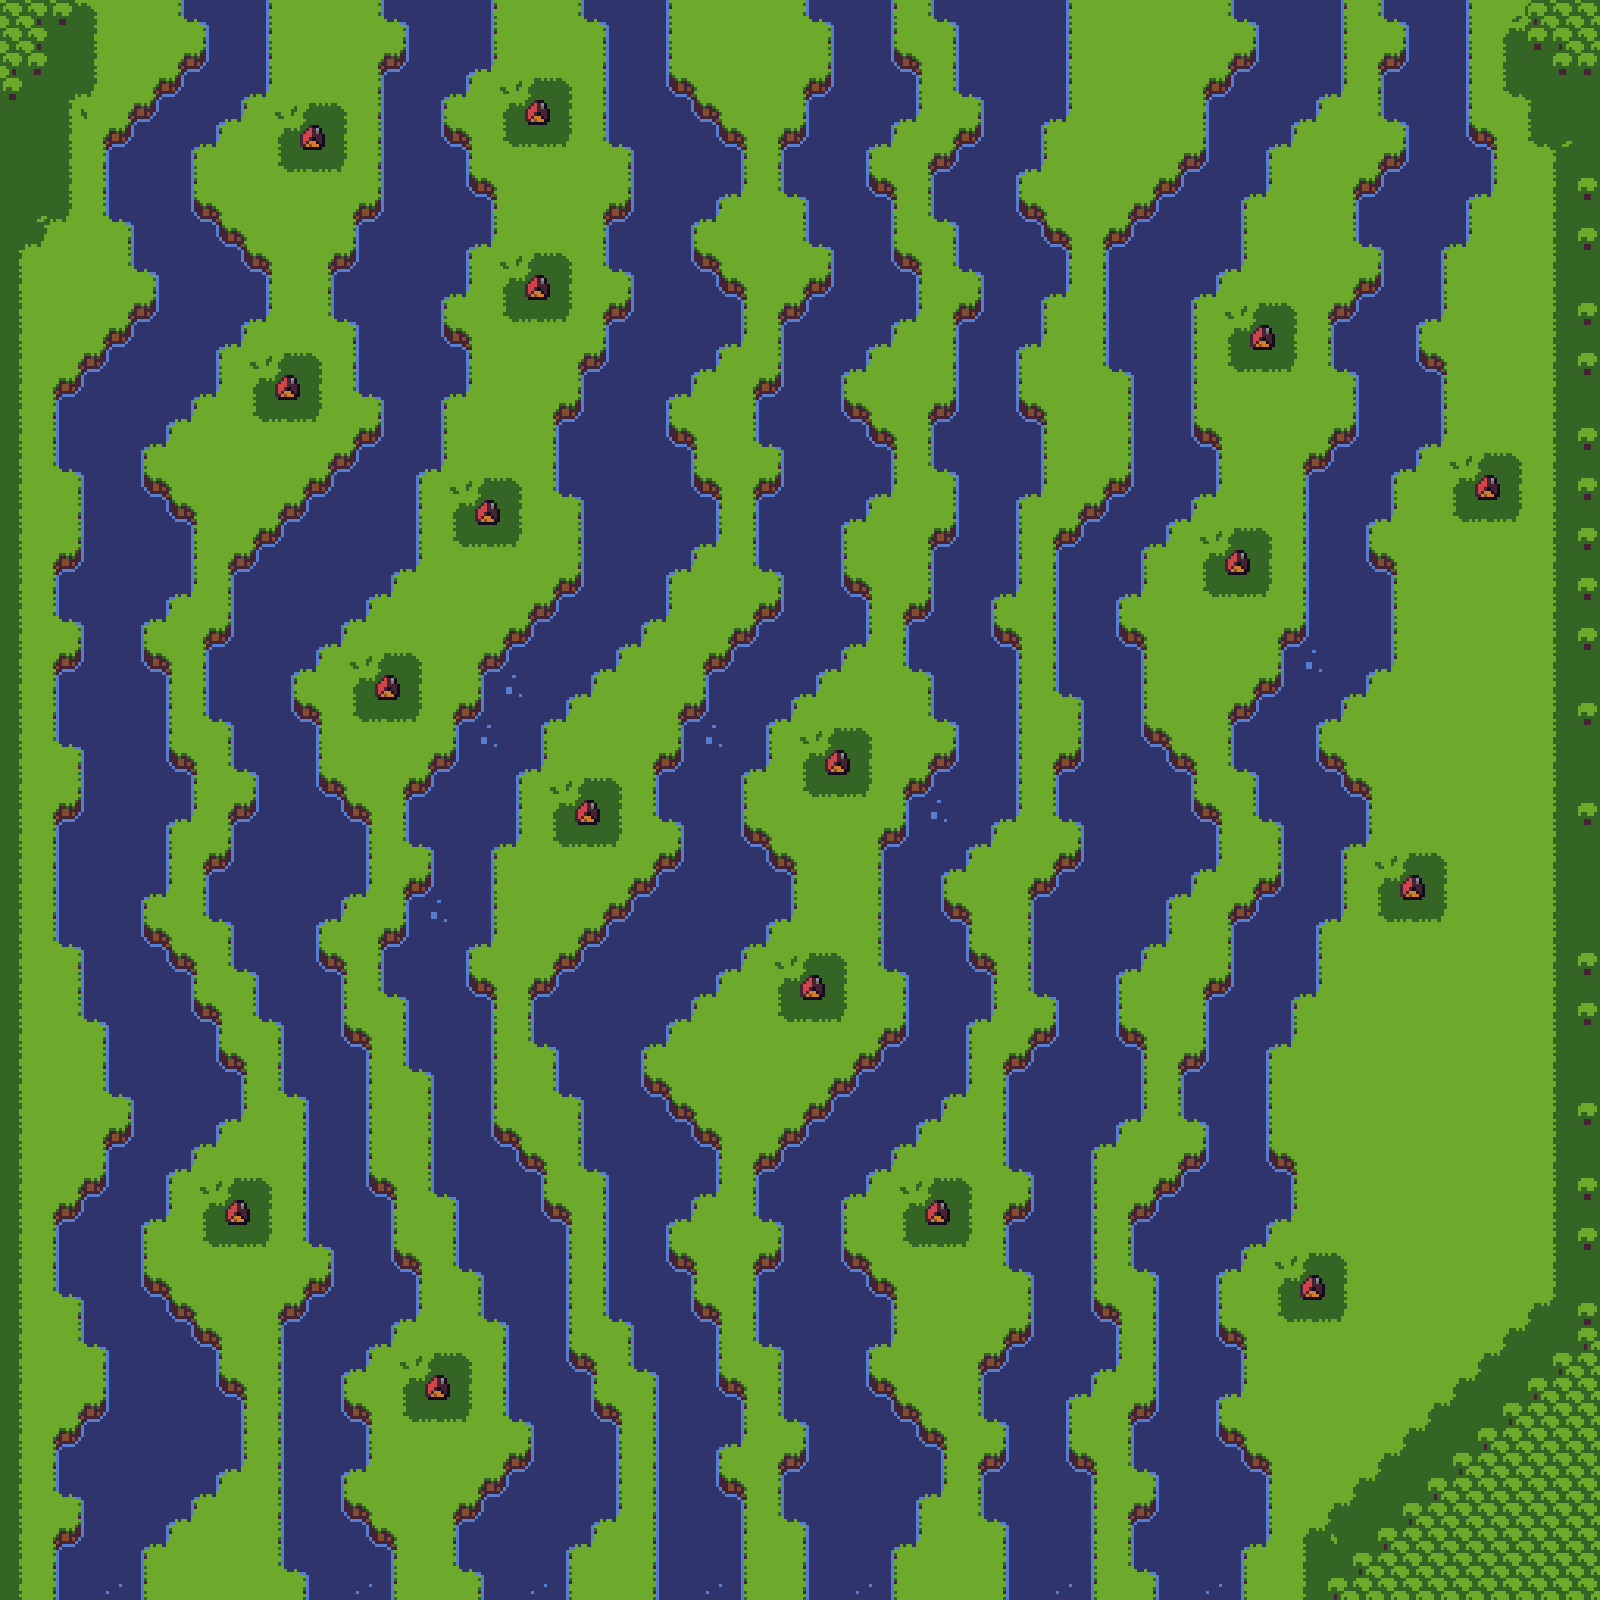
\includegraphics[width=0.9\textwidth]{img/forestmicro_64x64.pdf}
        \end{block}
    \end{columns}
  \end{frame}

  %%

  \begin{frame}[fragile]{Related Work}
    \textit{Tile Arc Consistent Correlation Length} (\textit{TACCL})
    \begin{columns}[T,onlytextwidth]
      \column{0.5\textwidth}
        \begin{block}{TACCL}
          \hfill \\
          \begin{itemize}
            \item Take block in isolation
          \end{itemize}
        \end{block}
      \column{0.5\textwidth}
        \begin{block}{Example}
          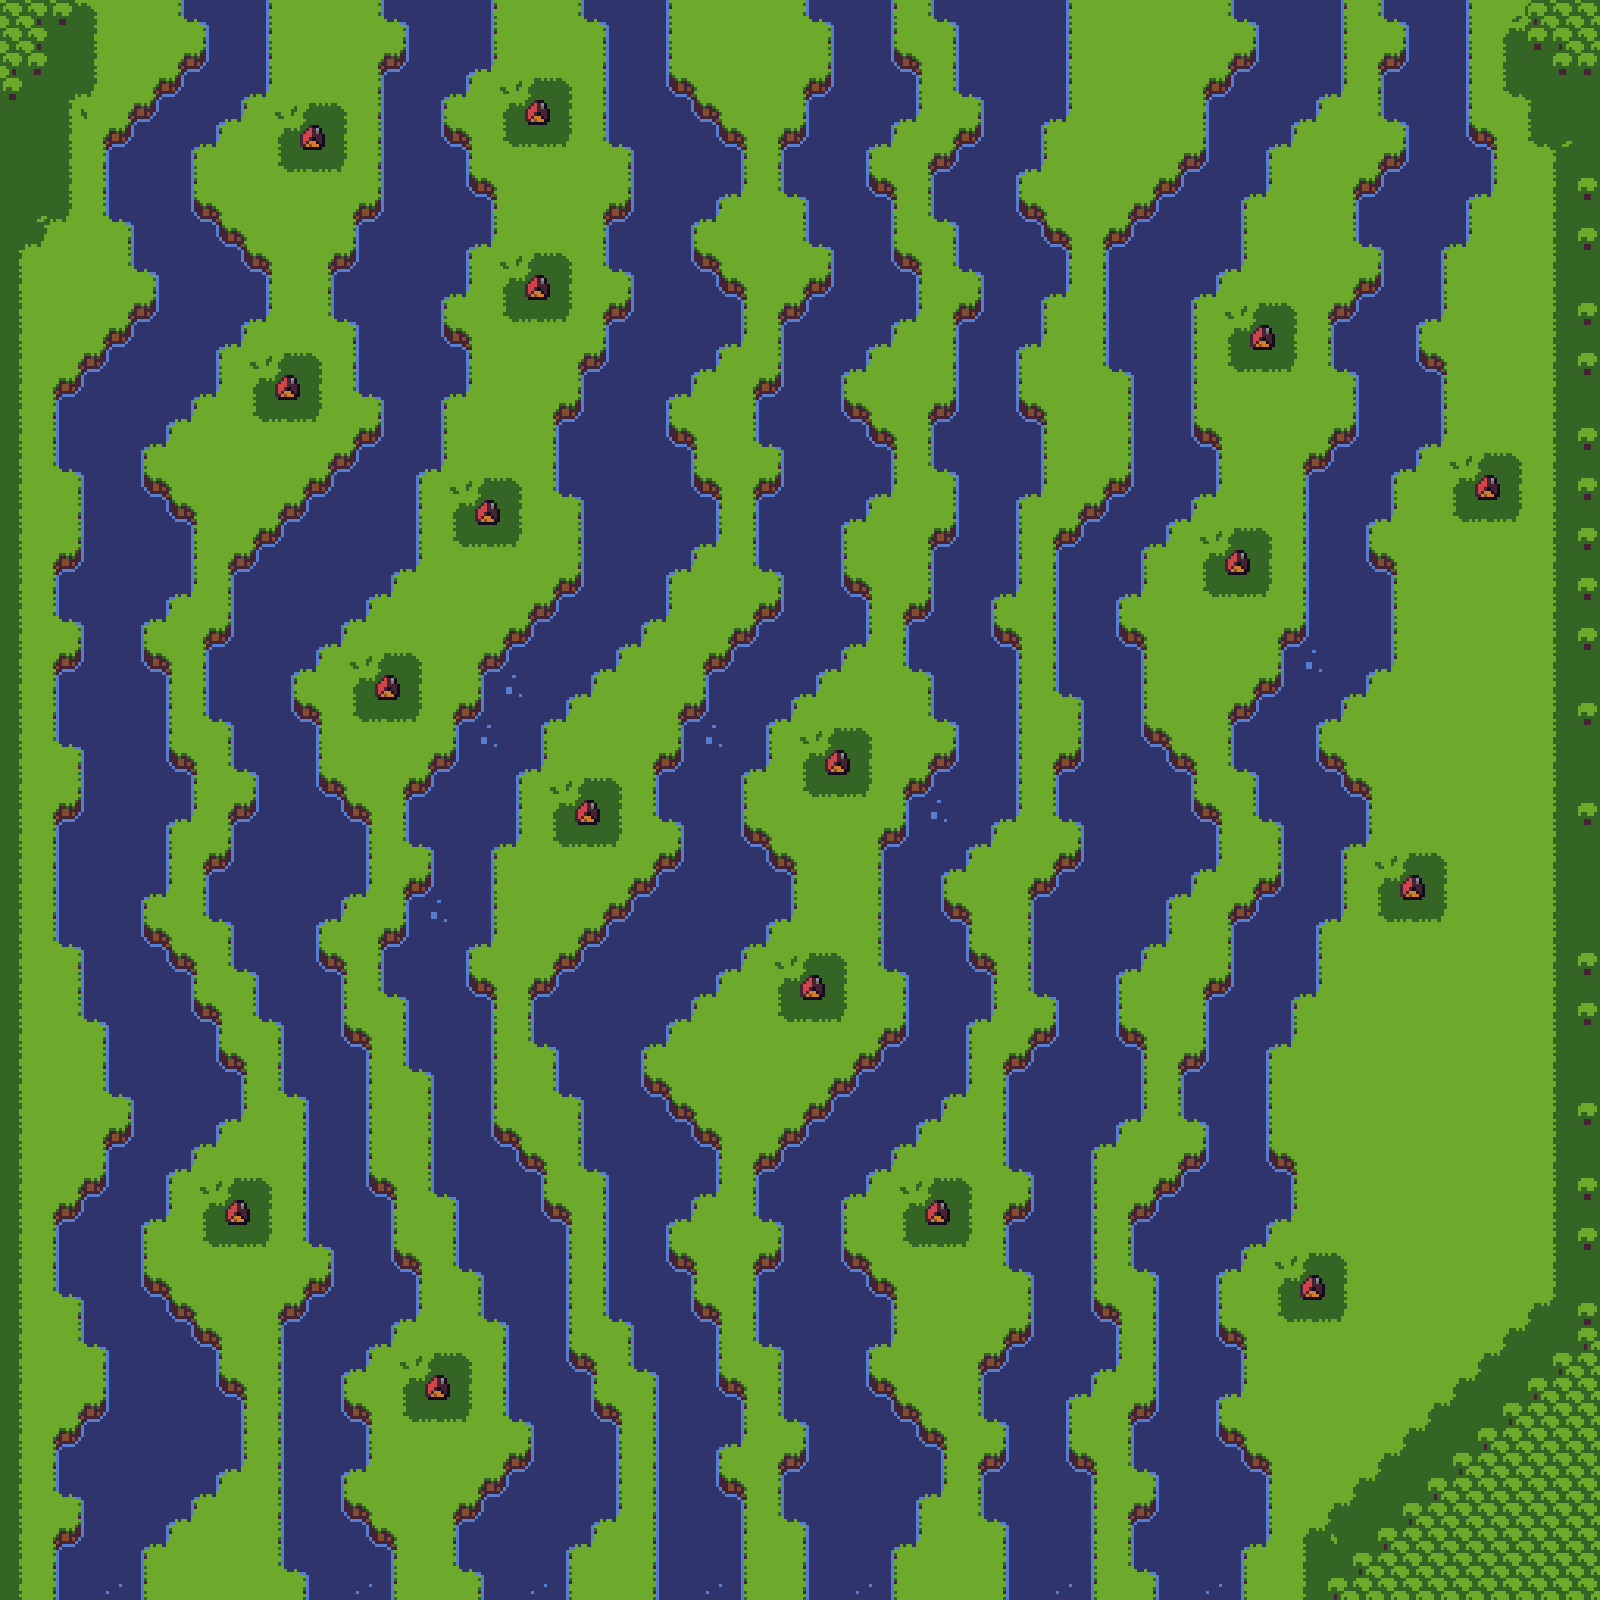
\includegraphics[width=0.9\textwidth]{img/forestmicro_64x64.pdf}
        \end{block}
    \end{columns}
  \end{frame}

  \begin{frame}[fragile]{Related Work}
    \textit{Tile Arc Consistent Correlation Length} (\textit{TACCL})
    \begin{columns}[T,onlytextwidth]
      \column{0.5\textwidth}
        \begin{block}{TACCL}
          \hfill \\
          \begin{itemize}
            \item Take block in isolation
            \item Set block to indeterminate state
          \end{itemize}
        \end{block}
      \column{0.5\textwidth}
        \begin{block}{Example}
          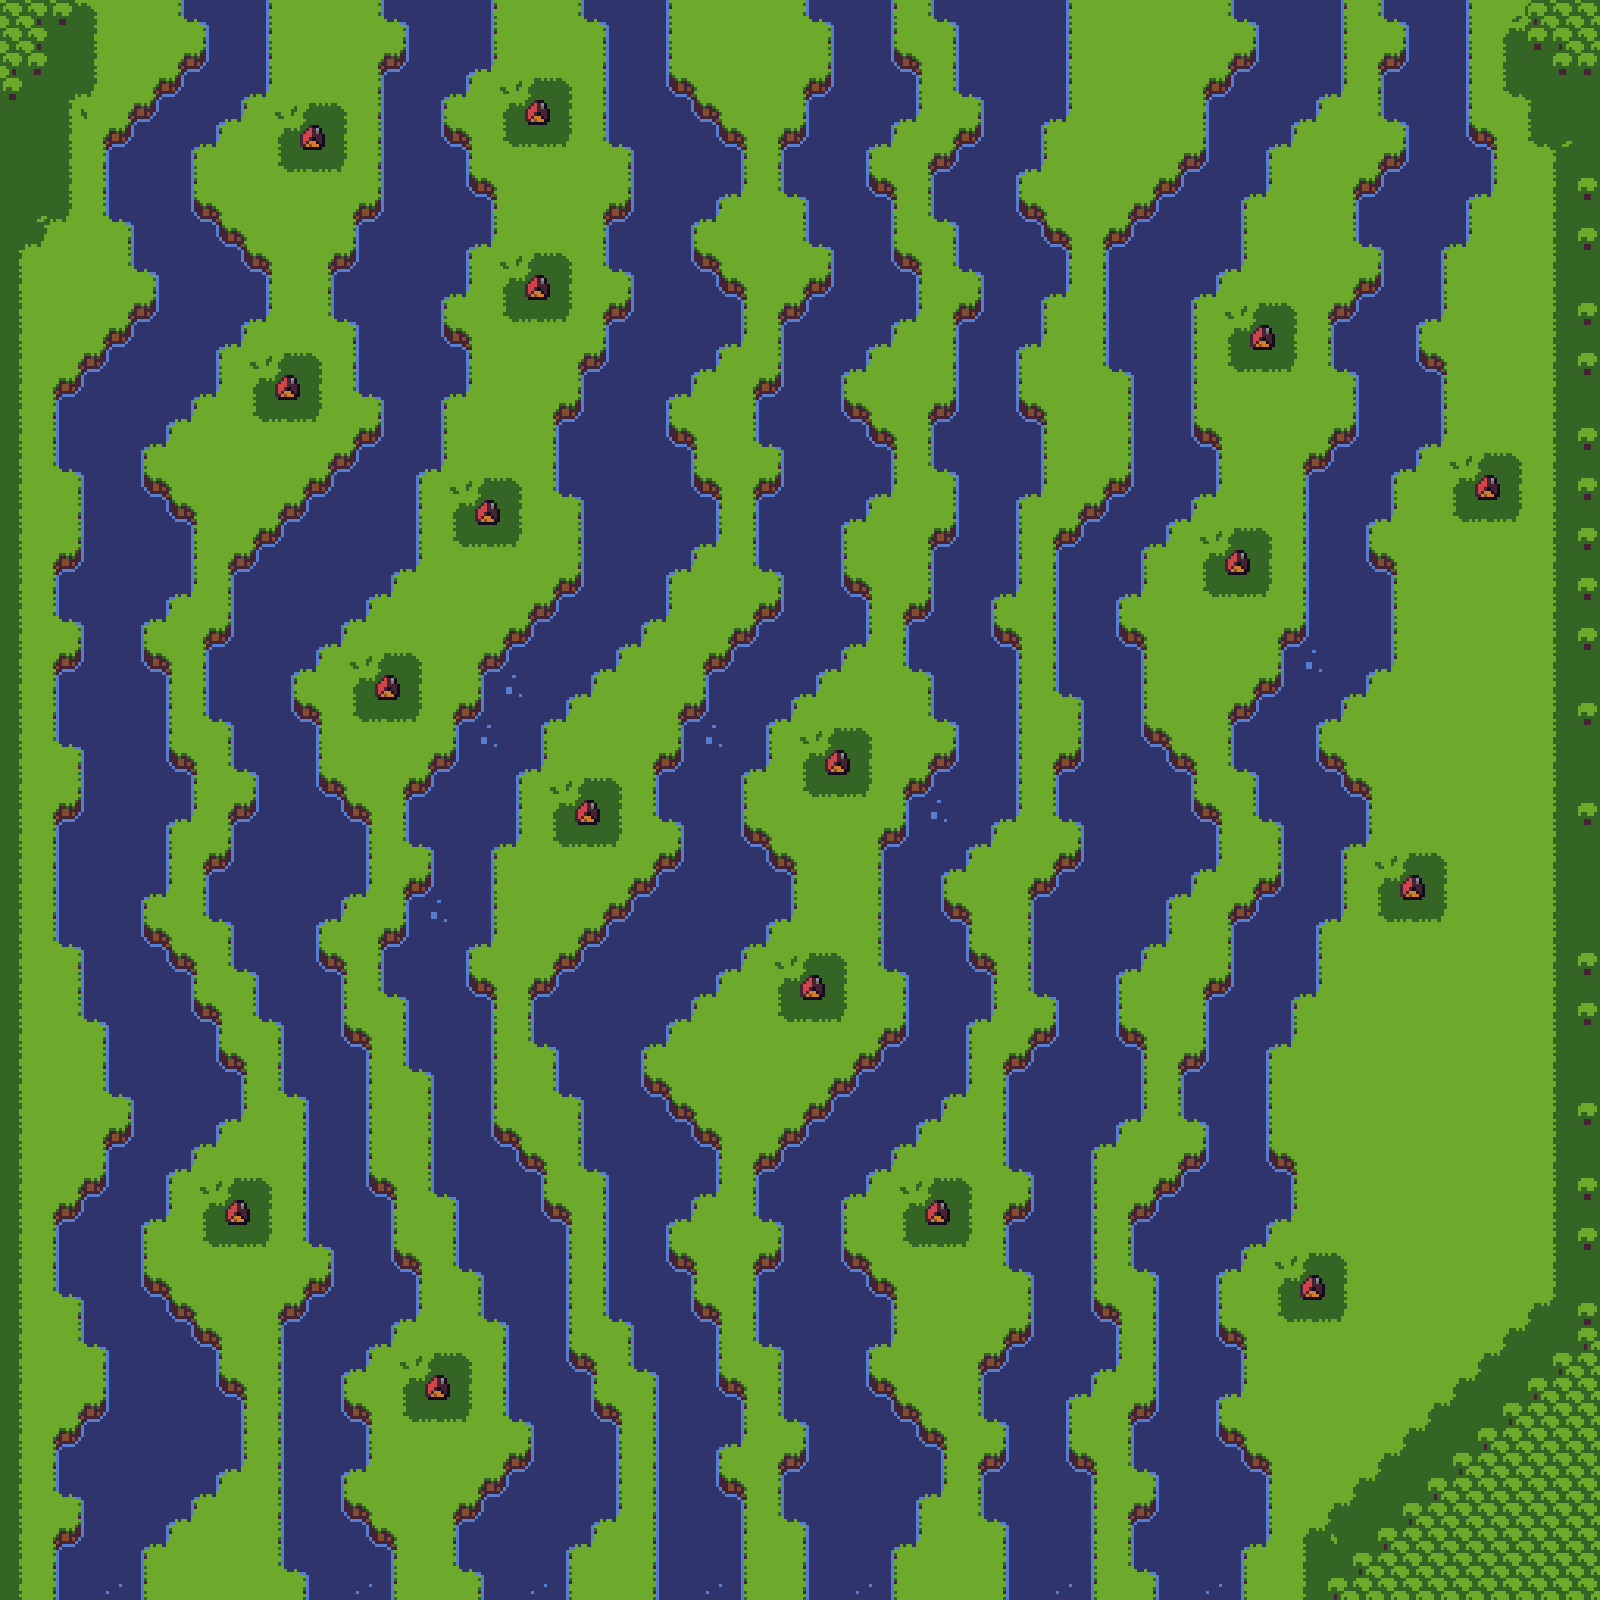
\includegraphics[width=0.9\textwidth]{img/forestmicro_64x64.pdf}
        \end{block}
    \end{columns}
  \end{frame}

  \begin{frame}[fragile]{Related Work}
    \textit{Tile Arc Consistent Correlation Length} (\textit{TACCL})
    \begin{columns}[T,onlytextwidth]
      \column{0.5\textwidth}
        \begin{block}{TACCL}
          \hfill \\
          \begin{itemize}
            \item Take block in isolation
            \item Set block to indeterminate state
            \item Fix a tile at the center
          \end{itemize}
        \end{block}
      \column{0.5\textwidth}
        \begin{block}{Example}
          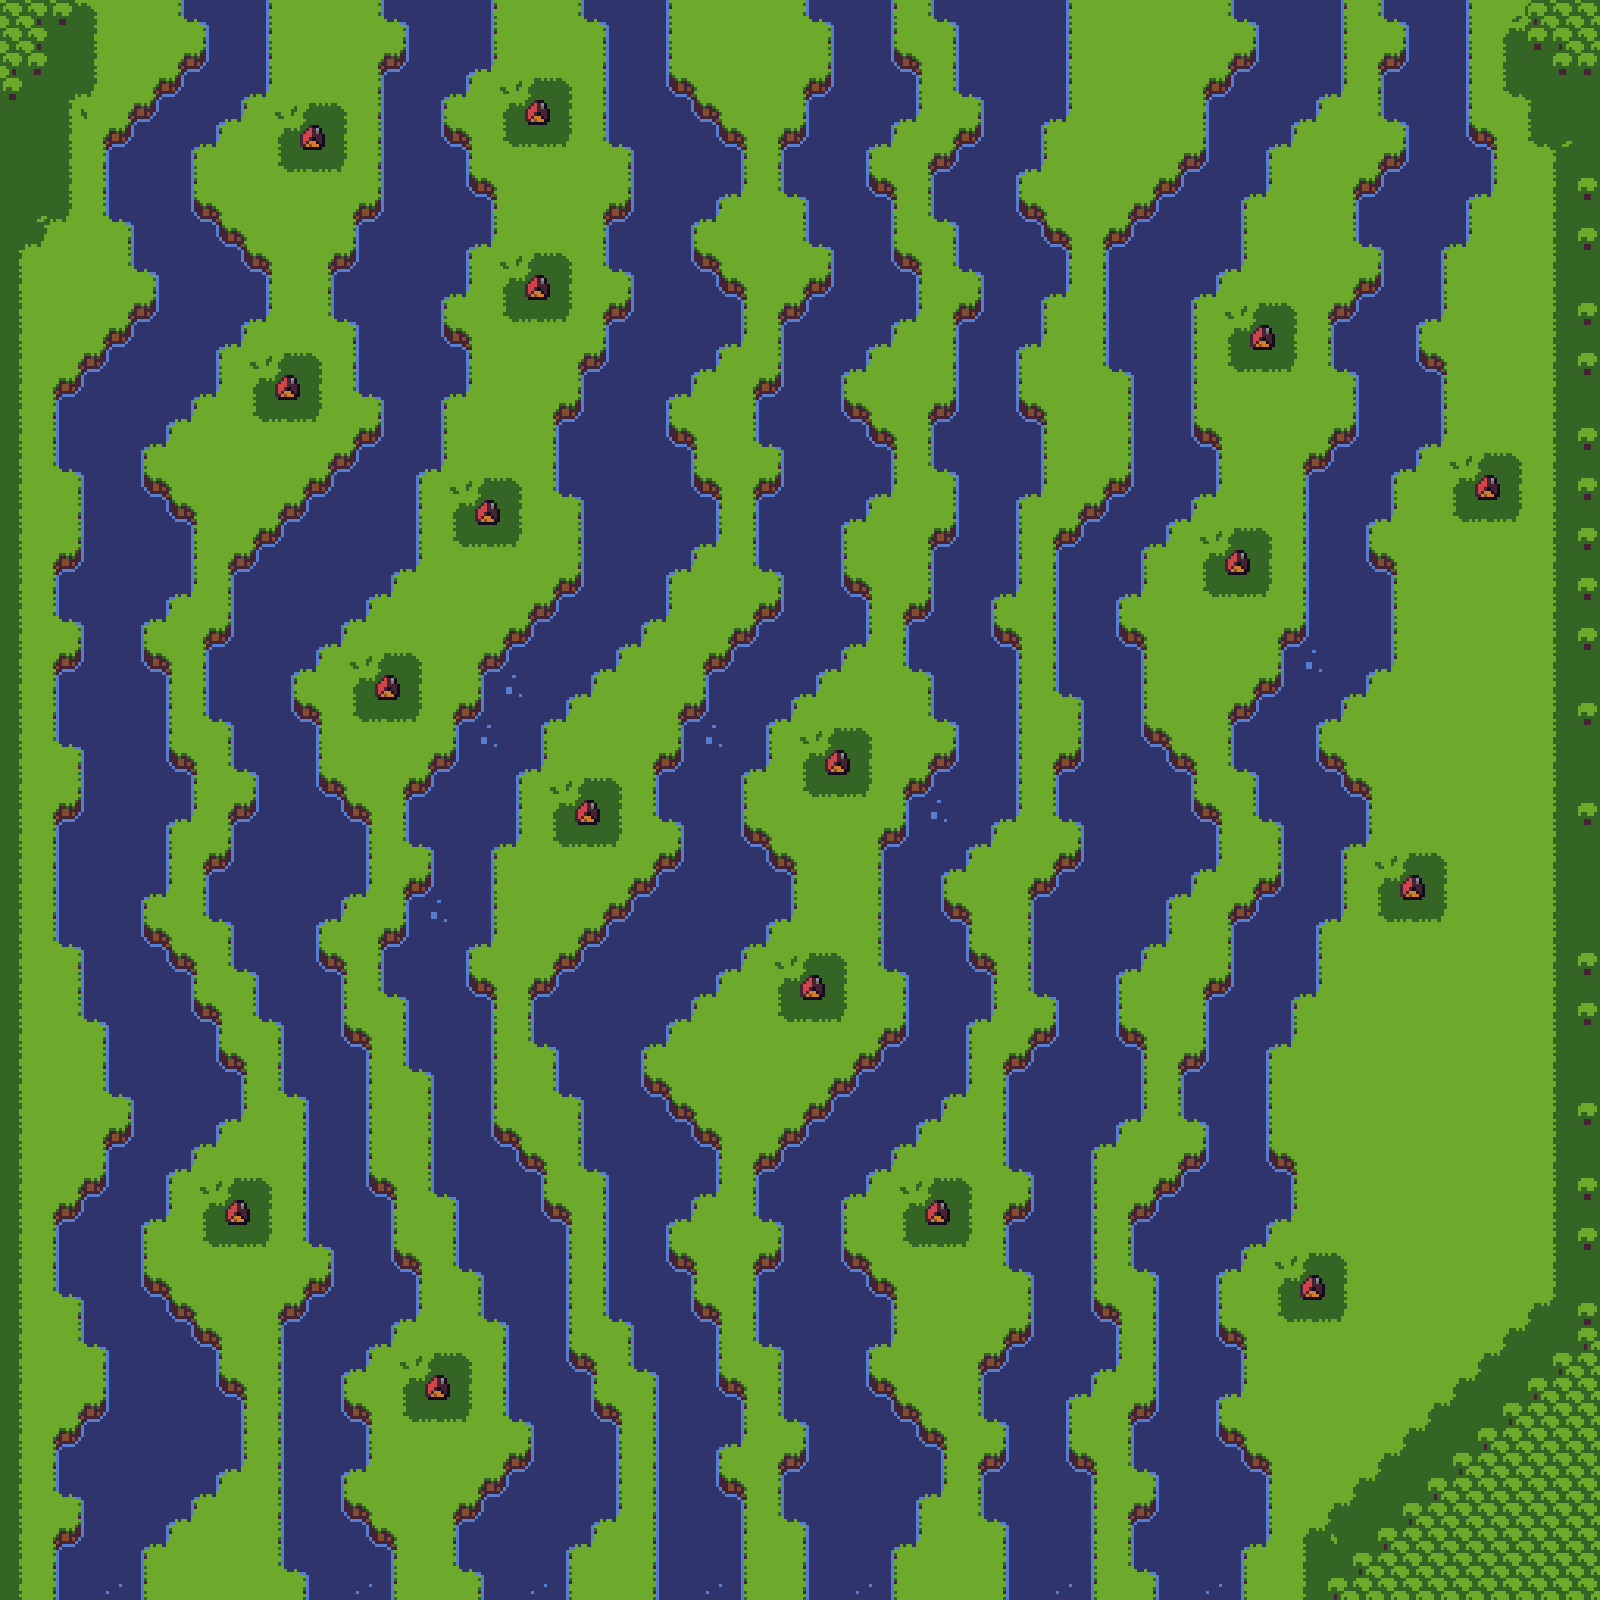
\includegraphics[width=0.9\textwidth]{img/forestmicro_64x64.pdf}
        \end{block}
    \end{columns}
  \end{frame}

  \begin{frame}[fragile]{Related Work}
    \textit{Tile Arc Consistent Correlation Length} (\textit{TACCL})
    \begin{columns}[T,onlytextwidth]
      \column{0.5\textwidth}
        \begin{block}{TACCL}
          \hfill \\
          \begin{itemize}
            \item Take block in isolation
            \item Set block to indeterminate state
            \item Fix a tile at the center
            \item Propagate constraints
          \end{itemize}
        \end{block}
      \column{0.5\textwidth}
        \begin{block}{Example}
          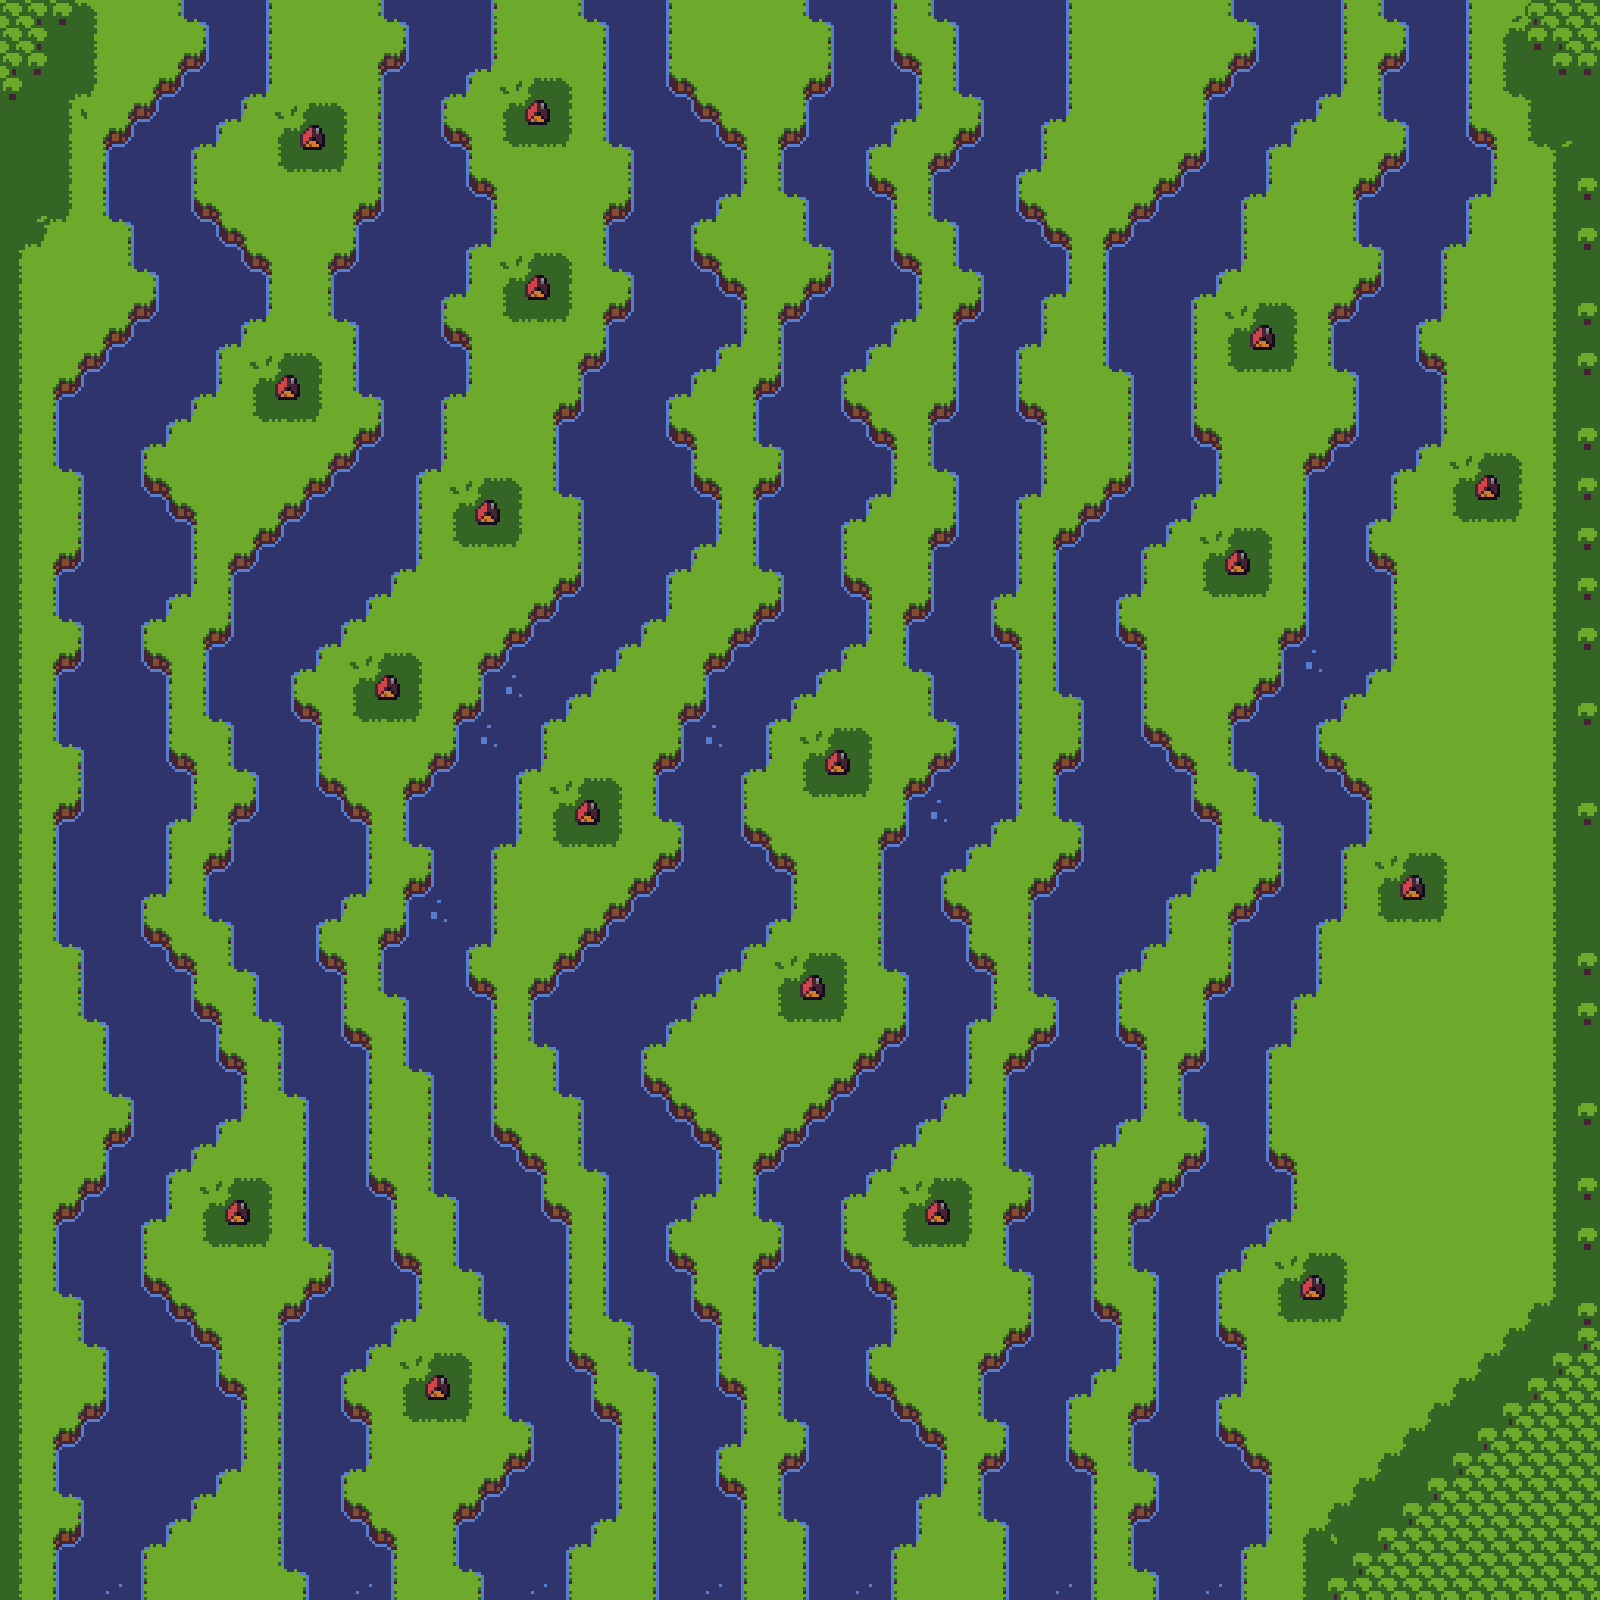
\includegraphics[width=0.9\textwidth]{img/forestmicro_64x64.pdf}
        \end{block}
    \end{columns}
  \end{frame}

  \begin{frame}[fragile]{Related Work}
    \textit{Tile Arc Consistent Correlation Length} (\textit{TACCL})
    \begin{columns}[T,onlytextwidth]
      \column{0.5\textwidth}
        \begin{block}{TACCL}
          \hfill \\
          \begin{itemize}
            \item Take block in isolation
            \item Set block to indeterminate state
            \item Fix a tile at the center
            \item Propagate constraints
            \item Take minimum bounding box of altered cells
          \end{itemize}
        \end{block}
      \column{0.5\textwidth}
        \begin{block}{Example}
          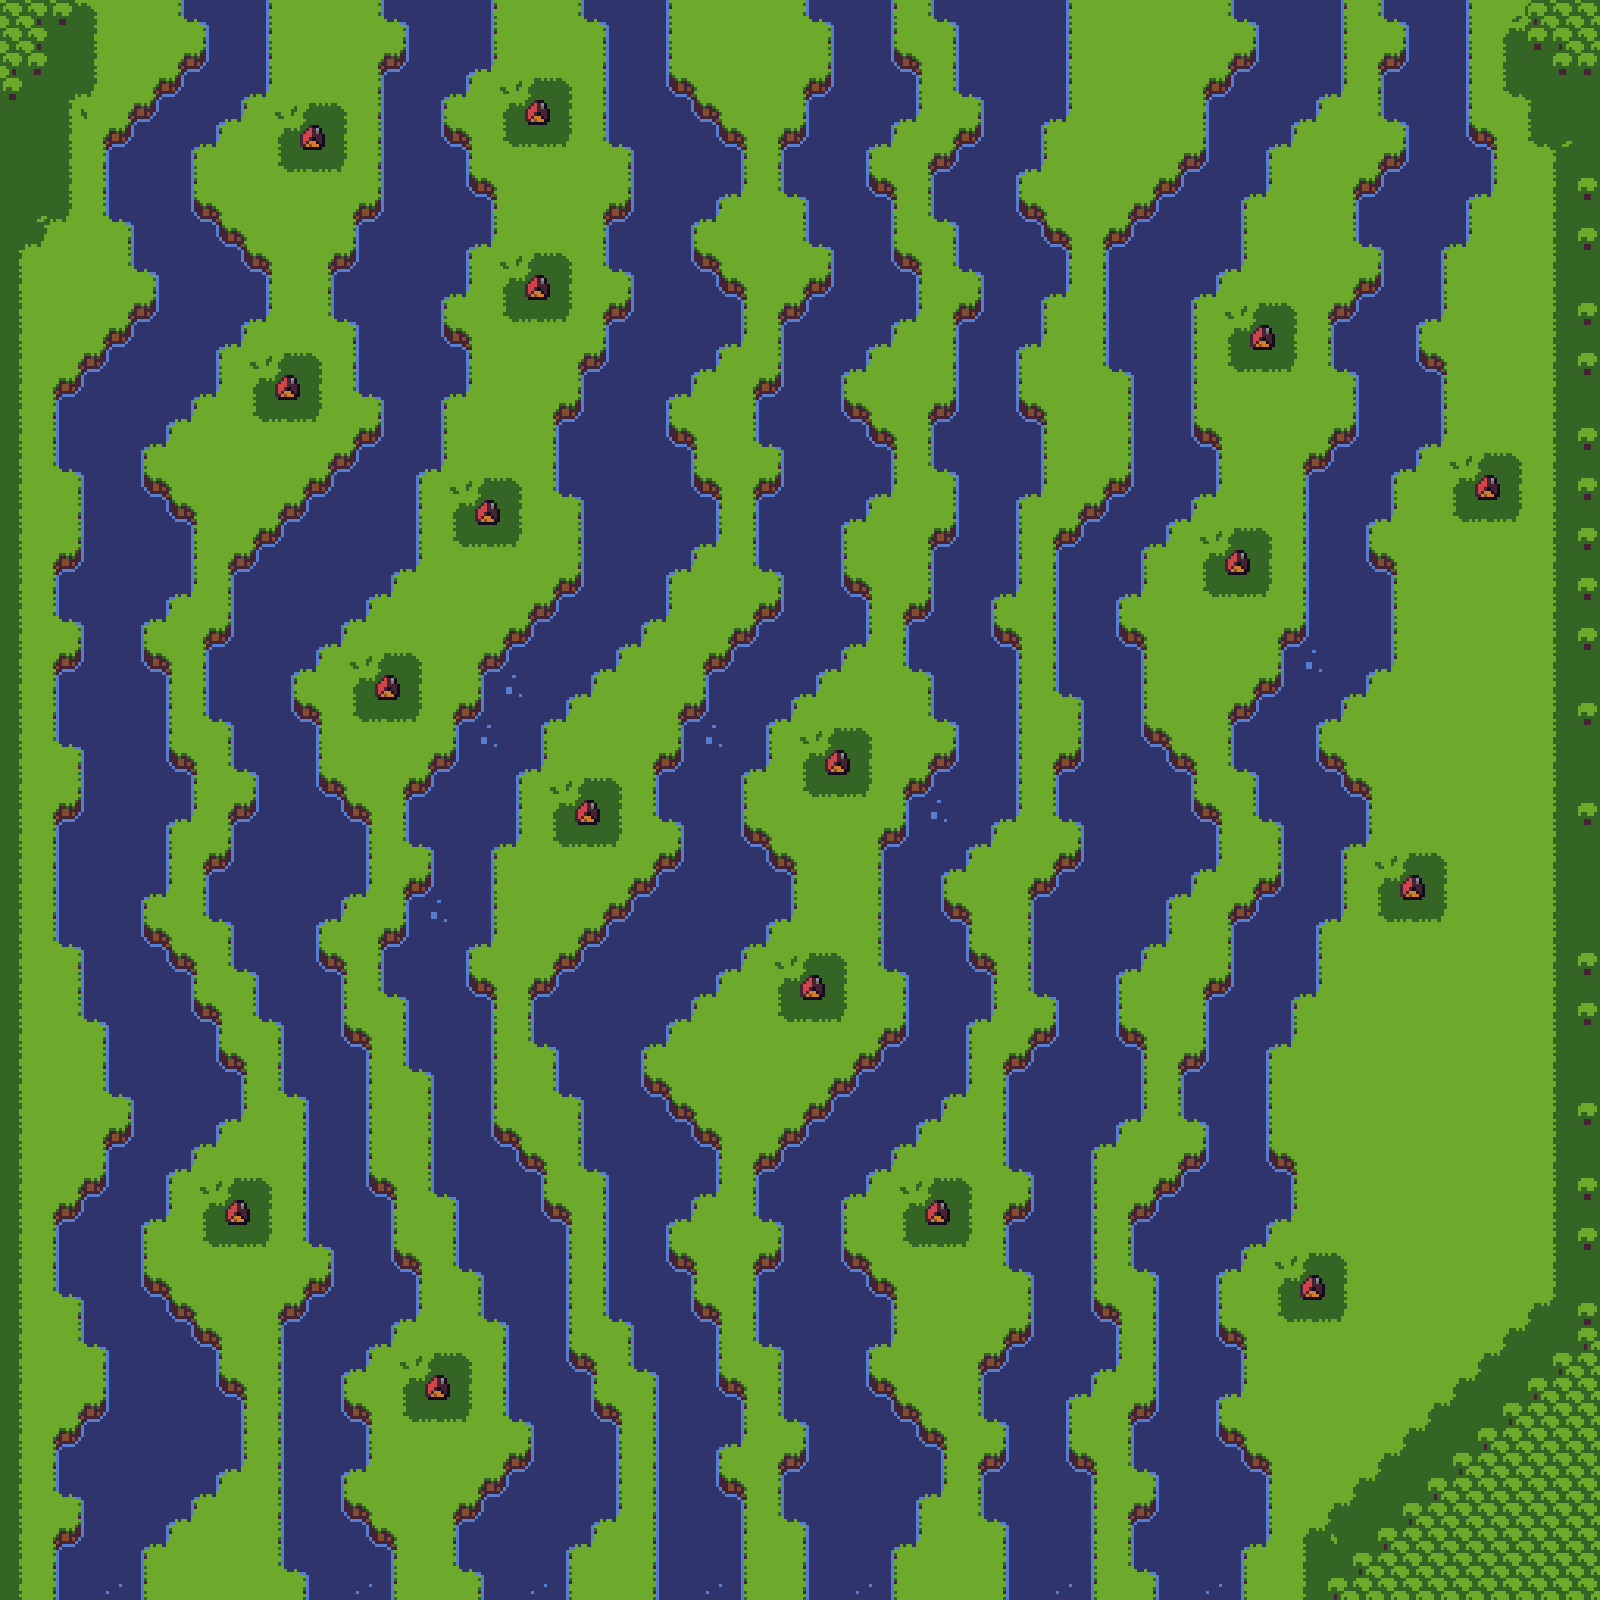
\includegraphics[width=0.9\textwidth]{img/forestmicro_64x64.pdf}
        \end{block}
    \end{columns}
  \end{frame}

  \begin{frame}[fragile]{Related Work}
    \textit{Tile Arc Consistent Correlation Length} (\textit{TACCL})
    \begin{columns}[T,onlytextwidth]
      \column{0.5\textwidth}
        \begin{block}{TACCL}
          \hfill \\
          \begin{itemize}
            \item Take block in isolation
            \item Set block to indeterminate state
            \item Fix a tile at the center
            \item Propagate constraints
            \item Take minimum bounding box of altered cells
            \item Repeat for all tiles
          \end{itemize}
        \end{block}
      \column{0.5\textwidth}
        \begin{block}{Example}
          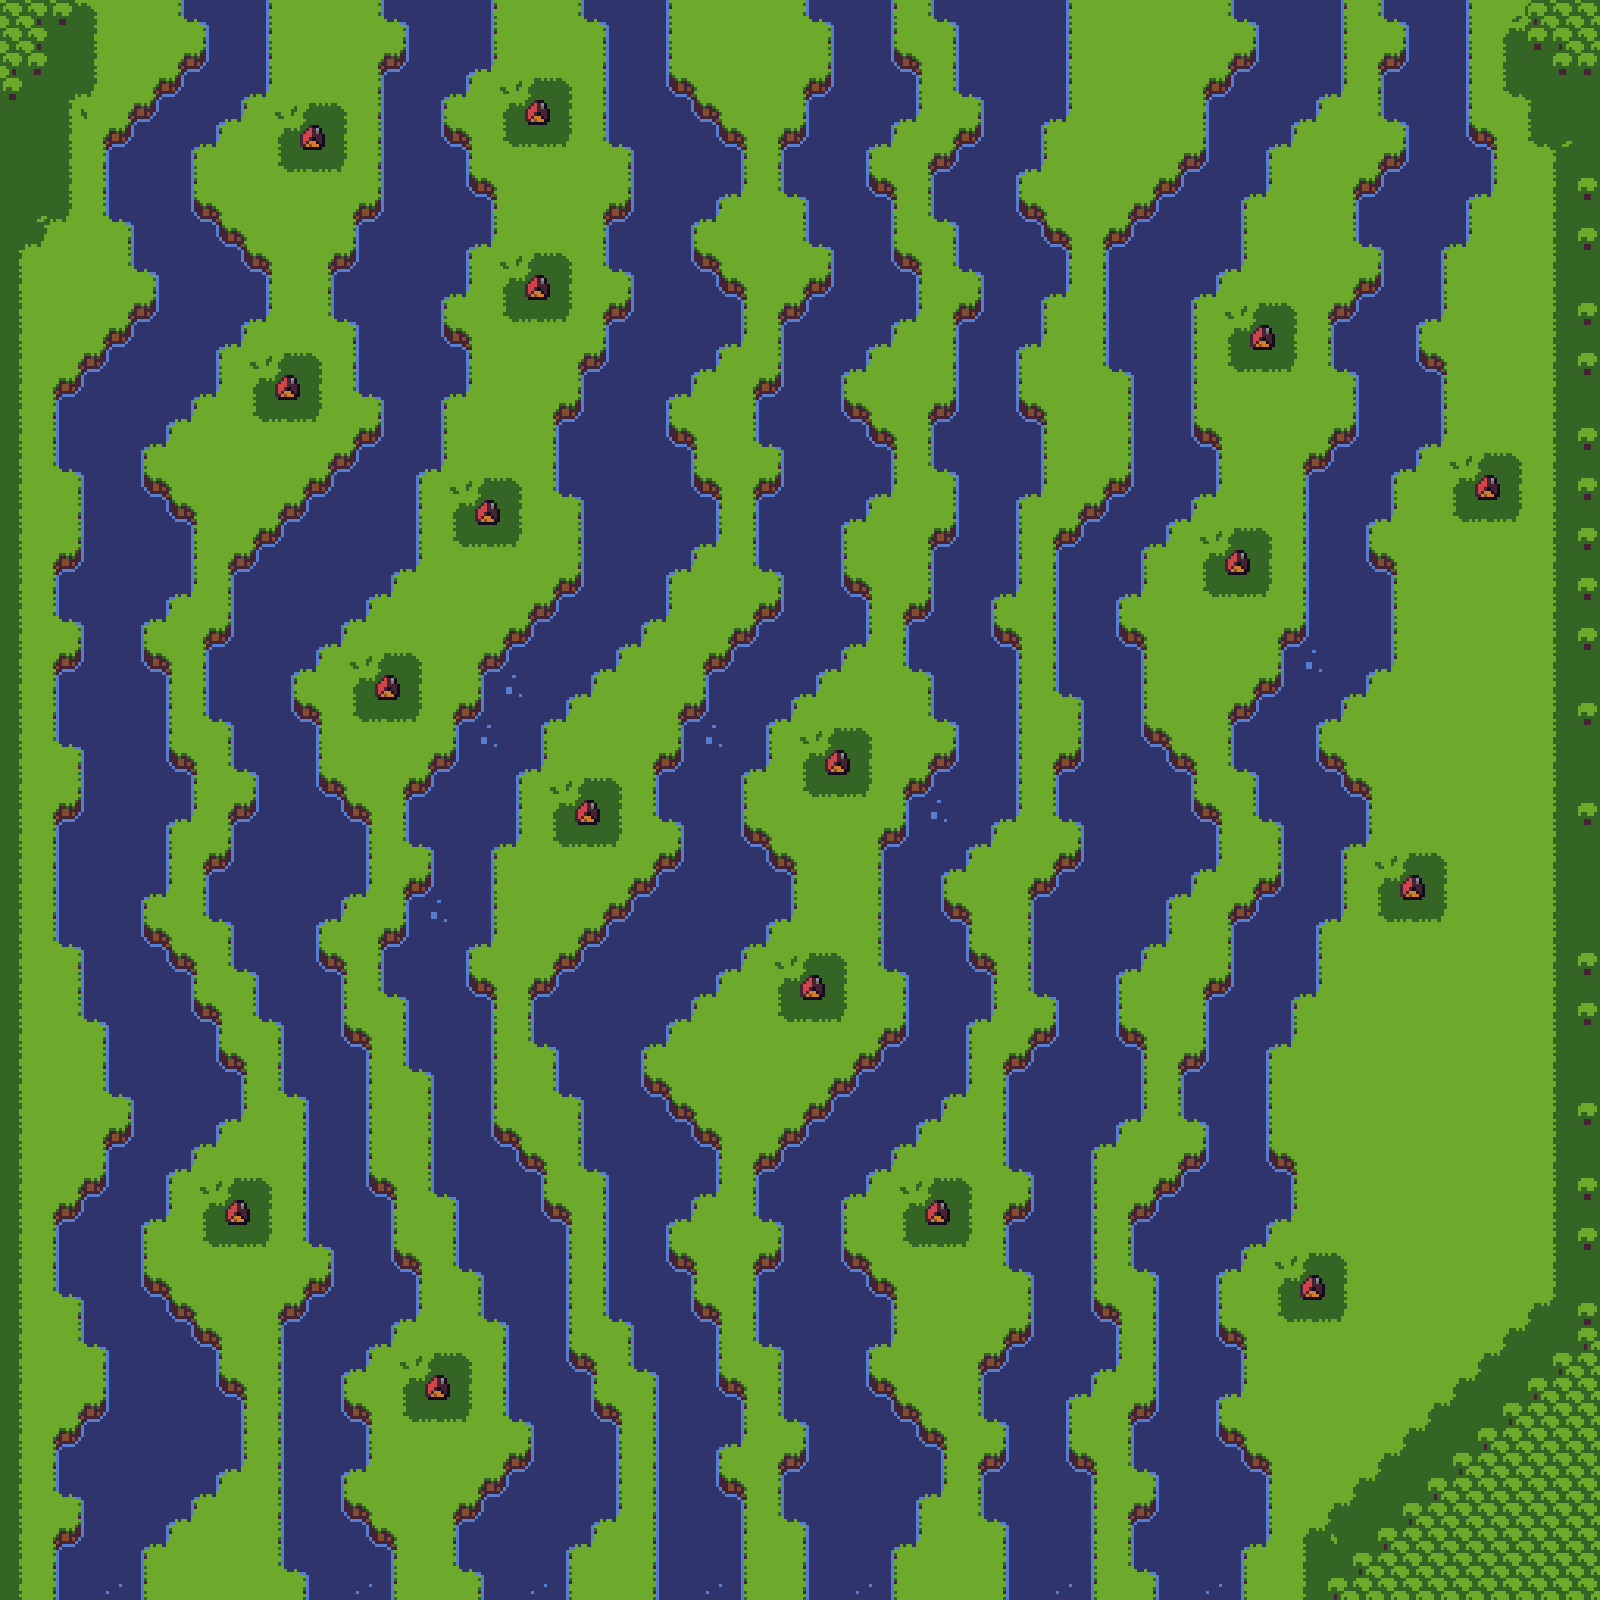
\includegraphics[width=0.9\textwidth]{img/forestmicro_64x64.pdf}
        \end{block}
    \end{columns}
  \end{frame}



  %%%%%%%%%%%%%%%
  %%%%%%%%%%%%%%%
  %%%%%%%%%%%%%%%
  %%%%%%%%%%%%%%%

  %\section{Algorithm}

  \begin{frame}[fragile]{Algorithm: Overview }
    \begin{figure}
      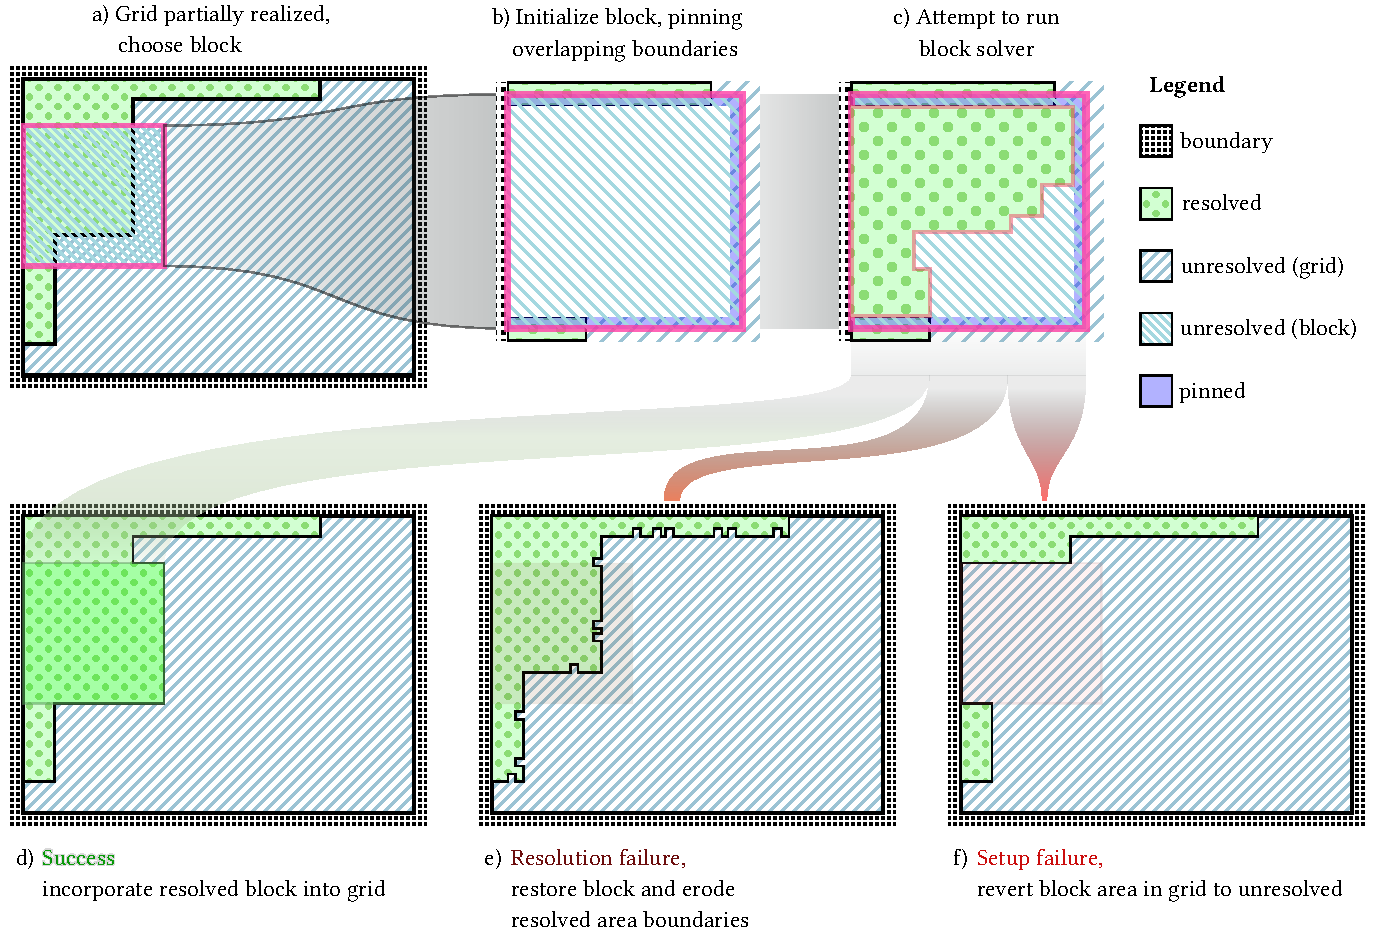
\includegraphics[width=\textwidth]{figs/poms_figalg.pdf}
    \end{figure}
  \end{frame}

  \begin{frame}[fragile]{Algorithm}
    \begin{figure}
      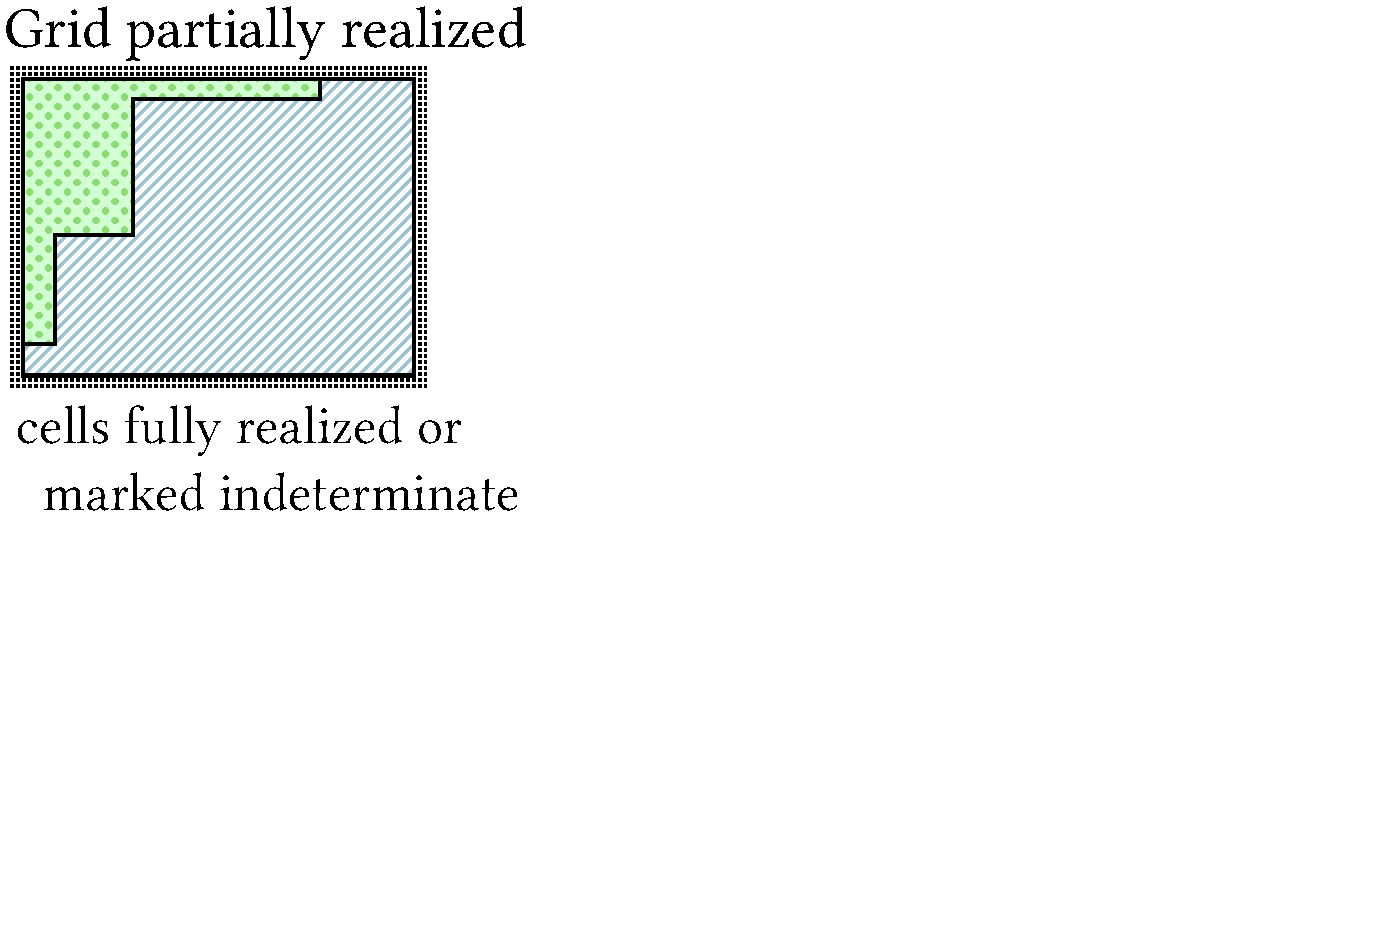
\includegraphics[width=\textwidth]{figs/poms_alg0.pdf}
    \end{figure}
  \end{frame}

  \begin{frame}[fragile]{Algorithm}
    \begin{figure}
      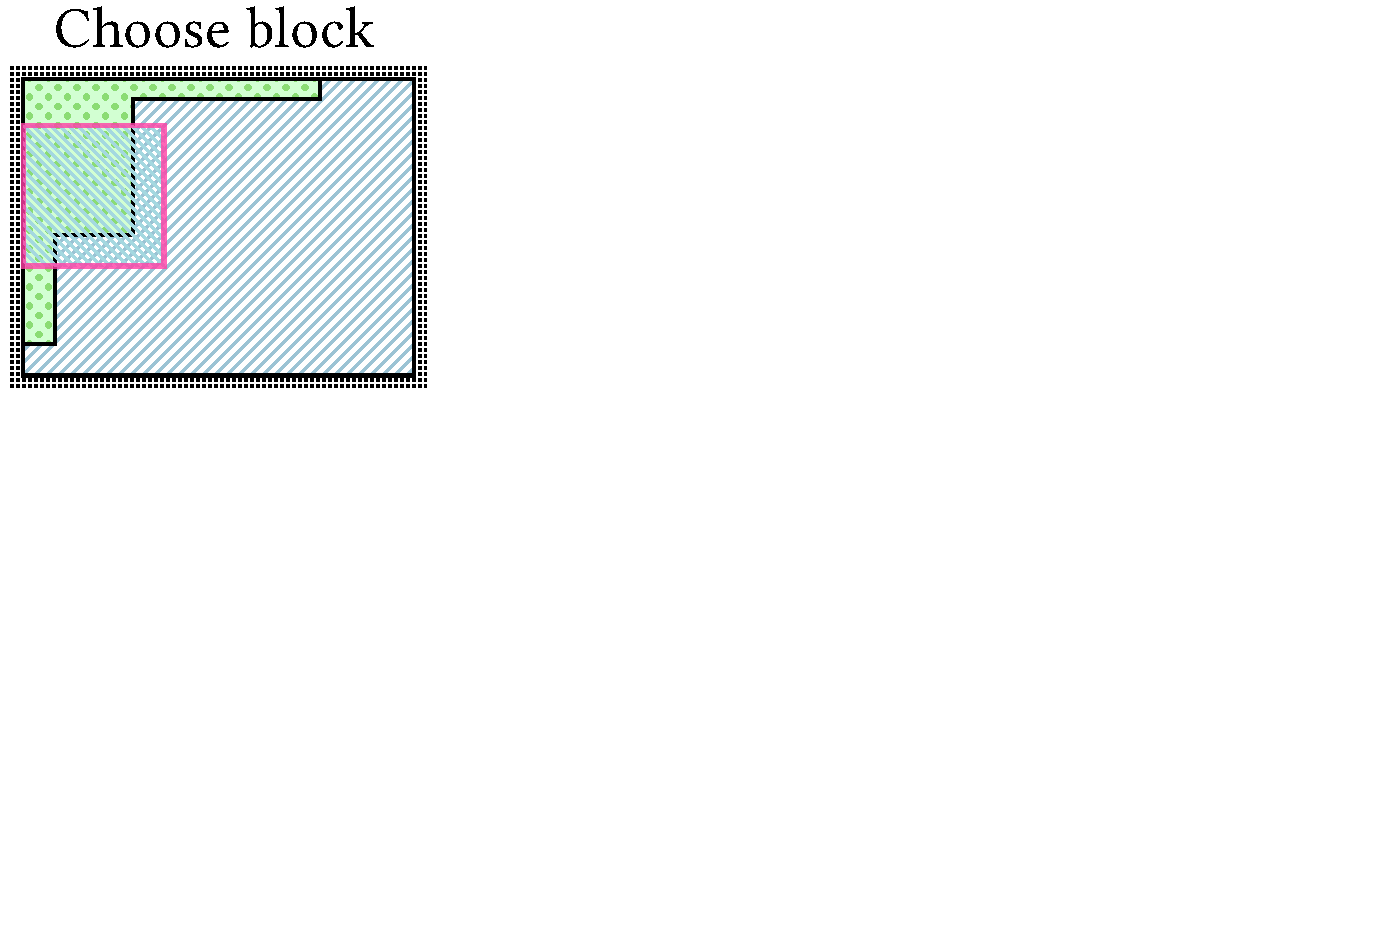
\includegraphics[width=\textwidth]{figs/poms_alg1.pdf}
    \end{figure}
  \end{frame}

  \begin{frame}[fragile]{Algorithm}
    \begin{figure}
      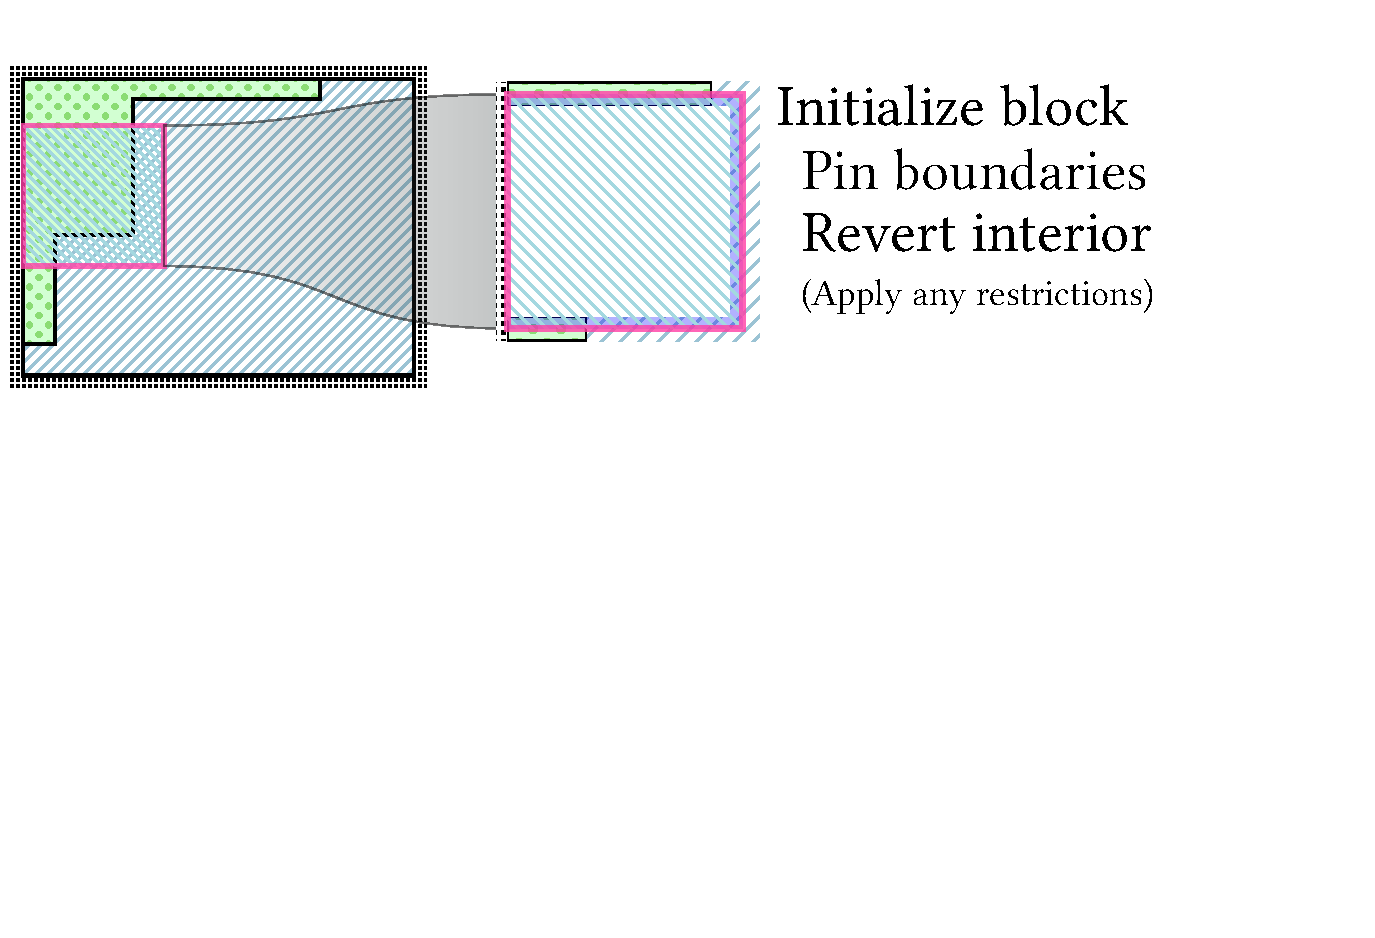
\includegraphics[width=\textwidth]{figs/poms_alg2.pdf}
    \end{figure}
  \end{frame}

  \begin{frame}[fragile]{Algorithm}
    \begin{figure}
      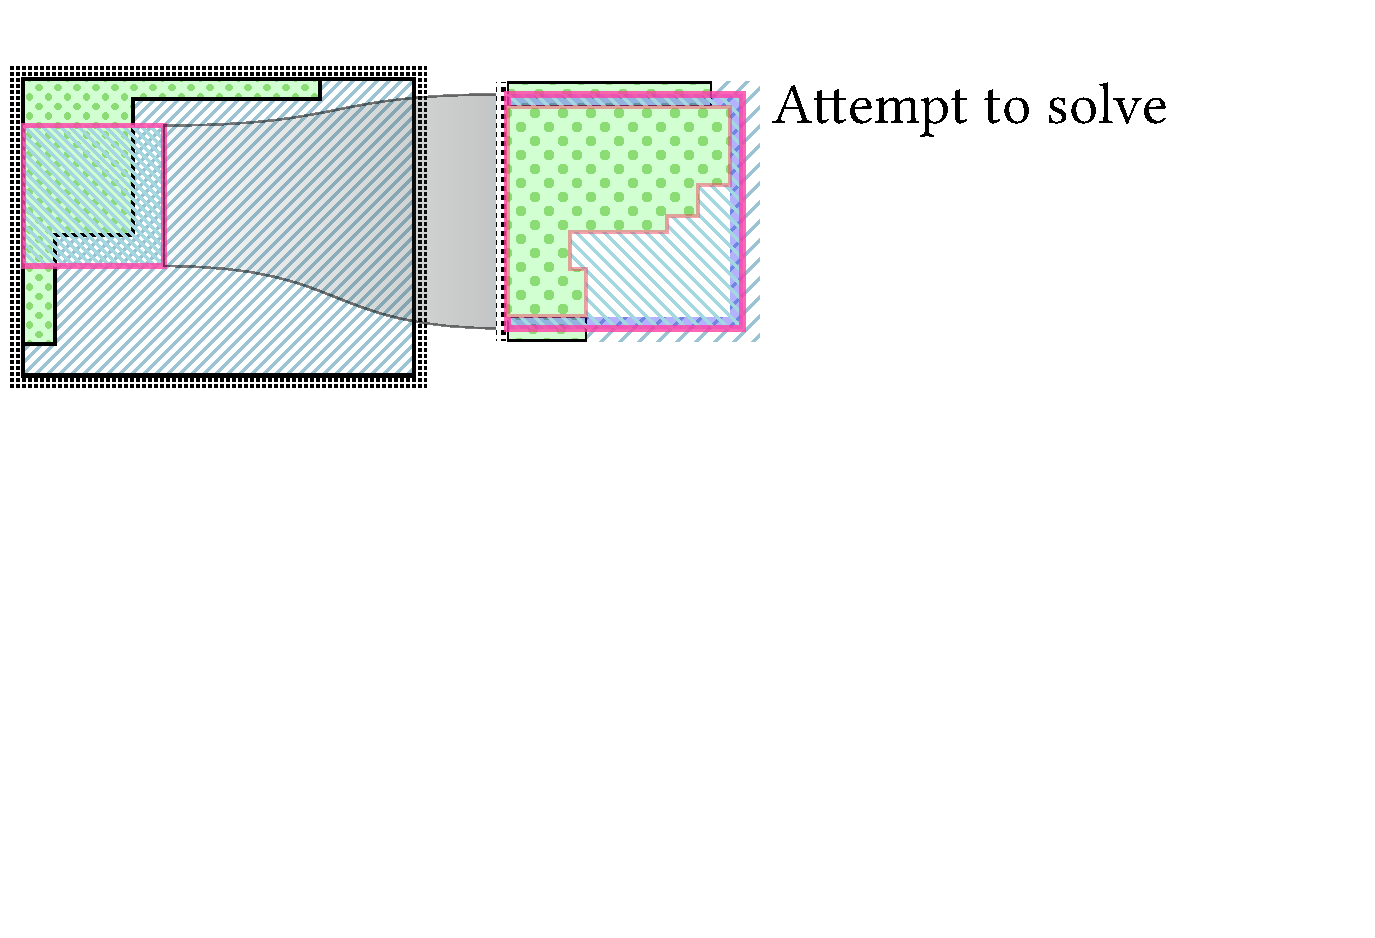
\includegraphics[width=\textwidth]{figs/poms_alg3.pdf}
    \end{figure}
  \end{frame}

  \begin{frame}[fragile]{Algorithm}
    \begin{figure}
      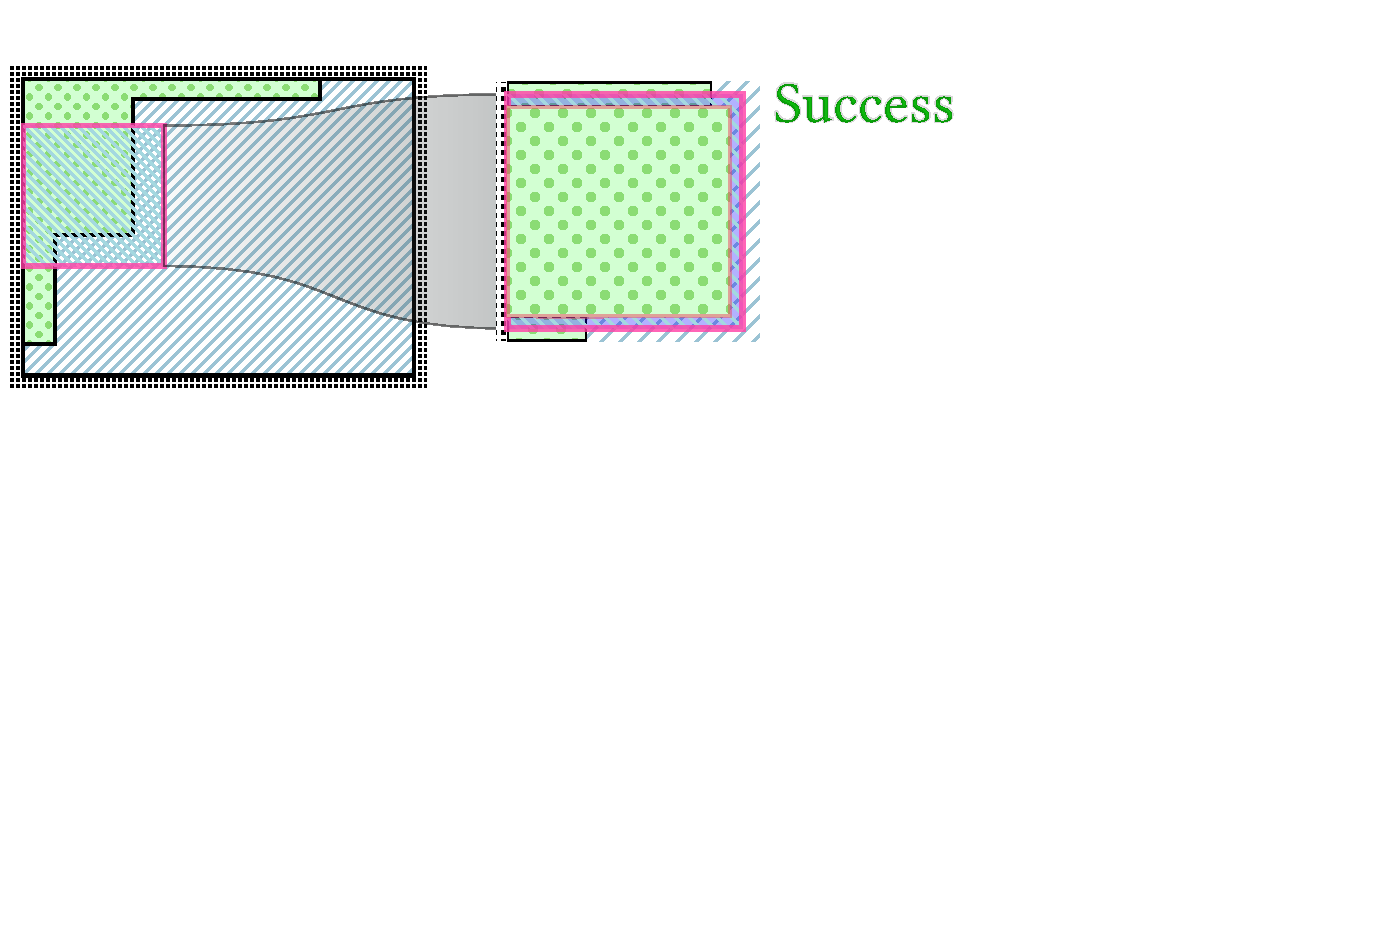
\includegraphics[width=\textwidth]{figs/poms_alg4.pdf}
    \end{figure}
  \end{frame}

  \begin{frame}[fragile]{Algorithm}
    \begin{figure}
      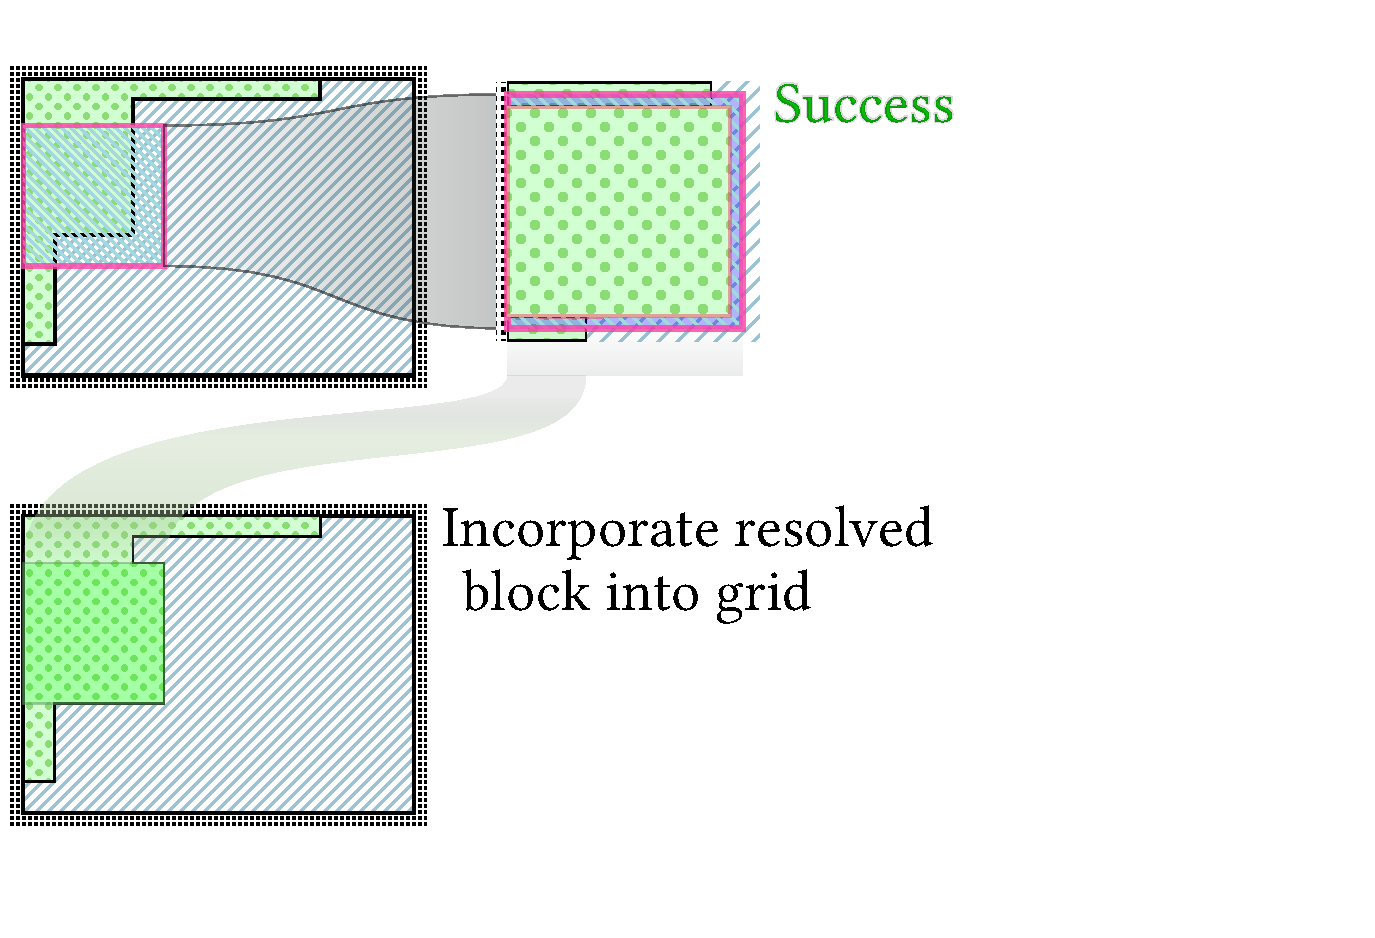
\includegraphics[width=\textwidth]{figs/poms_alg4_5.pdf}
    \end{figure}
  \end{frame}

  \begin{frame}[fragile]{Algorithm}
    \begin{figure}
      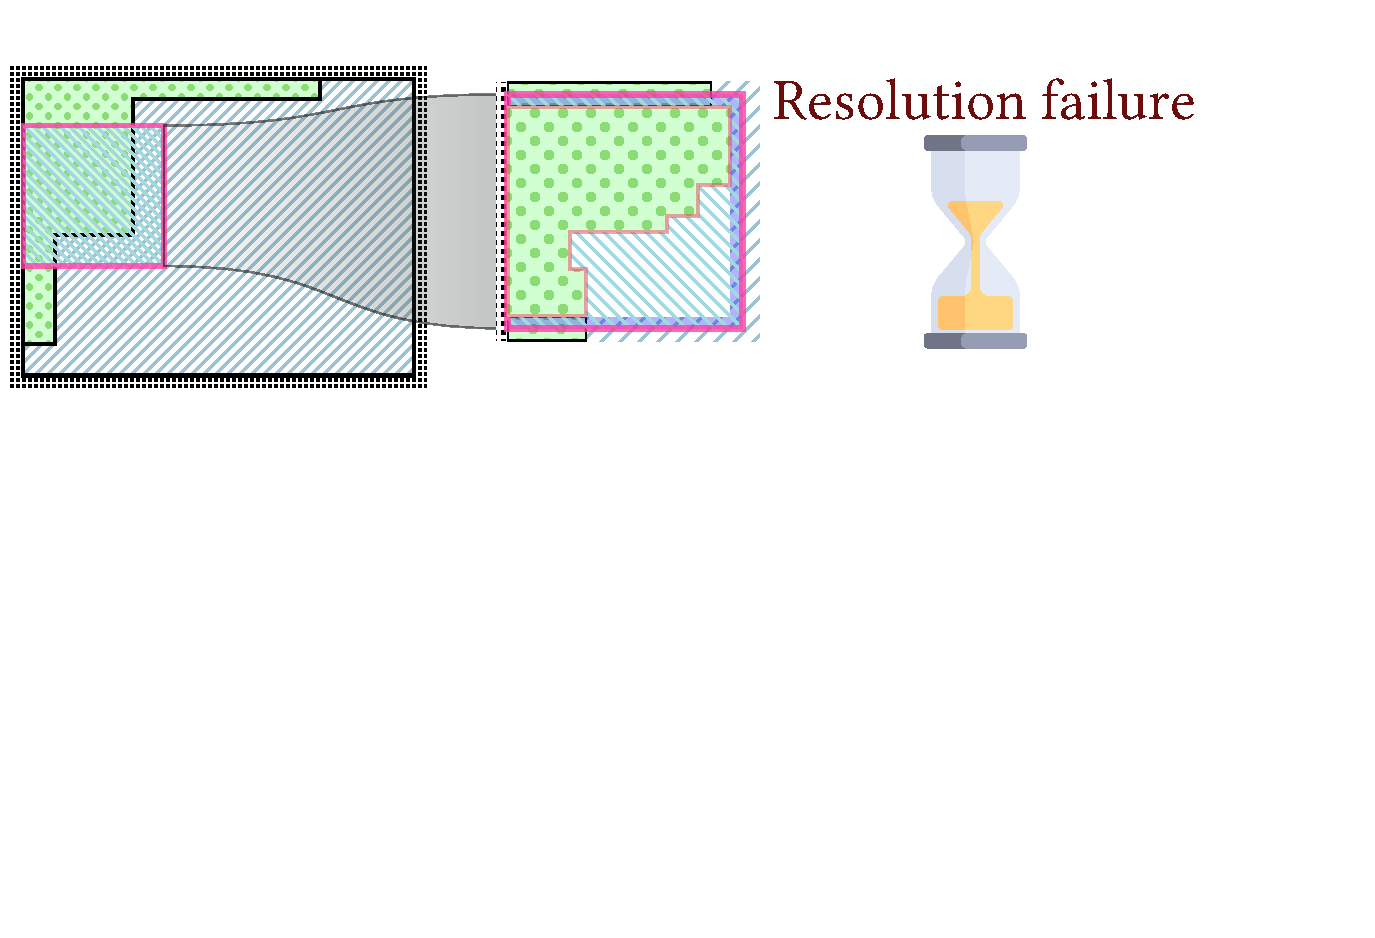
\includegraphics[width=\textwidth]{figs/poms_alg5.pdf}
    \end{figure}
  \end{frame}

  \begin{frame}[fragile]{Algorithm}
    \begin{figure}
      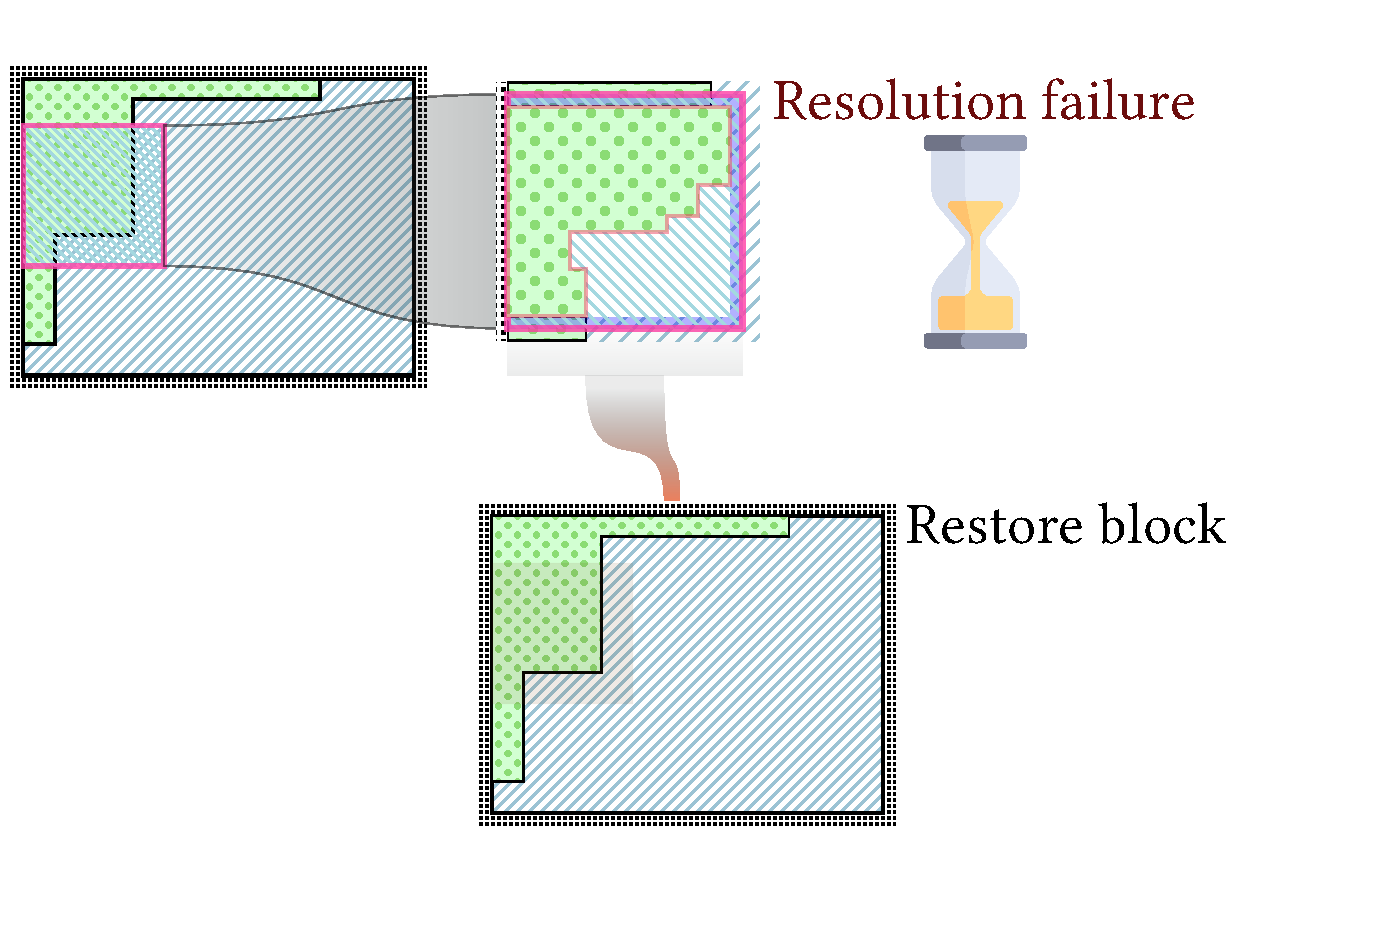
\includegraphics[width=\textwidth]{figs/poms_alg5_1.pdf}
    \end{figure}
  \end{frame}

  \begin{frame}[fragile]{Algorithm}
    \begin{figure}
      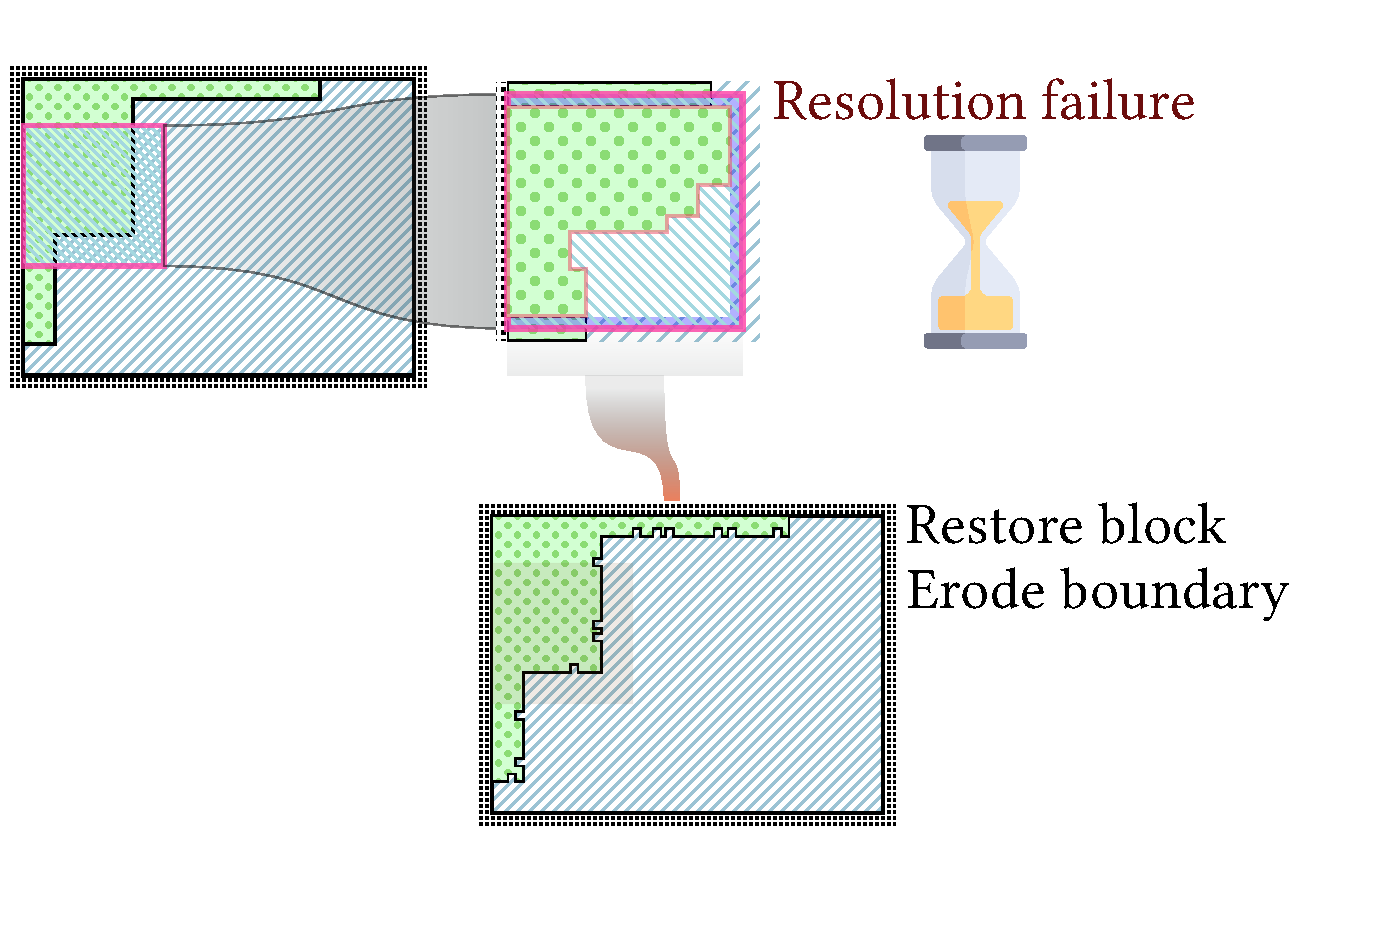
\includegraphics[width=\textwidth]{figs/poms_alg5_2.pdf}
    \end{figure}
  \end{frame}

  \begin{frame}[fragile]{Algorithm}
    \begin{figure}
      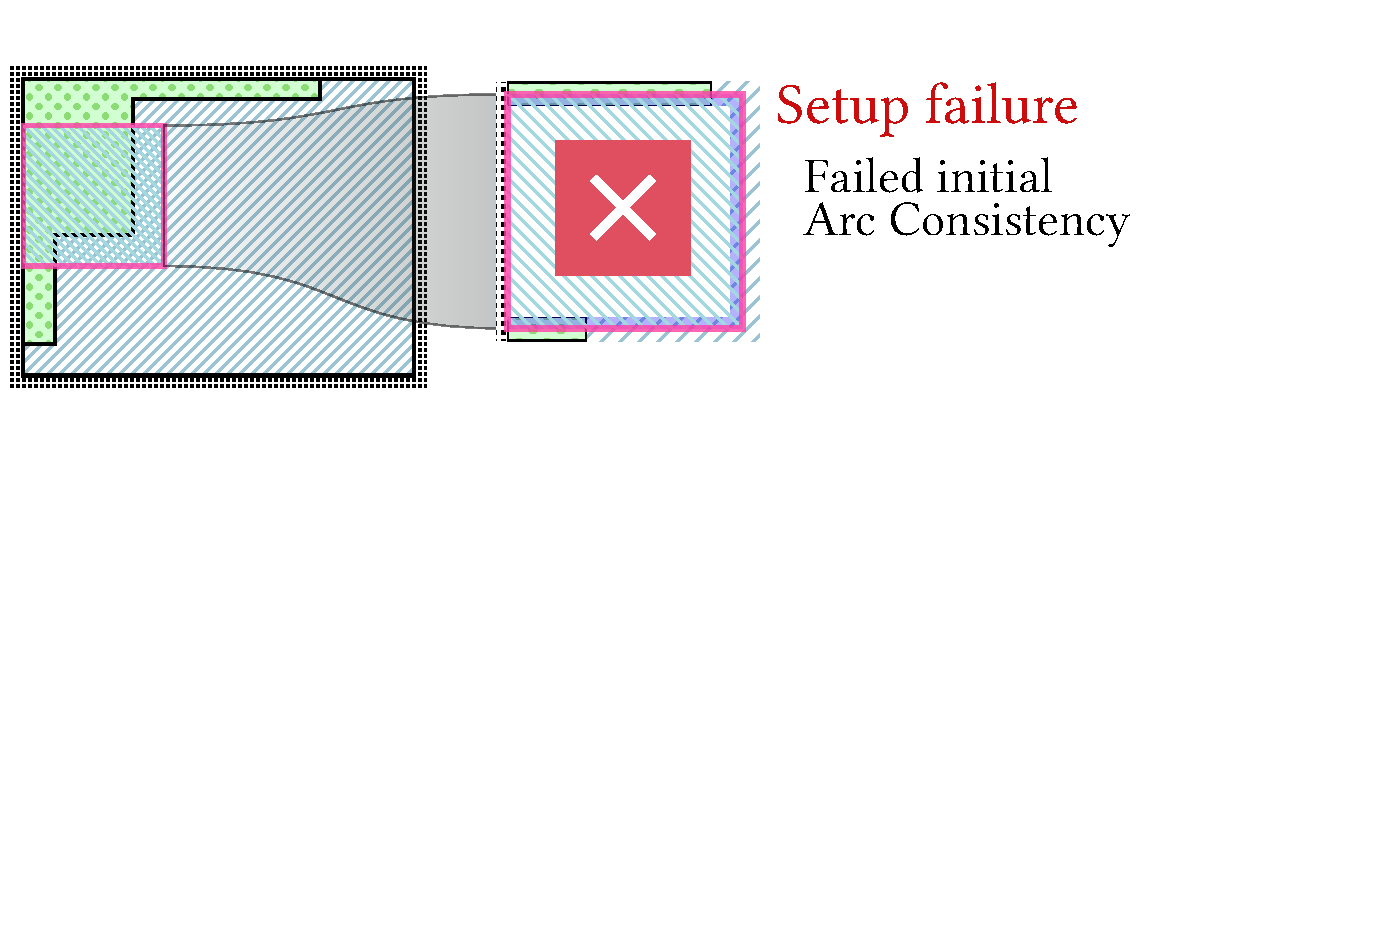
\includegraphics[width=\textwidth]{figs/poms_alg6_1.pdf}
    \end{figure}
  \end{frame}

  \begin{frame}[fragile]{Algorithm}
    \begin{figure}
      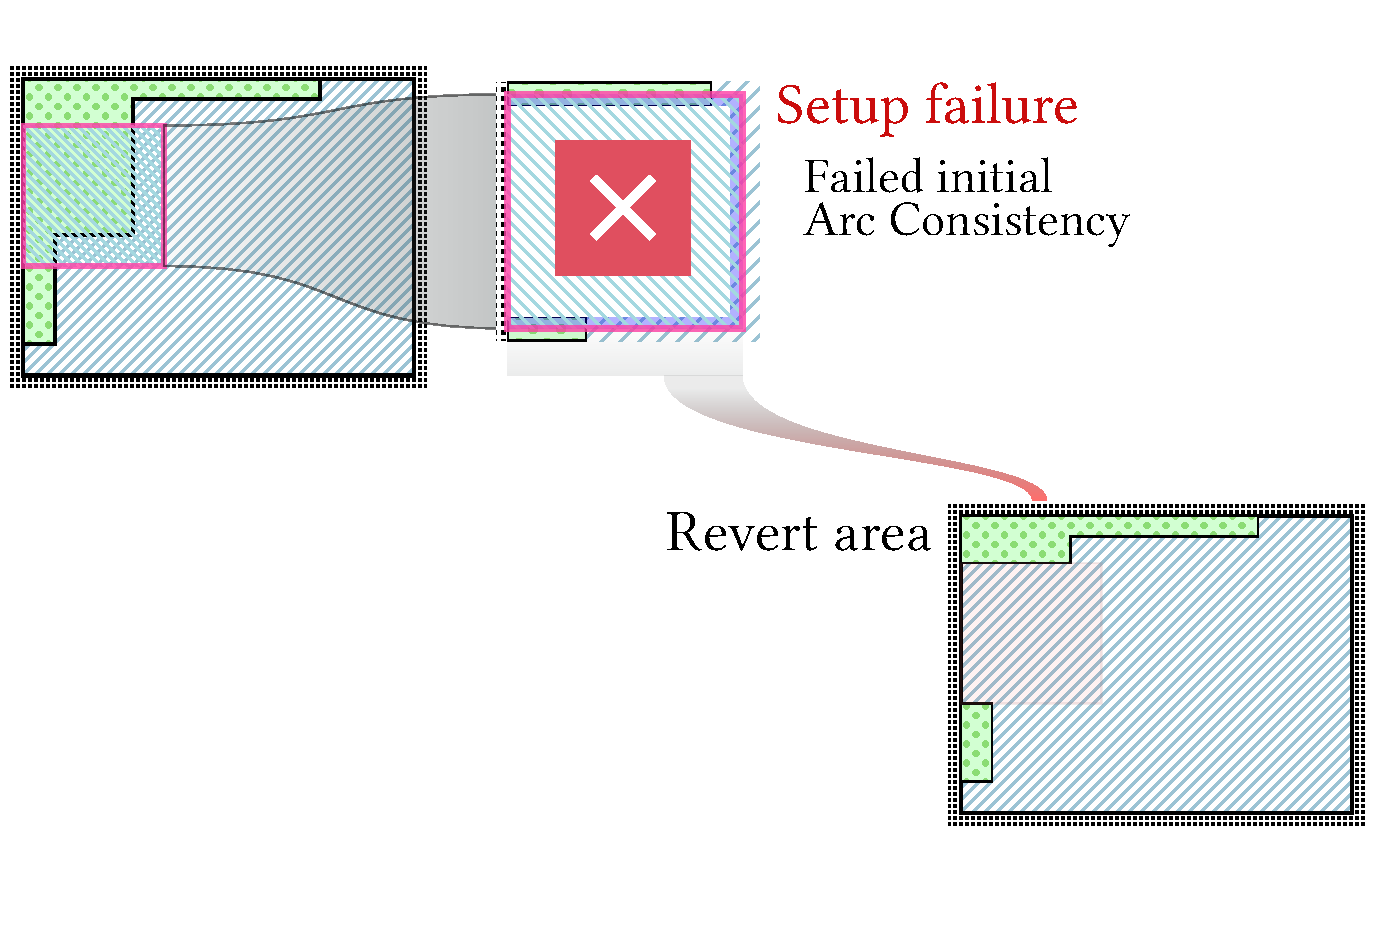
\includegraphics[width=\textwidth]{figs/poms_alg6_2.pdf}
    \end{figure}
  \end{frame}

  \begin{frame}[fragile]{Algorithm}
    \begin{figure}
      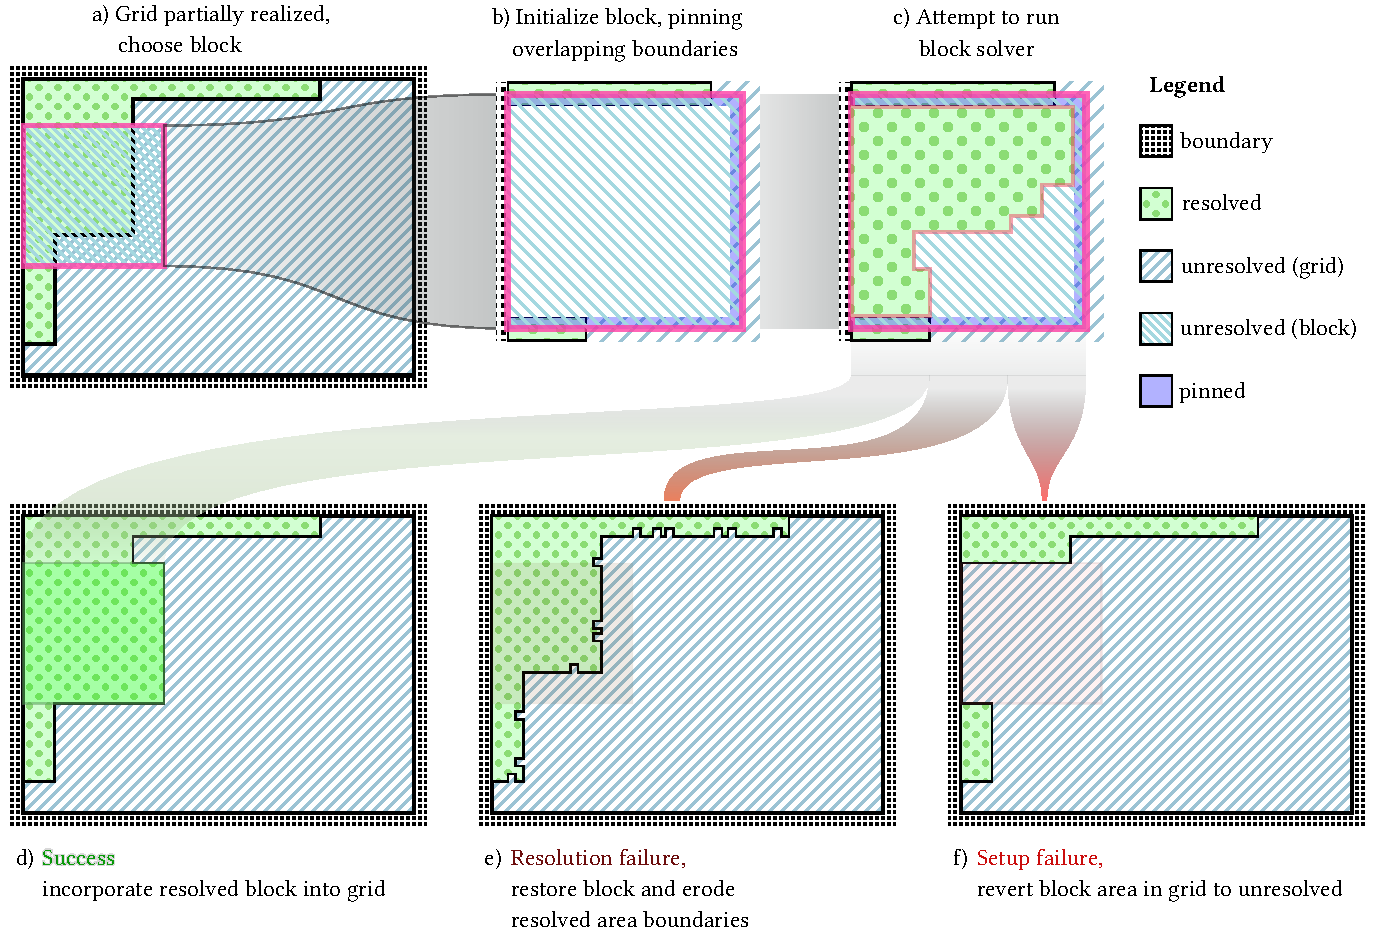
\includegraphics[width=\textwidth]{figs/poms_figalg.pdf}
    \end{figure}
  \end{frame}

  \begin{frame}[fragile]{Algorithm}
    \begin{figure}
      \textit{Pill Mortal} Tile Set

      \movie[width=6cm,height=6cm,poster,autostart,repeat]{}{vid/pm_w.mp4}
    \end{figure}
  \end{frame}

%  \begin{frame}[fragile]{Algorithm}
%    \begin{figure}
%      LUNARSIGNALS' \textit{Overhead Action RPG Overworld} Tile Set
%
%      \movie[width=6cm,height=6cm,poster,autostart,repeat]{}{vid/oarpgo_x10_w.mp4}
%    \end{figure}
%  \end{frame}

  \begin{frame}[fragile]{Algorithm}

    \begin{figure}
      ThKaspar's \textit{Forest Micro} Tile Set

      \movie[width=6cm,height=6cm,poster,autostart,repeat]{}{vid/forestmicro_x5_w.mp4}
    \end{figure}
  \end{frame}

  \begin{frame}[fragile]{Algorithm}
    \begin{figure}
      Choose Block

      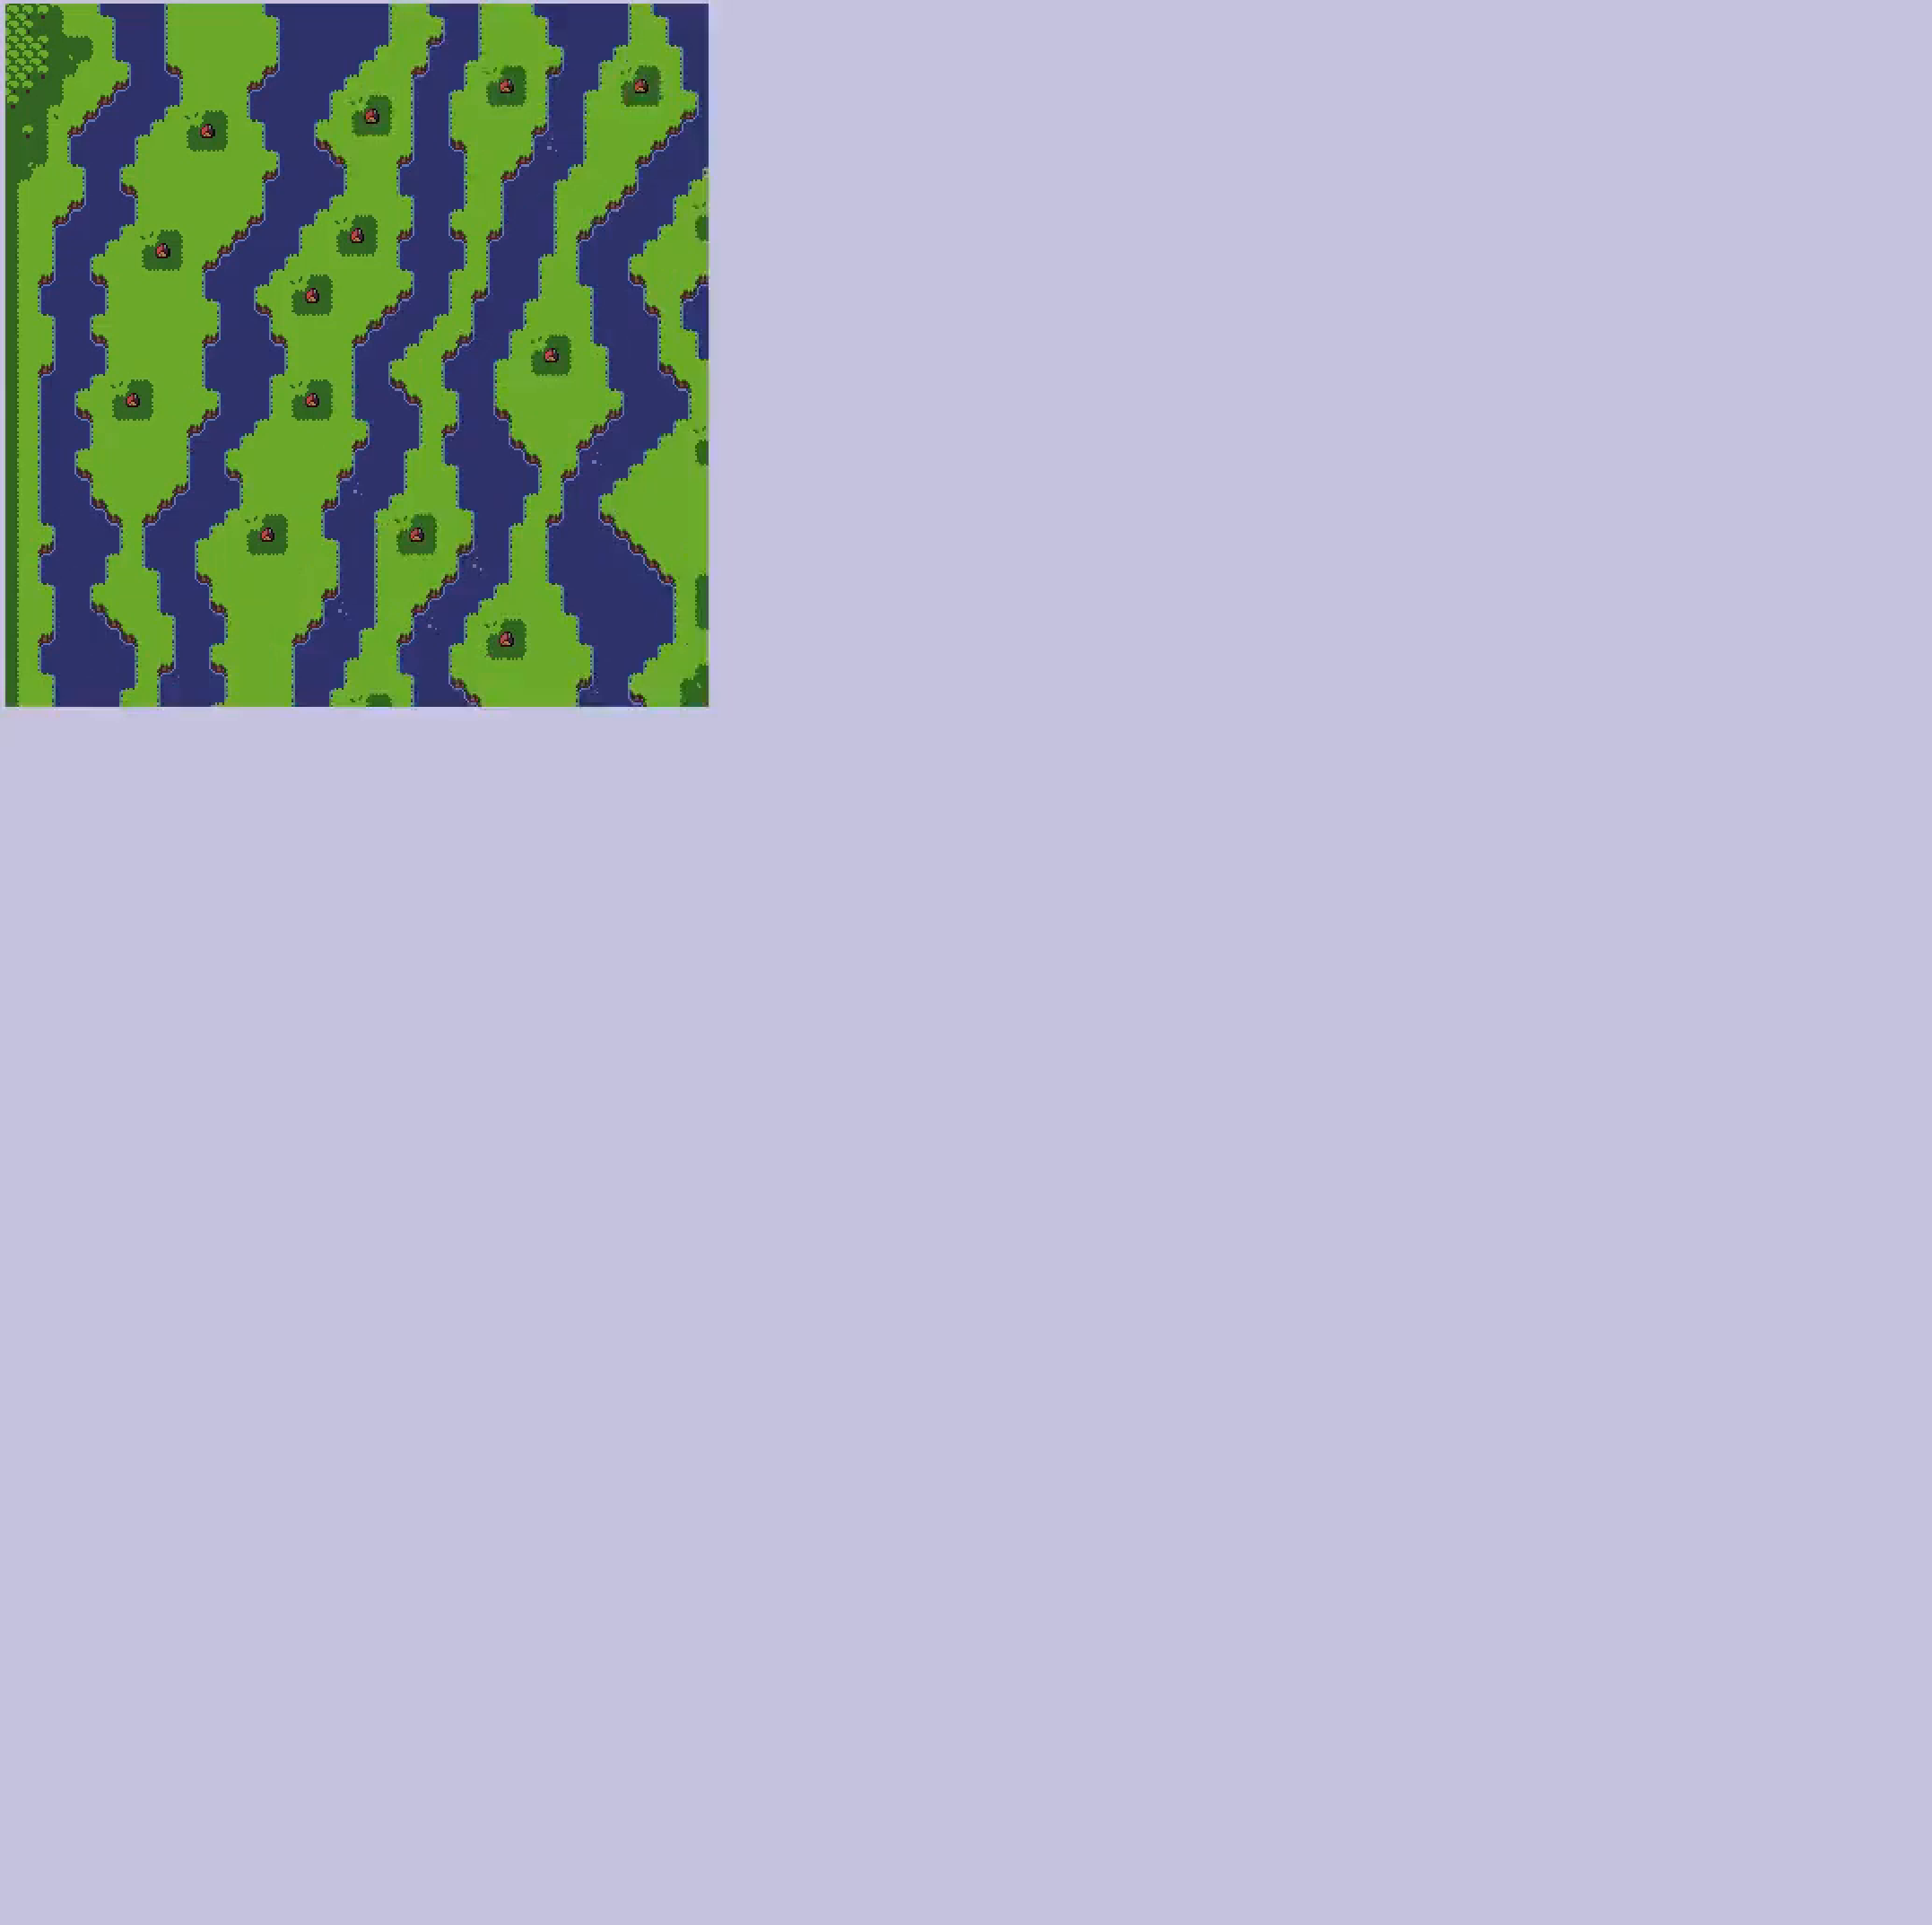
\includegraphics[width=6cm]{img/fm_0005.pdf}
    \end{figure}
  \end{frame}

  \begin{frame}[fragile]{Algorithm}
    \begin{figure}
      Choose Block

      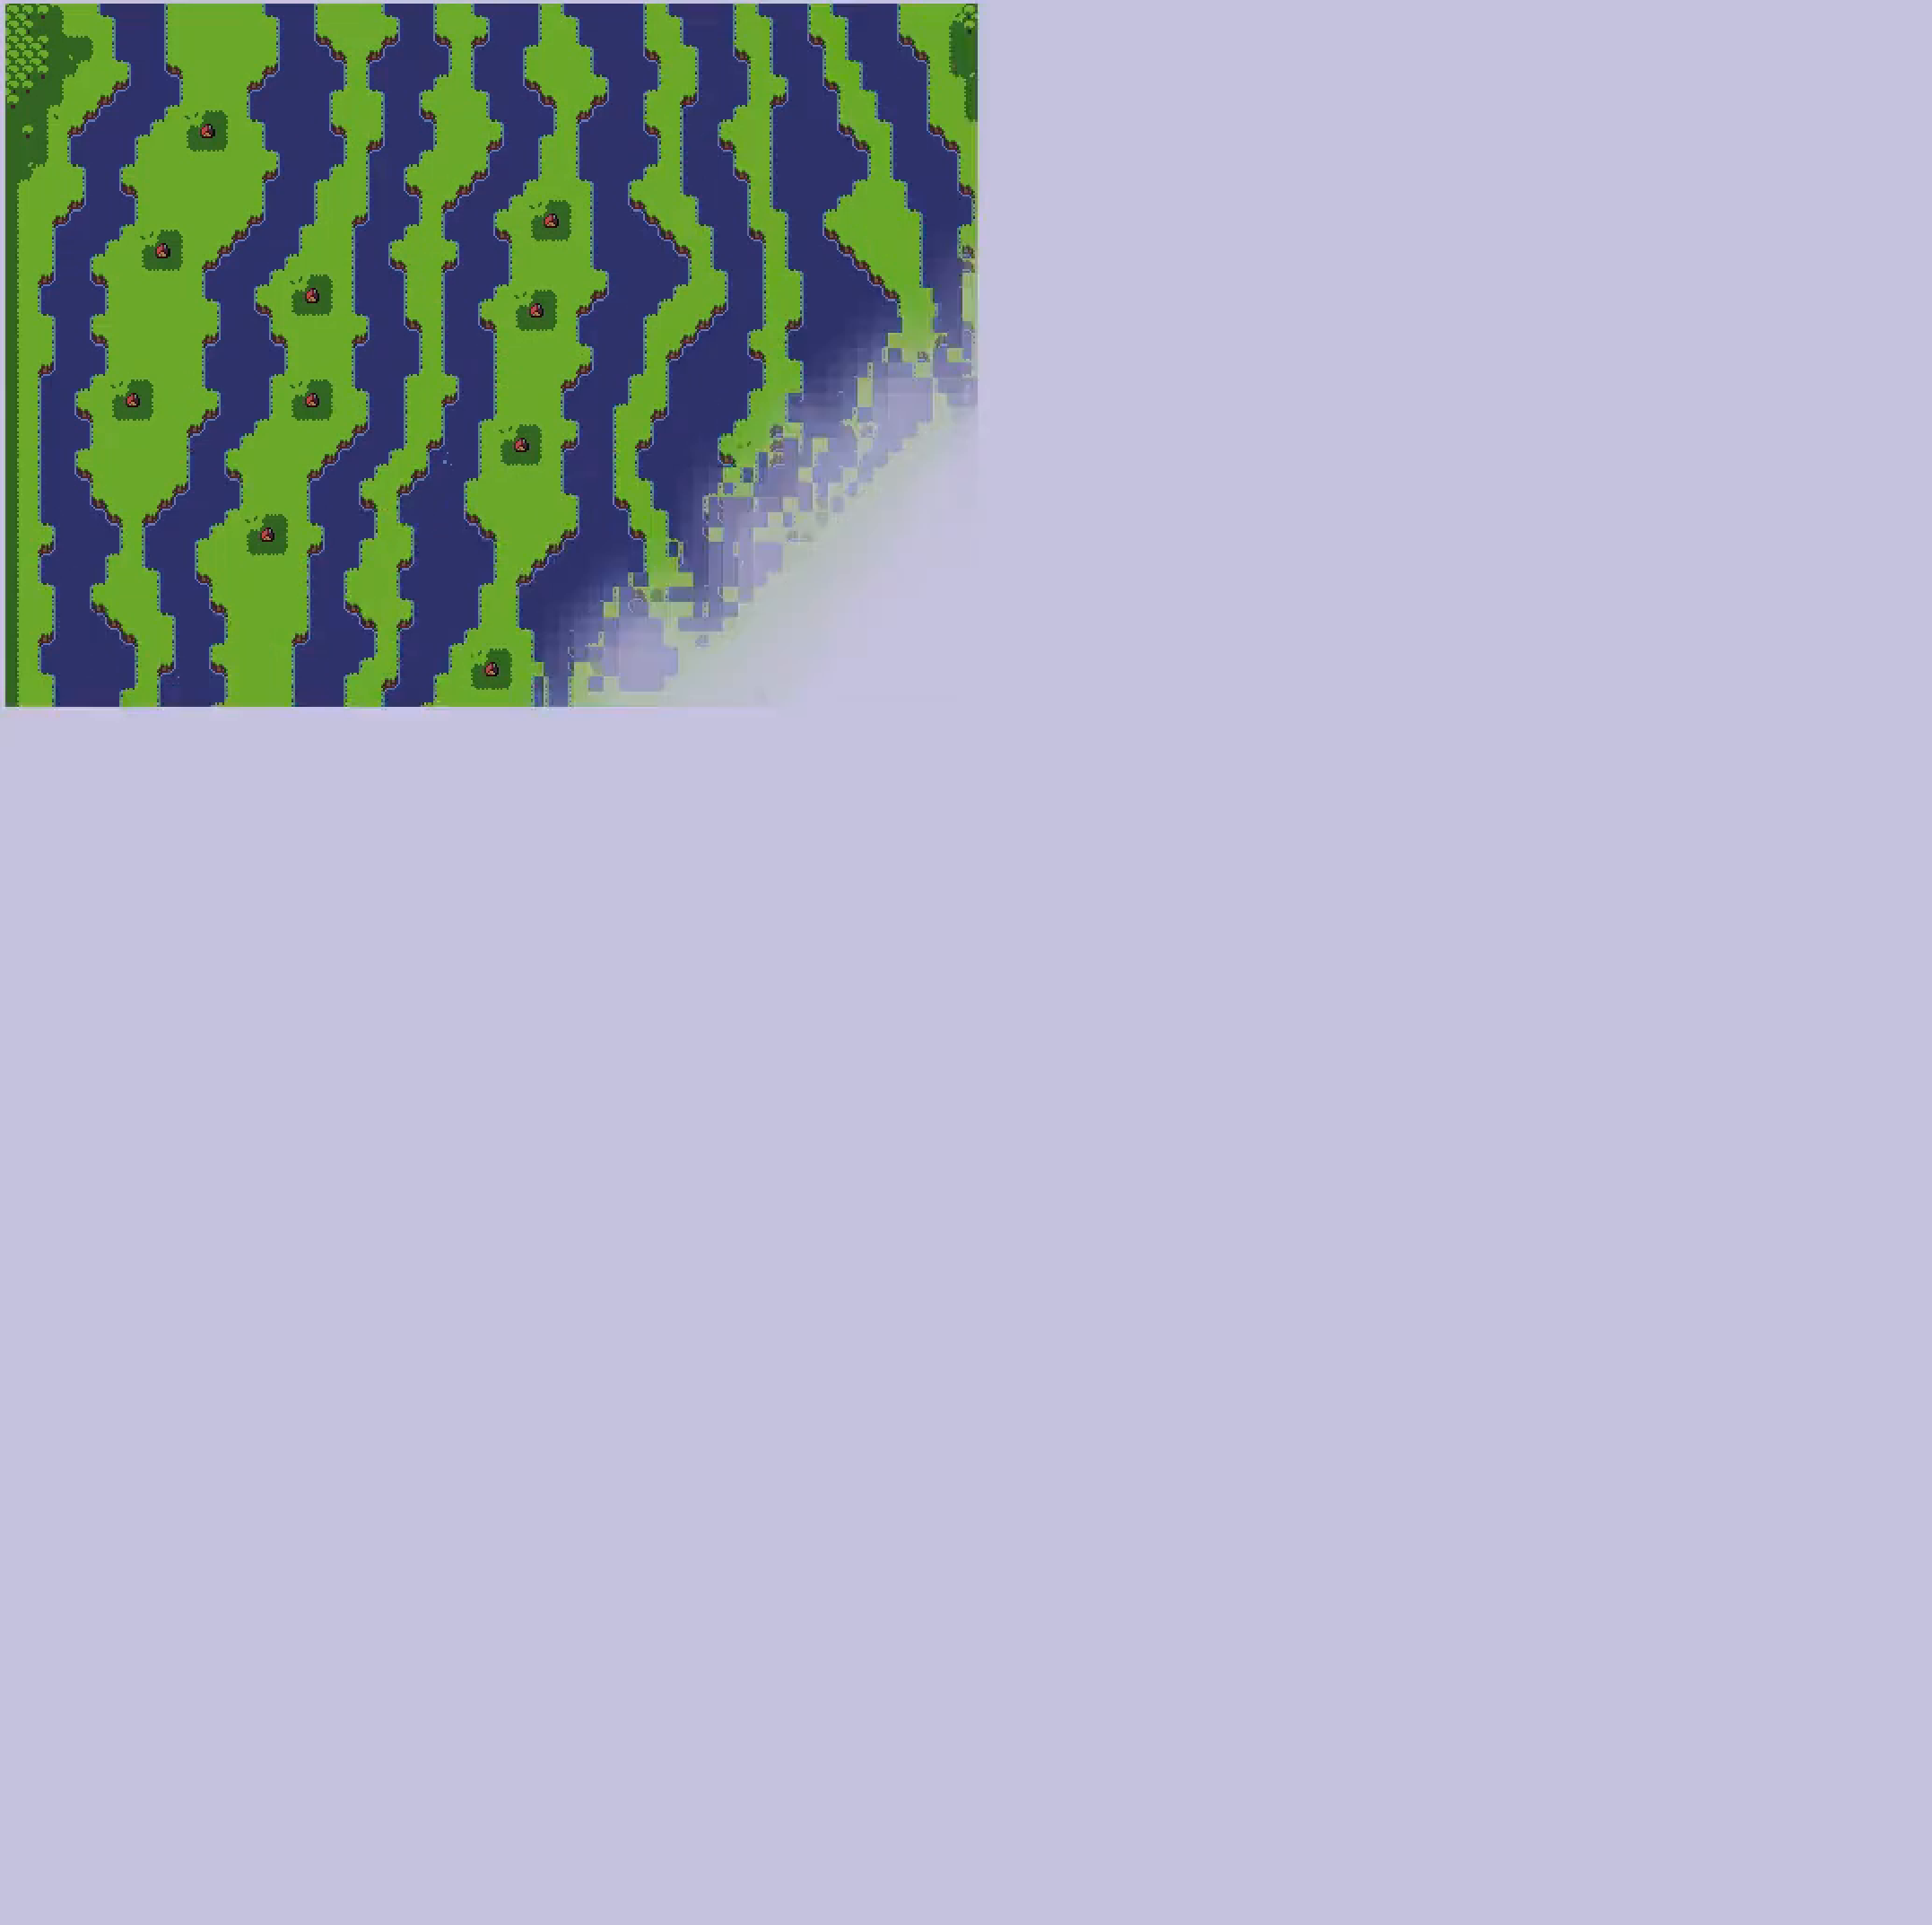
\includegraphics[width=6cm]{img/fm_0006.pdf}
    \end{figure}
  \end{frame}

  \begin{frame}[fragile]{Algorithm}
    \begin{figure}
      Revert Block

      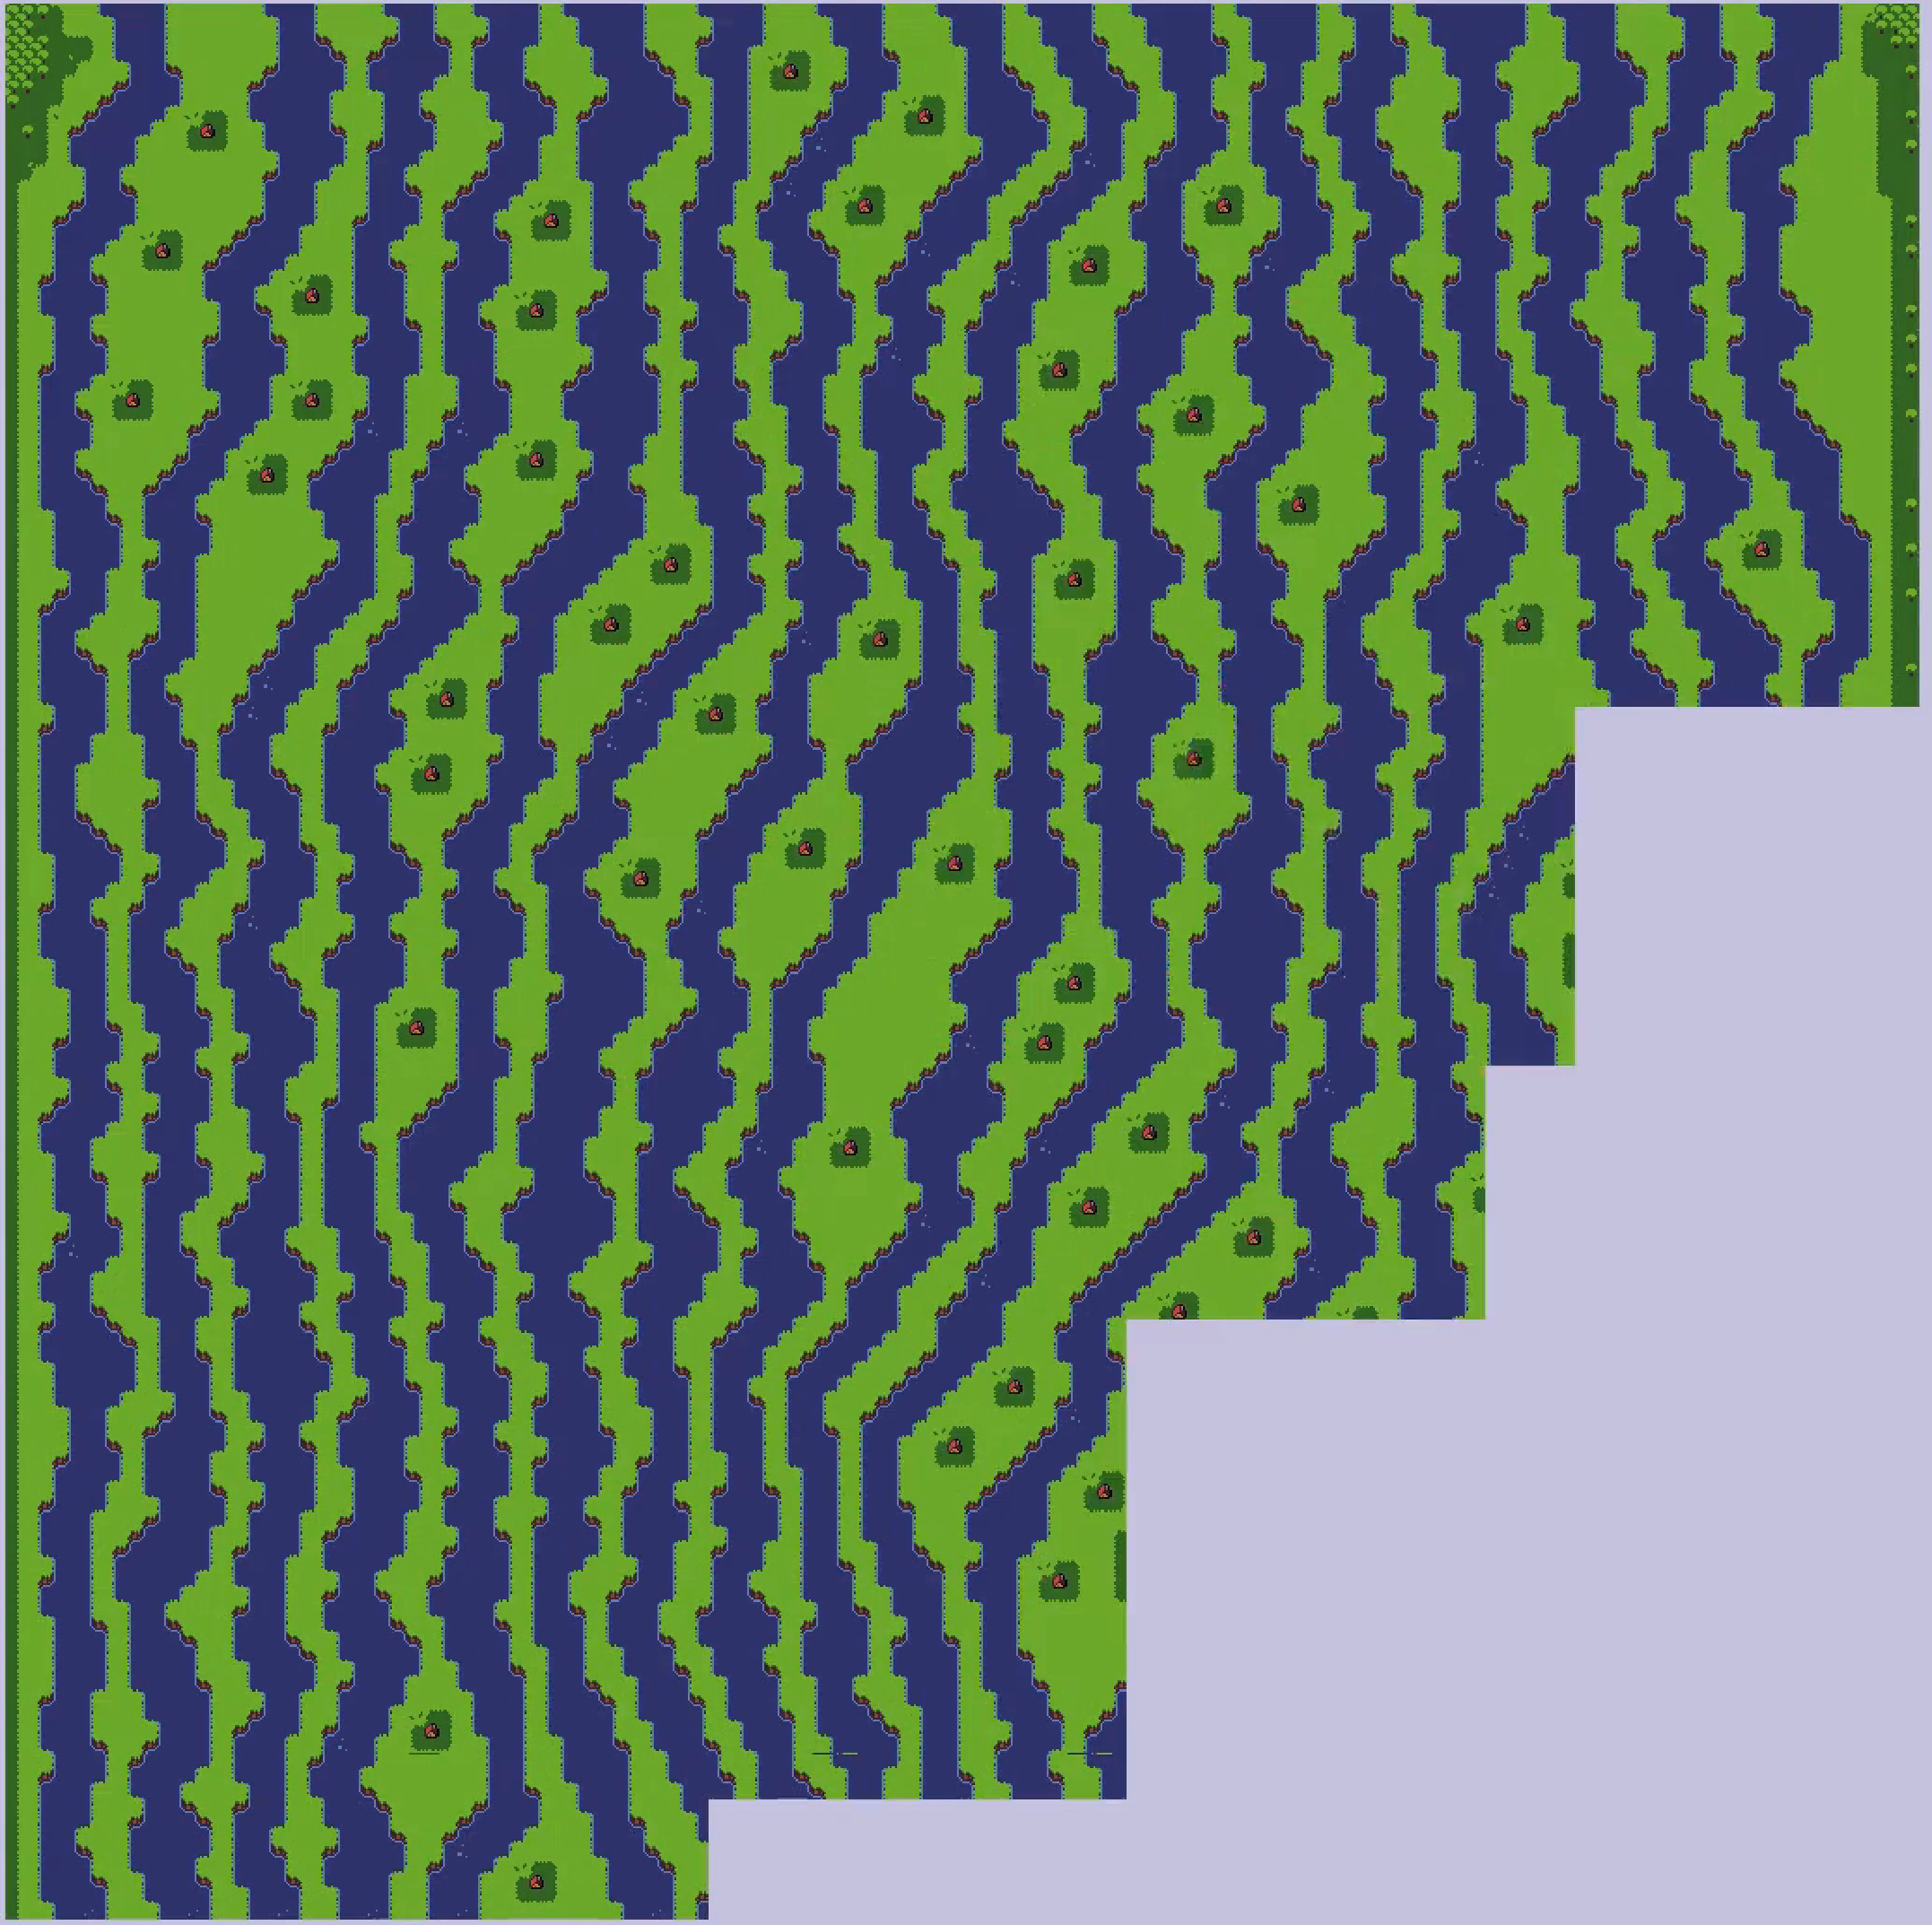
\includegraphics[width=6cm]{img/fm_0023.pdf}
    \end{figure}
  \end{frame}

  \begin{frame}[fragile]{Algorithm}
    \begin{figure}
      Revert Block

      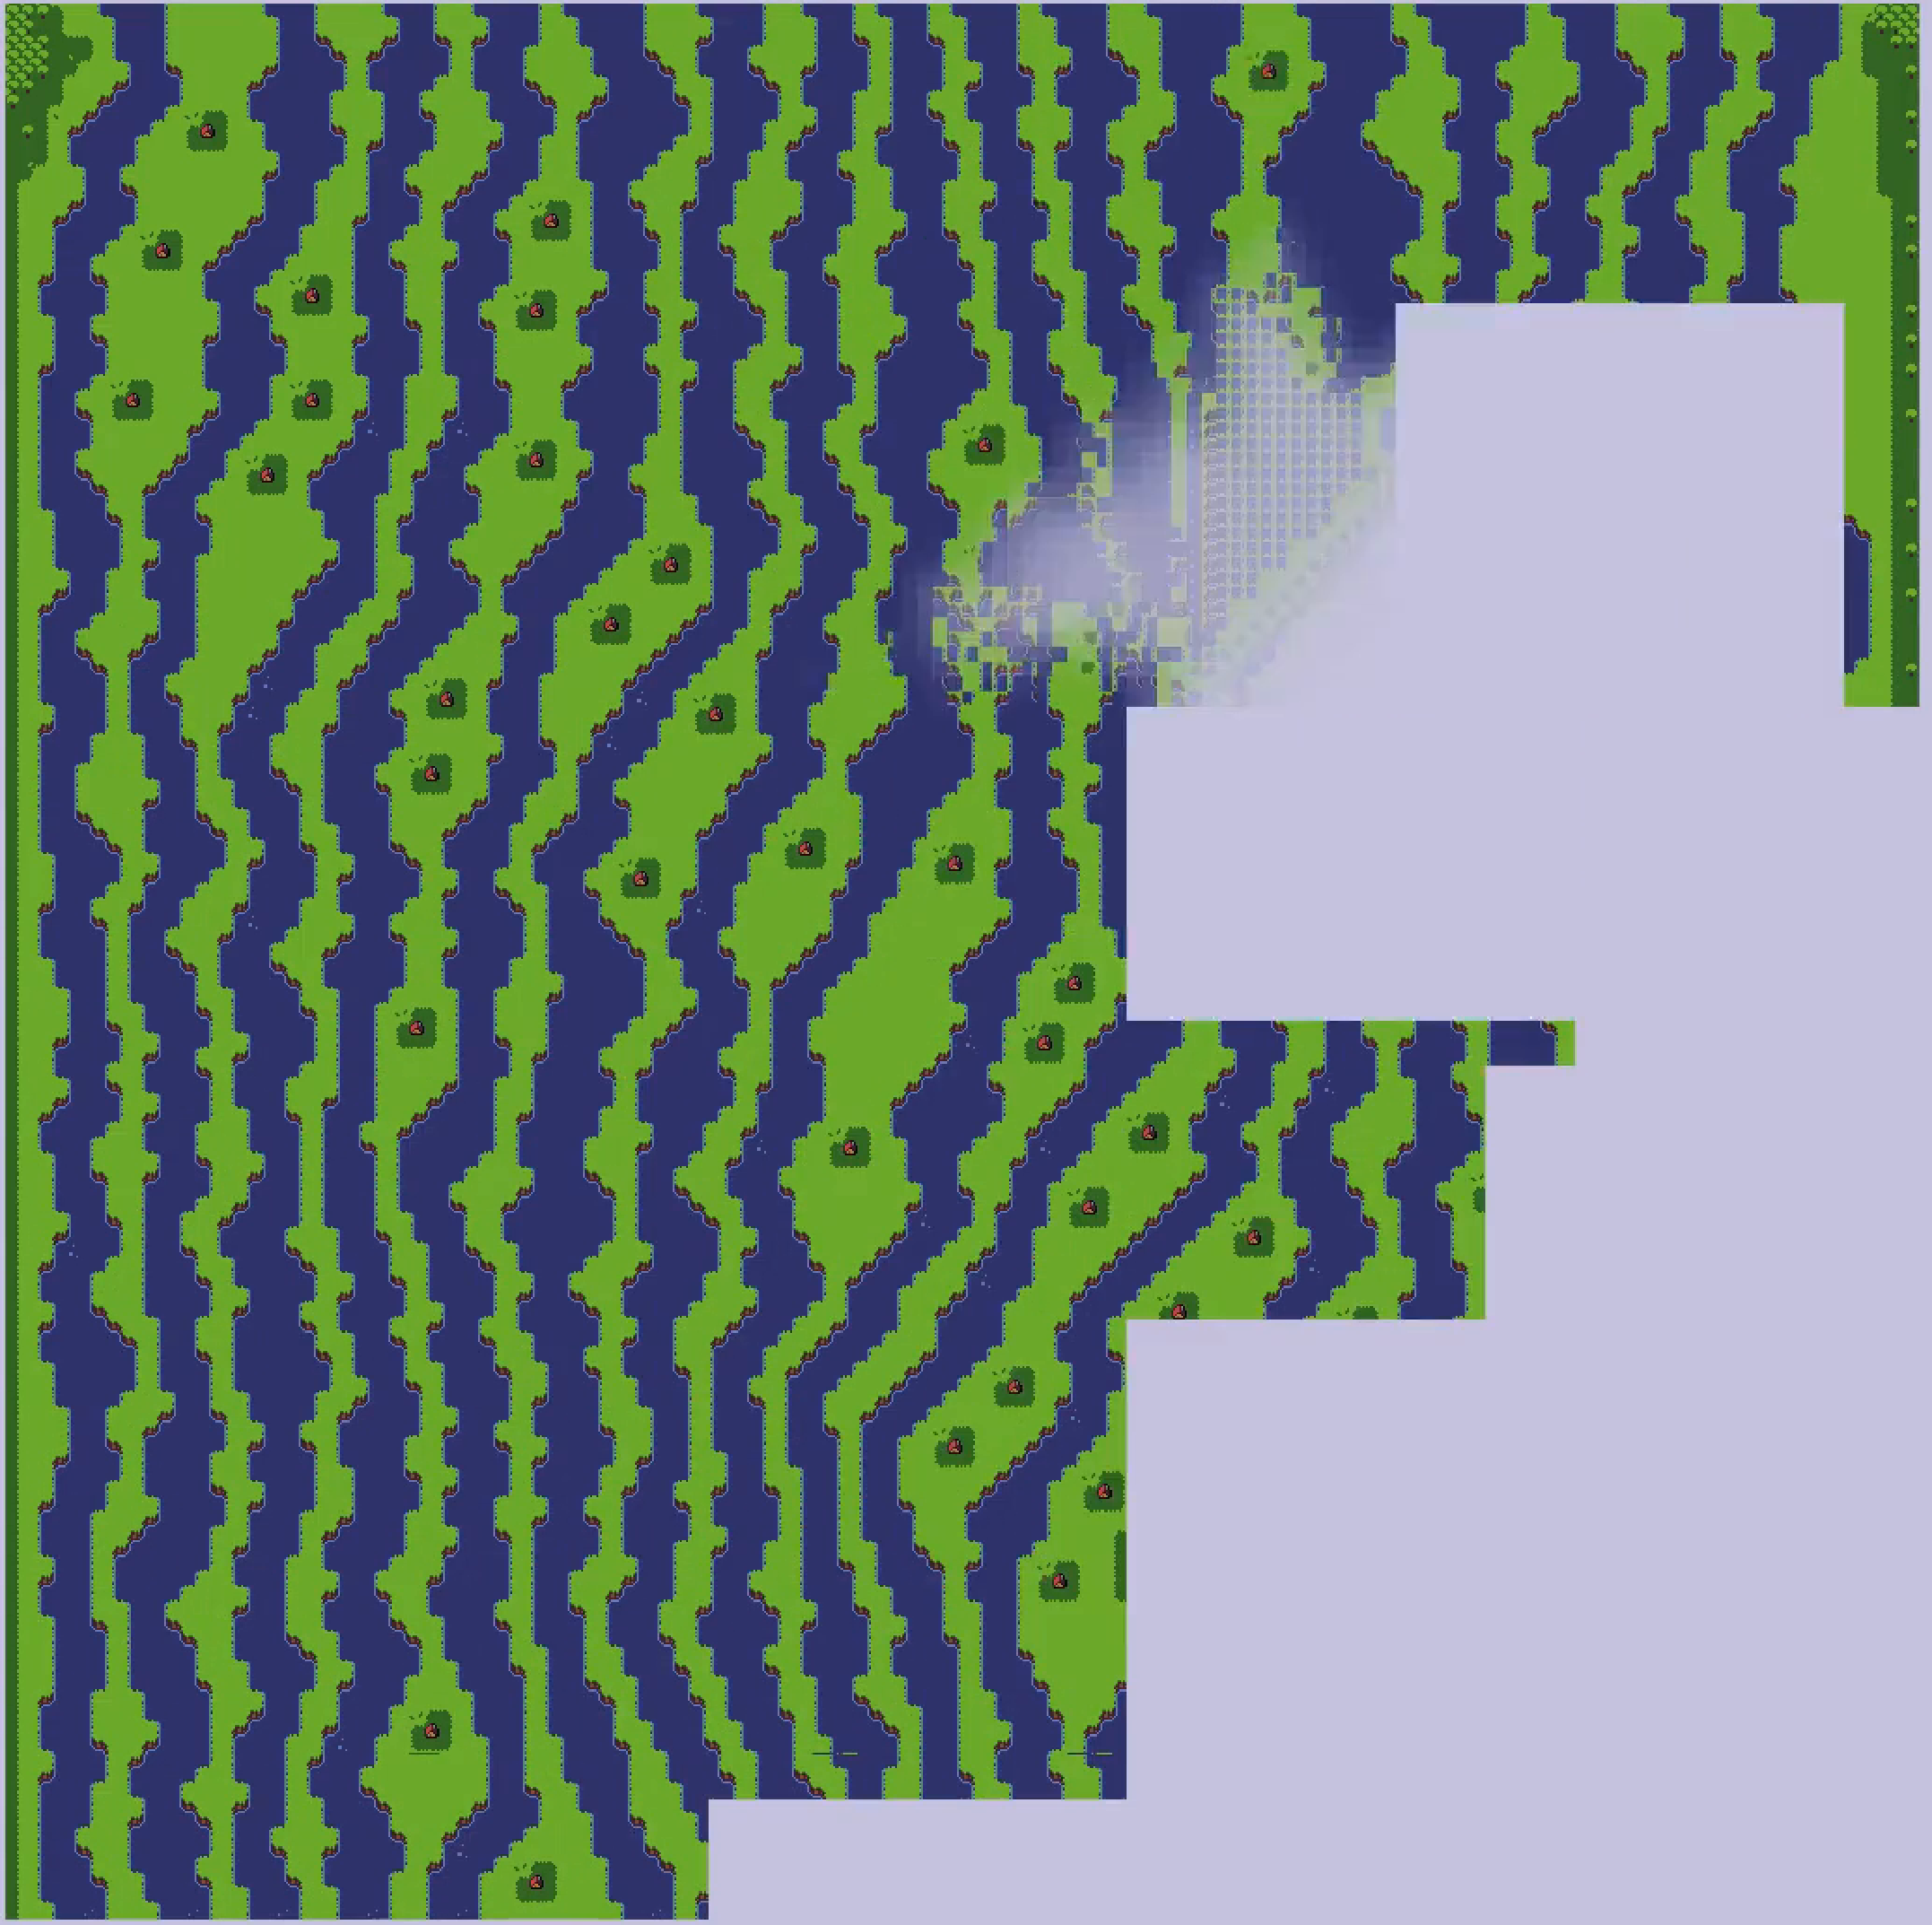
\includegraphics[width=6cm]{img/fm_0024.pdf}
    \end{figure}
  \end{frame}

  \begin{frame}[fragile]{Algorithm}

    \begin{figure}
      Erode Boundary

      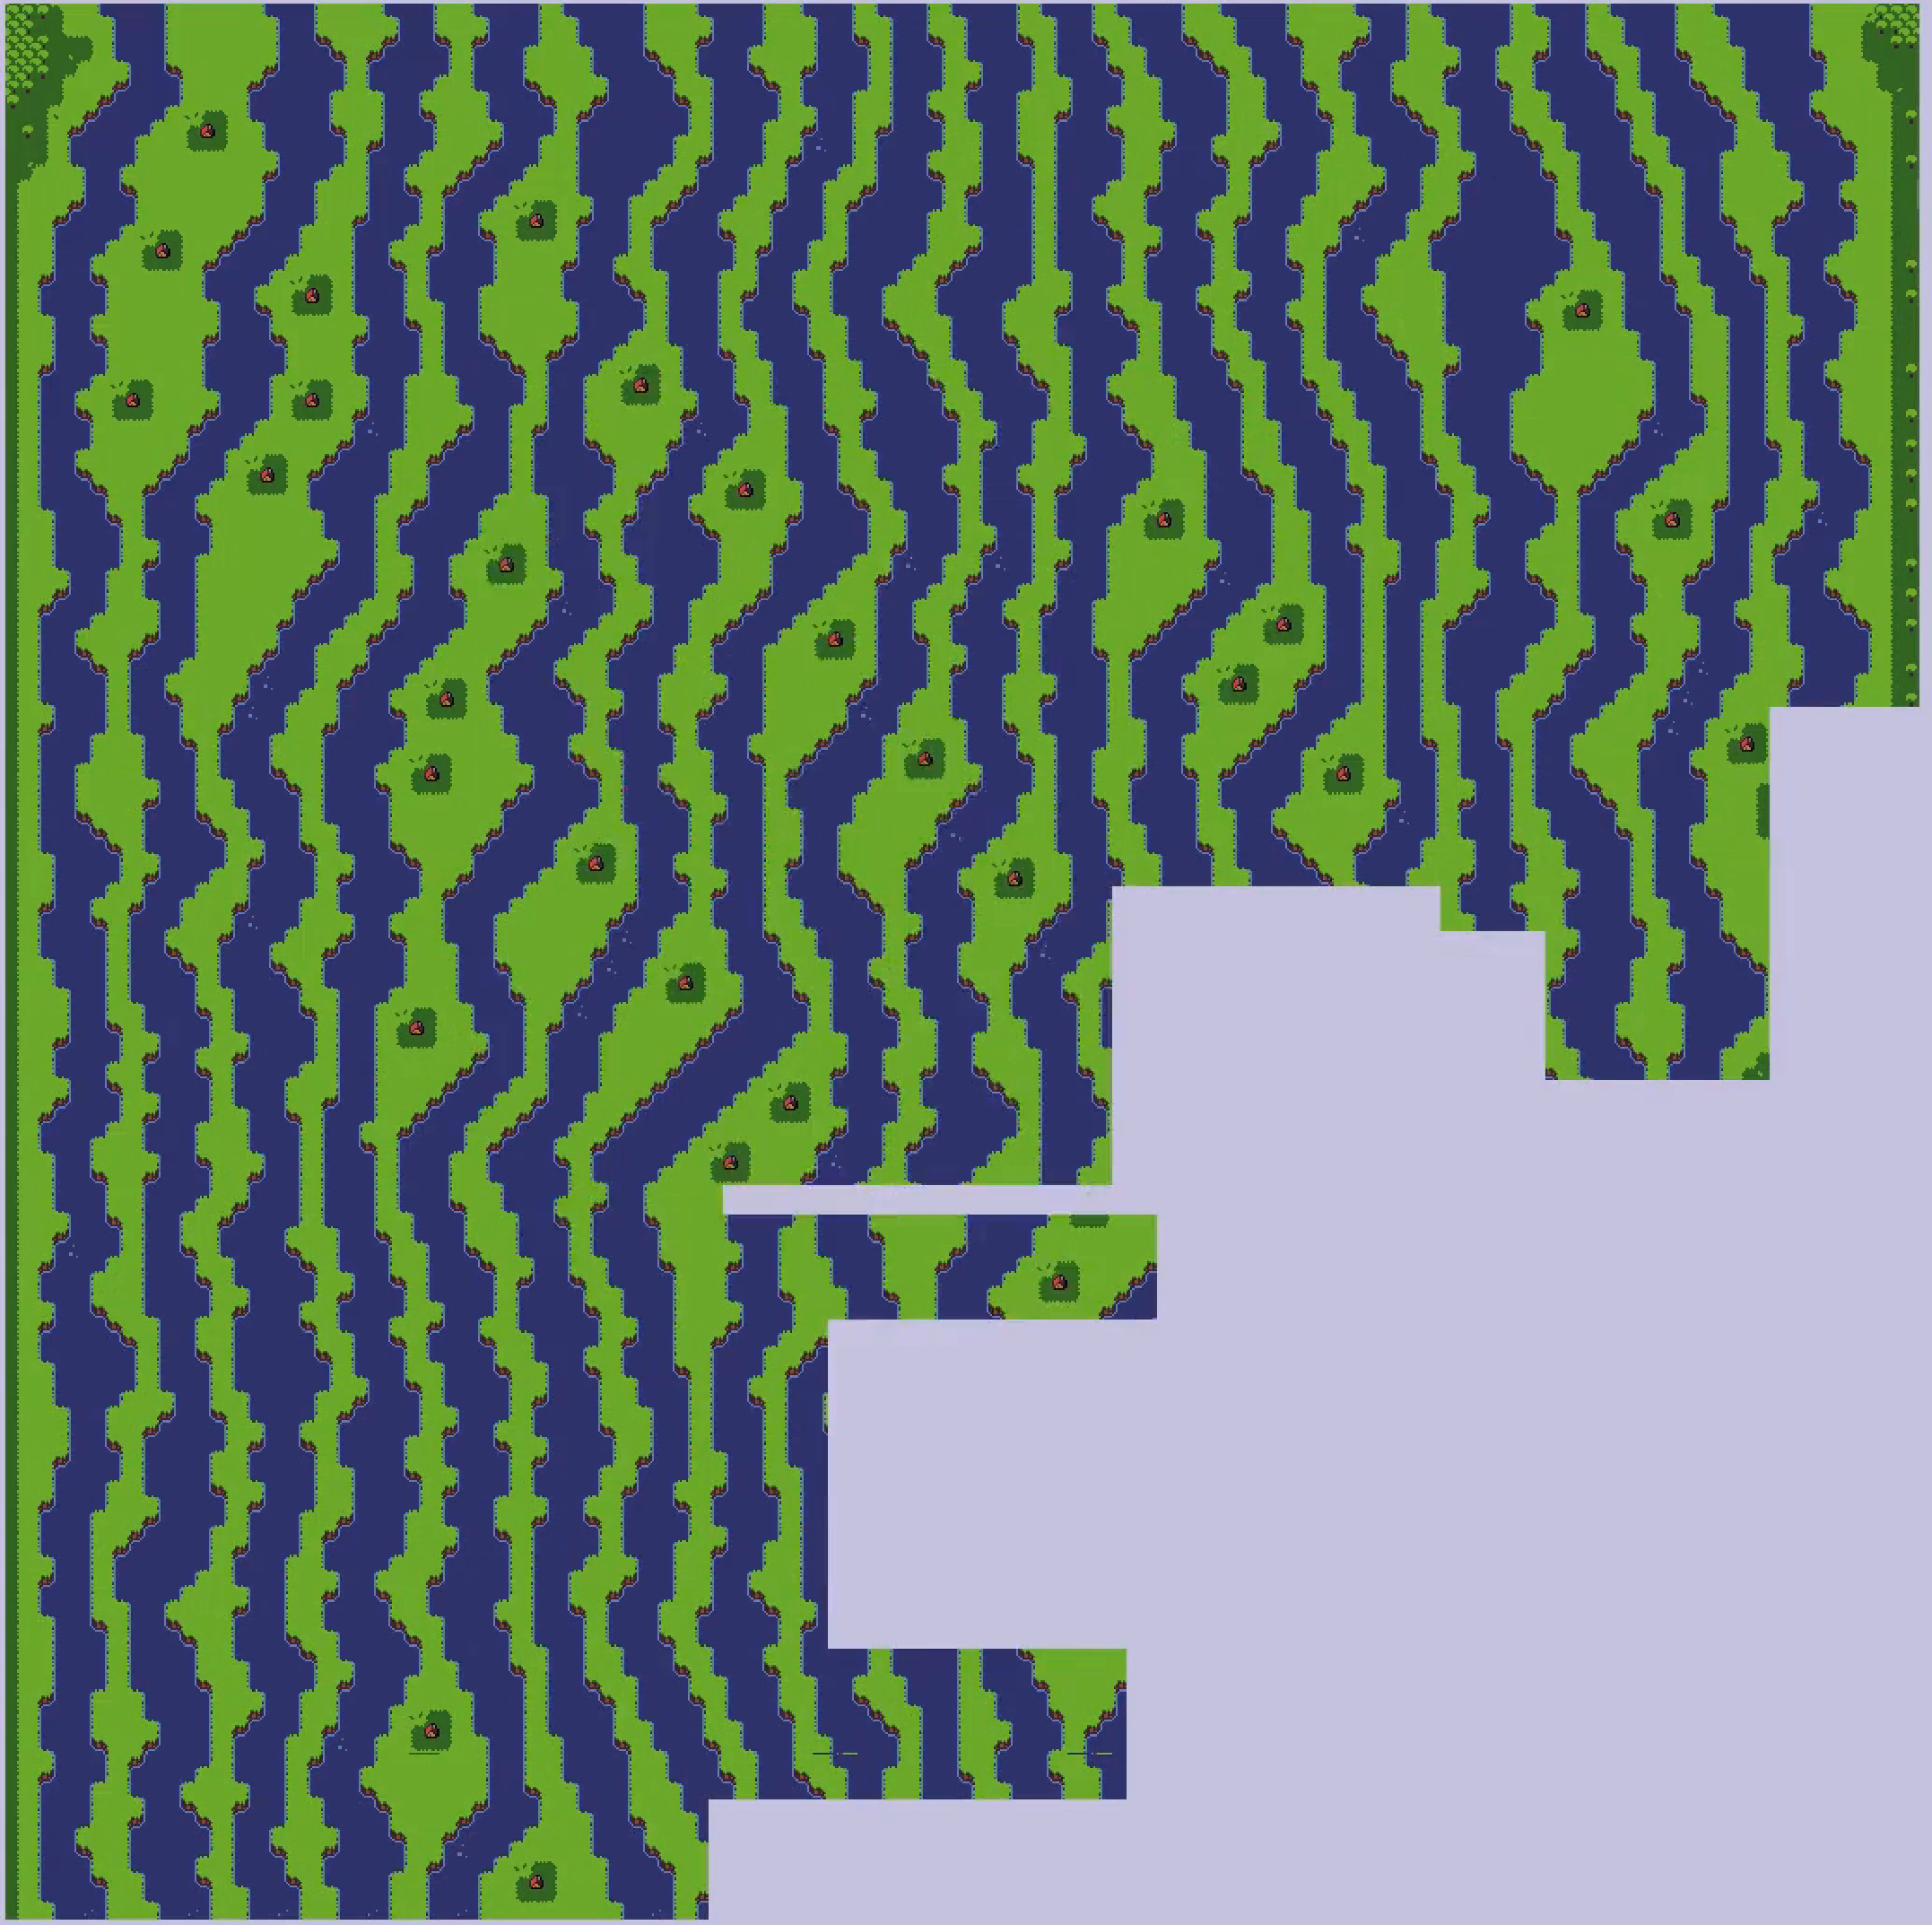
\includegraphics[width=6cm]{img/fm_0035.pdf}
    \end{figure}
  \end{frame}

  \begin{frame}[fragile]{Algorithm}

    \begin{figure}
      Erode Boundary

      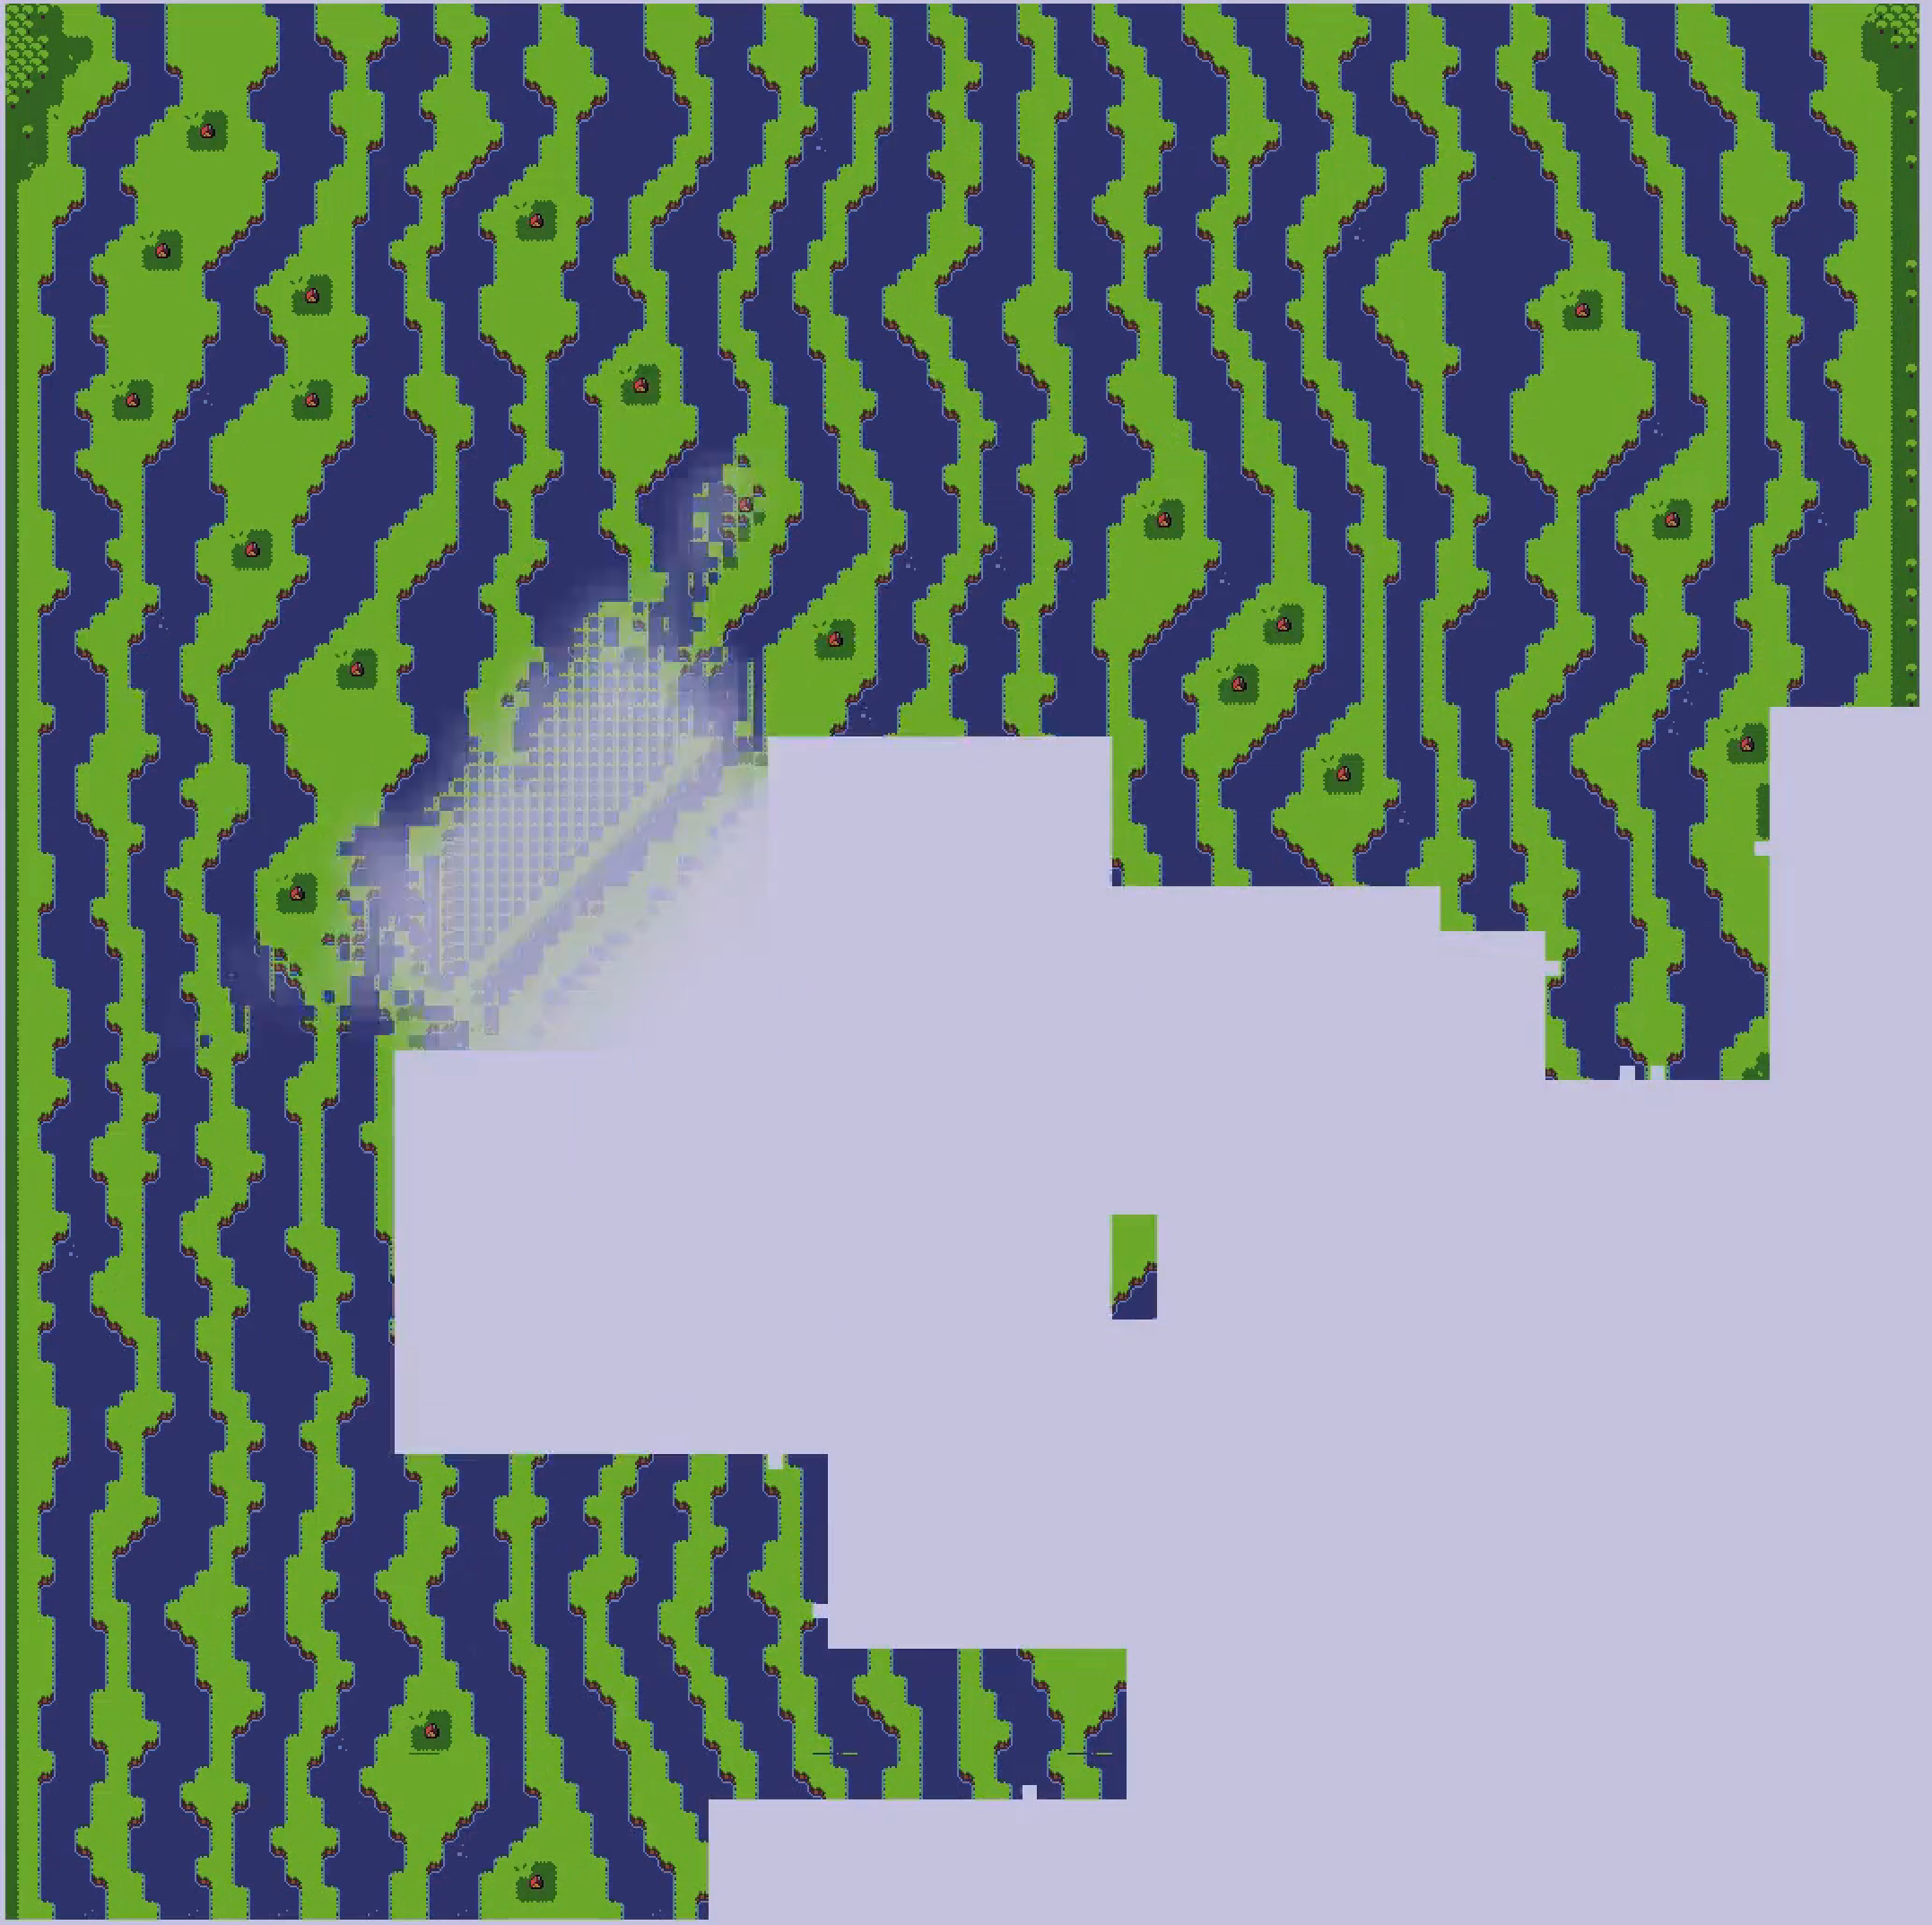
\includegraphics[width=6cm]{img/fm_0036.pdf}
    \end{figure}
  \end{frame}

%  \begin{frame}[fragile]{Algorithm}
%    Choose Block
%    \begin{figure}
%      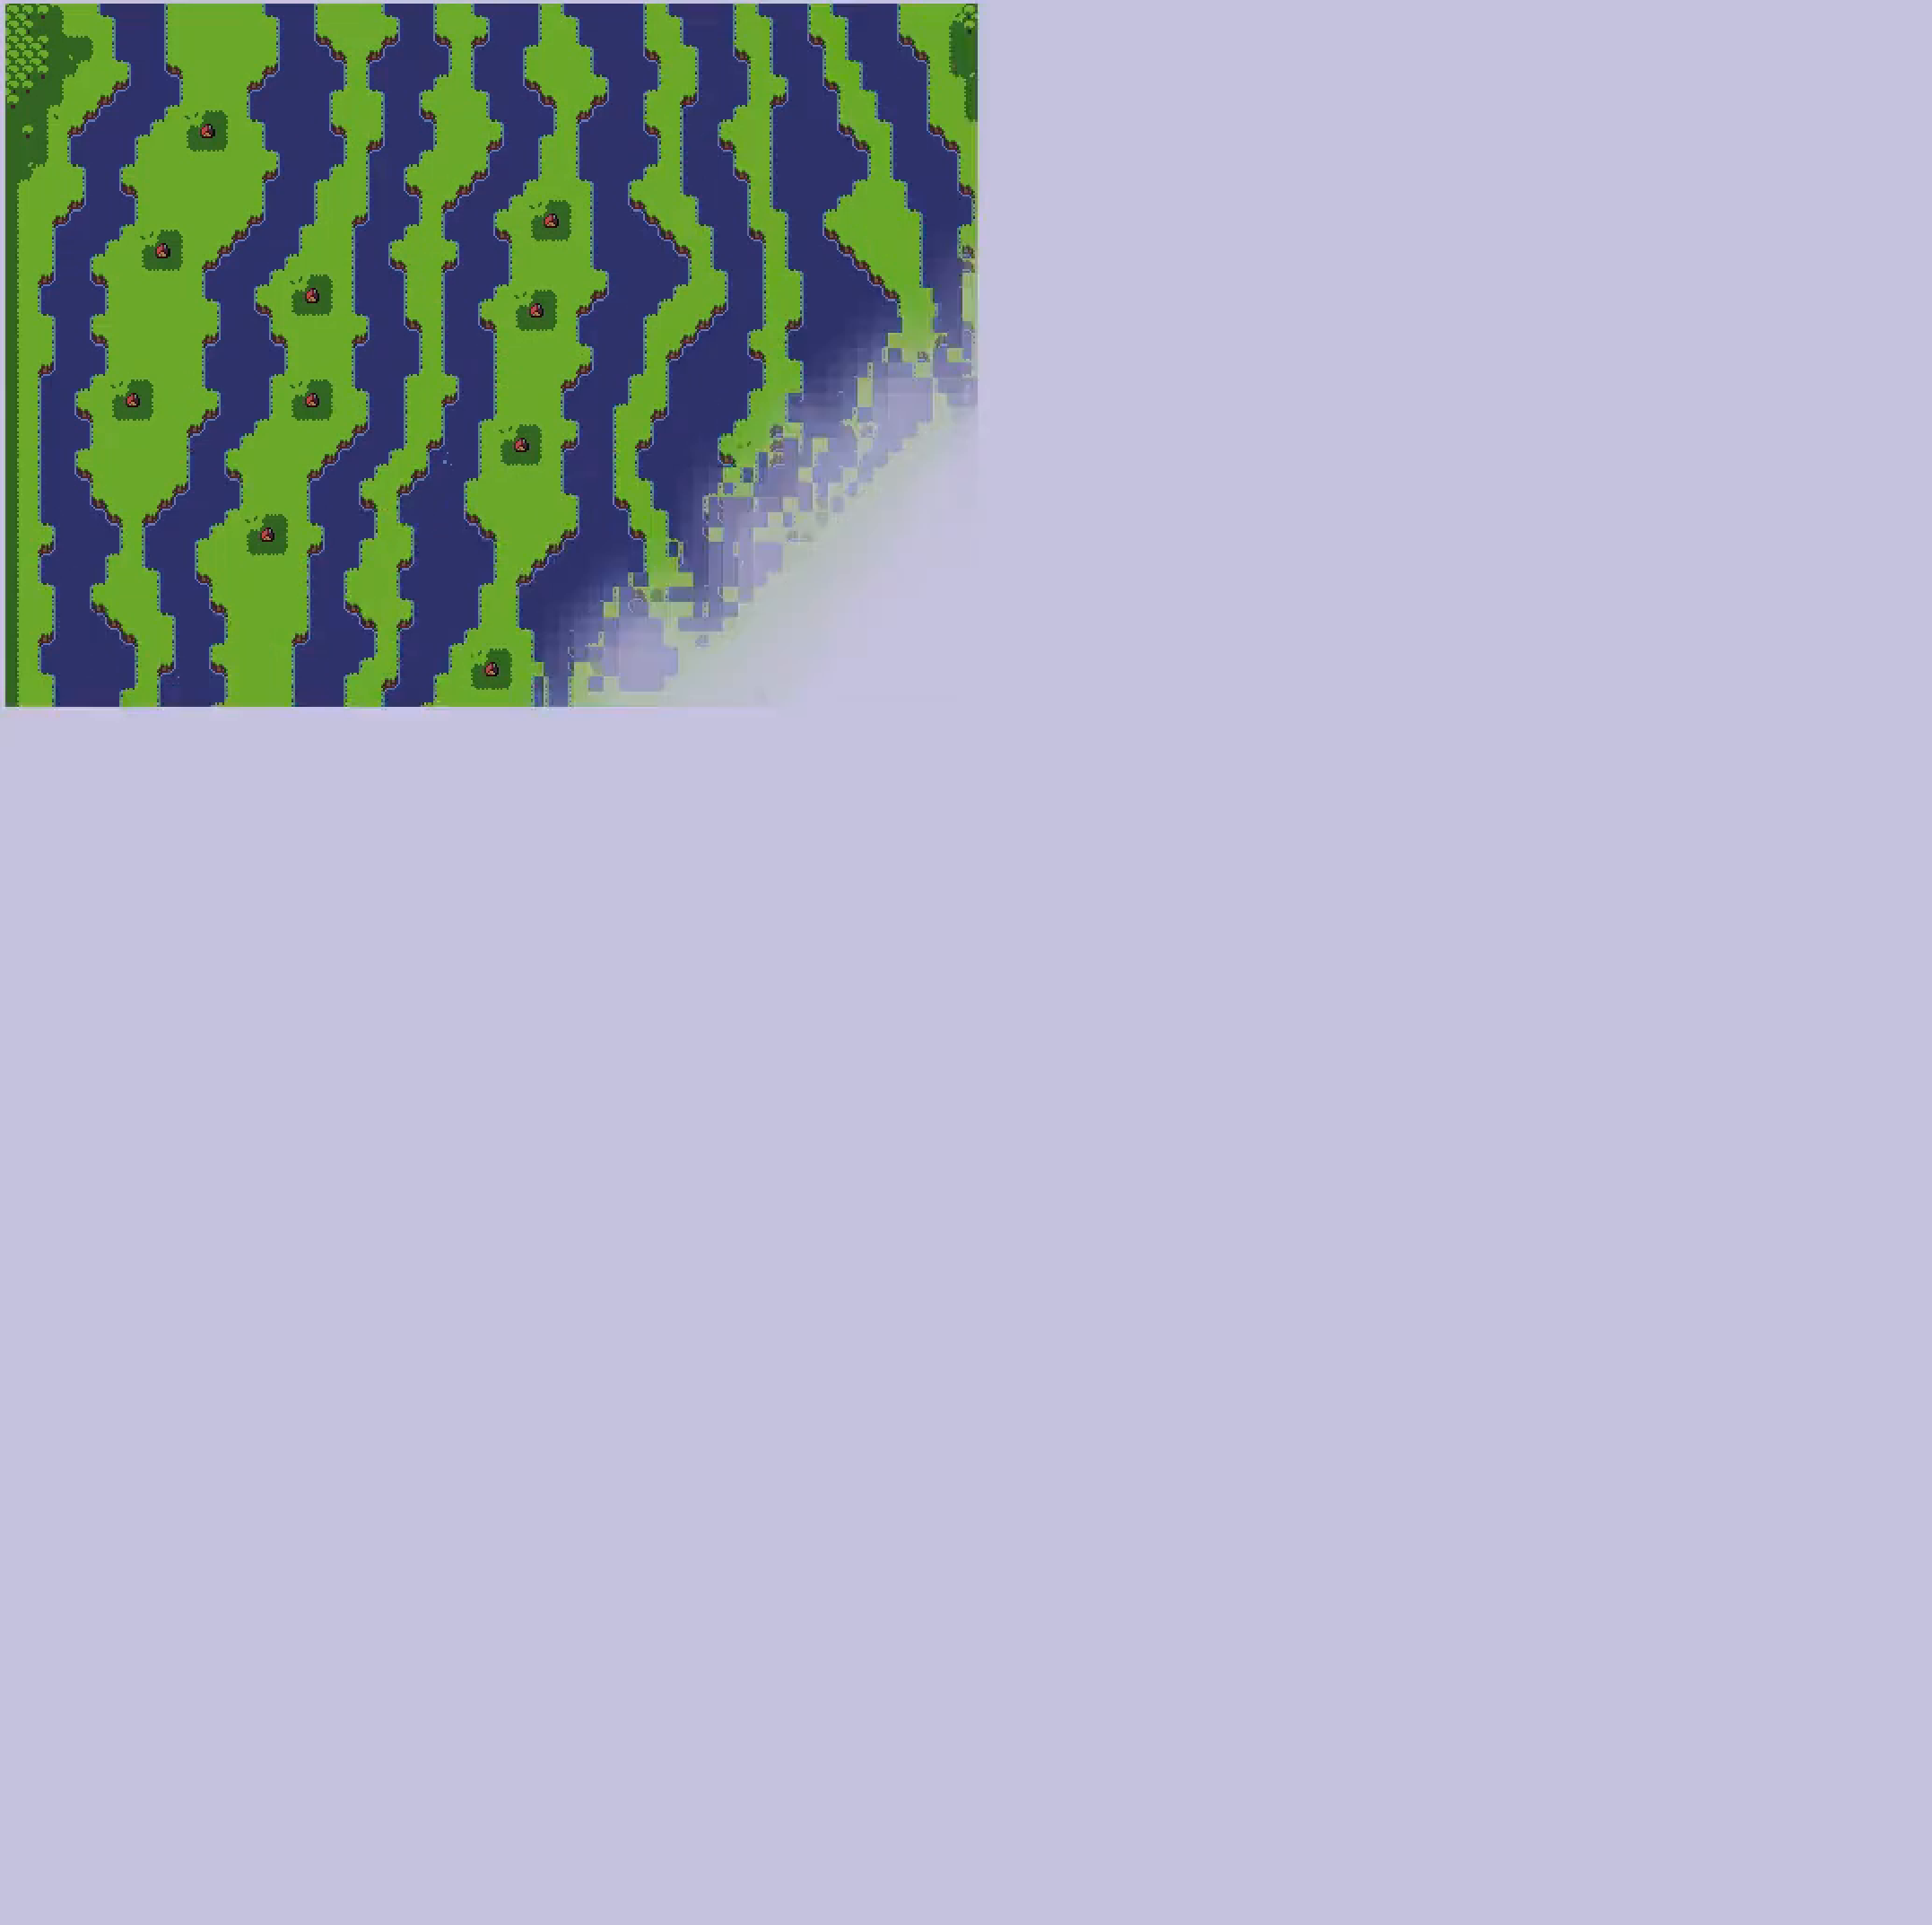
\includegraphics[width=\textwidth]{img/fm_0006.pdf}
%    \end{figure}
%  \end{frame}
%

  \section{Results}

  \begin{frame}[fragile]{Results}

    ...

  \end{frame}

  \section{Conclusion}

  \begin{frame}[fragile]{Conclusion}

    \begin{center}\url{https://github.com/zzyzek/PunchOutModelSynthesis}\end{center}

  \end{frame}


\end{document}
